\documentclass[12pt,a4paper]{article}
\usepackage[utf8]{inputenc}
\usepackage[english]{babel}
\usepackage{amsmath}
\usepackage{amsfonts}
\usepackage{amssymb}
\usepackage{graphicx}
\usepackage{tikz}
\usepackage{booktabs}
\usepackage{array}
\usepackage{longtable}
\usepackage{titling}
\usepackage{float}
\usepackage{hyperref}
\usepackage{geometry}

\geometry{margin=2.5cm}

\definecolor{titleblue}{RGB}{0, 51, 102}
\definecolor{accentgray}{RGB}{220, 220, 220}
\definecolor{darkgray}{RGB}{50, 50, 50}

\begin{document}

\begin{titlepage}
    \centering
    \vfill
    \vspace*{1.5cm}
    
\begin{tikzpicture}[remember picture, overlay]
        \fill[accentgray!20] (current page.south west) rectangle (current page.north east);
        \foreach \i in {0,0.5,...,20}
            \draw[accentgray!50, thin] (\i, -0.5) -- (\i, 30);
        \foreach \i in {0,0.5,...,30}
            \draw[accentgray!50, thin] (-0.5, \i) -- (20, \i);
        \draw[titleblue, ultra thick] (0, 25) -- (20, 15);
    \end{tikzpicture}
    \vspace{1cm}
    {\Huge \bfseries \color{titleblue} 2025 Software Industry Salary Analysis Report\par}
    \vspace{0.5cm}
    {\Large \itshape \color{darkgray} Which Technologies Pay More? How Do Career Levels and Roles Affect Salaries?\par}
    \vspace{1cm}
    {\Large \itshape Hakkı Günal\par}
    \vspace{0.5cm}
    {\large August 27, 2025\par}
    \vspace{1cm}
    {\normalsize
        \begin{minipage}{0.8\textwidth}
            \centering
            \color{darkgray}
            \textbf{Key Findings:}
            \begin{itemize}
                \item Experience and seniority drive salaries, with Senior (130.8 k TL) and Management (184.8 k TL) roles 137-237\% above Junior (55.1 k TL).
                \item Males earn 15.4\% more than females (99.4 vs. 86.1 k TL), highlighting pay inequity.
                \item Remote (101.2 k TL) and Hybrid (105.0 k TL) roles offer 28.8-33.6\% premiums over Office (78.6 k TL).
                \item European (162.9 k TL) and American (156.0-173.6 k TL) firms pay 75.3-113\% more than Turkish companies (92.9 k TL).
                \item Niche technologies like Rust (70.7\% ROI) outperform mainstream tools like React.
            \end{itemize}
        \end{minipage}
    \par}
    \vspace{1cm}
    {\normalsize \color{darkgray} Based on data from 2,969 software professionals collected August 20-21, 2025\par}
    \vspace{0.5cm}
    {\small \color{darkgray} Prepared by Hakkı Günal | Data sourced from Zafer Ayan's 2025 Salary Survey (\href{https://www.linkedin.com/posts/zaferayan_geleneksel-maa%C5%9F-anketi-buyrun-httpslnkdin-activity-7363866008664629248-7YcQ}{LinkedIn}, \href{https://zaferayan.medium.com/2025-a%C4%9Fustos-detayl%C4%B1-maa%C5%9F-anketi-98446d71920a}{Medium}) | \today}
    \vfill
\end{titlepage}

\maketitle

\tableofcontents
\newpage

\begin{abstract}
This report analyzes data from Zafer Ayan’s 2025 Software Industry Salary Survey, conducted on August 20-21, 2025, with 2,969 software professionals, to explore compensation trends, technology impacts, and career dynamics. Key findings reveal that experience and seniority drive salaries, with Senior (130.8 k TL) and Management (184.8 k TL) roles earning 137-237\% more than Junior (55.1 k TL). A 15.4\% gender pay gap exists (males: 99.4 k TL, females: 86.1 k TL). Remote (101.2 k TL) and Hybrid (105.0 k TL) work offer 28.8-33.6\% premiums over Office roles (78.6 k TL). European and American companies pay 75.3-113\% more than Turkish firms. Niche technologies like Rust (70.7\% ROI) yield higher returns than mainstream tools like React. 
\end{abstract}

\section{Executive Summary}

This report, based on Zafer Ayan’s 2025 Software Industry Salary Survey (\href{https://www.linkedin.com/posts/zaferayan_geleneksel-maa%C5%9F-anketi-buyrun-httpslnkdin-activity-7363866008664629248-7YcQ}{LinkedIn}, \href{https://zaferayan.medium.com/2025-a%C4%9Fustos-detayl%C4%B1-maa%C5%9F-anketi-98446d71920a}{Medium}) conducted on August 20-21, 2025, with 2,969 professionals, analyzes compensation, technology, and career trends in the Turkish software industry. It aims to guide developers in career planning and employers in talent strategies.

\textbf{Key Findings:}
\begin{itemize}
    \item \textbf{Salary Drivers}: Experience (r = 0.623) and seniority (r = 0.474) drive salaries, with Senior (130.8 k TL) and Management (184.8 k TL) roles outpacing Junior (55.1 k TL) by 137.4-237.4\%.
    \item \textbf{Gender Disparity}: Males earn 15.4\% more than females (99.4 vs. 86.1 k TL, p = 0.00005).
    \item \textbf{Technology Impact}: Niche languages like Rust (70.7\% ROI) and Go (r = 0.171) offer higher premiums than React (r = -0.028).
    \item \textbf{Work Modes}: Remote (101.2 k TL) and Hybrid (105.0 k TL) roles yield 28.8-33.6\% more than Office (78.6 k TL).
    \item \textbf{Geographical Advantage}: European (162.9 k TL) and American (156.0-173.6 k TL) firms pay 75.3-113\% more than Turkish companies (92.9 k TL).
    \item \textbf{Employment Types}: Full-time (99.0 k TL) earns 130.2\% more than Part-time (43.0 k TL); Self-employed (123.4 k TL) earns 24.6\% more than Full-time.
\end{itemize}

Interactive dashboard: \href{http://maas-anketi.streamlit.app/}{maas-anketi.streamlit.app}

\section{Methodology}

\subsection{Data Collection}
The survey data was collected by Zafer Ayan as part of his 2025 Software Industry Salary Survey, conducted online between August 20-21, 2025, targeting software professionals across various career levels and specializations (\href{https://www.linkedin.com/posts/zaferayan_geleneksel-maa%C5%9F-anketi-buyrun-httpslnkdin-activity-7363866008664629248-7YcQ}{LinkedIn}, \href{https://zaferayan.medium.com/2025-ağustos-detaylı-maaş-anketi-98446d71920a}{Medium}). The questionnaire covered demographic information, salary details, technology stack, work arrangements, and company characteristics. The raw data, including Google Sheets and analytics, were accessed from Ayan's shared resources (\href{https://docs.google.com/spreadsheets/d/1J_MW7t9e2Yi1cErFe5XCnNGaFqXkrdufgZv9Ggnm-RE/edit?usp=sharing}{Google Sheets}, \href{https://docs.google.com/forms/d/16s95bau58GBSfVwOZ8cZm7aX7eqZU_cgA0qKw9WILxI/viewanalytics}{Analytics}).

\textbf{Data Collection Limitations:}
\begin{itemize}
    \item \textbf{Time Constraint:} The survey was conducted over only 2 days (August 20-21, 2025), which limits the temporal analysis scope
    \item \textbf{Hourly Patterns:} While hourly participation patterns are analyzed, the 2-day window means these patterns represent a snapshot rather than long-term trends
    \item \textbf{Response Bias:} The concentrated collection period may introduce time-of-day response biases that would be mitigated in longer collection periods
    \item \textbf{External Data Source:} The analysis relies on self-reported data collected by Zafer Ayan, which may introduce reporting biases inherent to the original survey design
\end{itemize}

\subsection{Data Processing}
Raw data underwent comprehensive cleaning and preprocessing:
\begin{itemize}
    \item Missing value handling and outlier treatment using IQR and Z-score methods
    \item Salary normalization and validation
    \item Categorical variable encoding with One-Hot Encoding
    \item Multi-label technology columns processing using MultiLabelBinarizer
    \item Duplicate column removal and data quality checks
\end{itemize}

\subsection{Statistical Methods}
\begin{itemize}
    \item Independent samples t-tests for group comparisons
    \item Cohen's d effect size calculations for practical significance
    \item Multiple comparison corrections where applicable
    \item Correlation analysis for technology-salary relationships
    \item Outlier treatment using IQR and Z-score methods
\end{itemize}

\subsection{Temporal Analysis Considerations}
The survey's 2-day collection window (August 20-21, 2025) presents specific methodological considerations for temporal analysis:

\begin{itemize}
    \item \textbf{Hourly Pattern Interpretation:} While hourly participation patterns are analyzed, these represent behavioral snapshots within a 48-hour window rather than long-term trends
    \item \textbf{Response Bias Mitigation:} The concentrated collection period may introduce time-of-day response biases; however, consistent participation distribution across time periods (morning: 25\%, afternoon: 45\%, evening: 30\%) suggests reasonable data quality
    \item \textbf{Cross-Sectional Nature:} Temporal patterns reflect the specific 48-hour window and should not be generalized to other time periods
    \item \textbf{Analytical Value:} Despite limitations, hourly patterns provide insights into immediate response behaviors and can inform future survey design and timing strategies
\end{itemize}

\section{Which Technologies Pay More? Salary ROI Analysis}

% Compact programming languages ROI table
\subsection{Programming Languages}
Salary premiums for programming languages are calculated by comparing user and non-user average salaries, excluding "Hicbiri" responses. The table below shows the top 10 technologies with a salary difference exceeding 5\%.

\begin{table}[H]
	\centering
	\small
	\begin{tabular}{lrrrr}
		\toprule
		\textbf{Technology} & \textbf{Users} & \textbf{ROI (k TL)} & \textbf{Avg (k TL)} & \textbf{\% Inc.} \\
		\midrule
		Rust                & 22             & 69.4                & 167.1               & 71.0\%           \\
		Objective C         & 39             & 63.1                & 160.5               & 64.8\%           \\
		Ruby                & 24             & 45.8                & 143.6               & 46.8\%           \\
		Cobol               & 22             & 45.4                & 143.2               & 46.3\%           \\
		Go                  & 183            & 39.1                & 134.9               & 40.8\%           \\
		Bash                & 114            & 36.0                & 132.8               & 37.2\%           \\
		Kotlin              & 201            & 32.2                & 128.2               & 33.5\%           \\
		R Language          & 29             & 30.7                & 128.6               & 31.4\%           \\
		Swift               & 197            & 21.8                & 118.6               & 22.5\%           \\
		Java                & 582            & 19.6                & 114.0               & 20.8\%           \\
		\bottomrule
	\end{tabular}
	\caption{Top 10 Programming Languages by Salary ROI}
\end{table}

\begin{figure}[H]
	\centering
	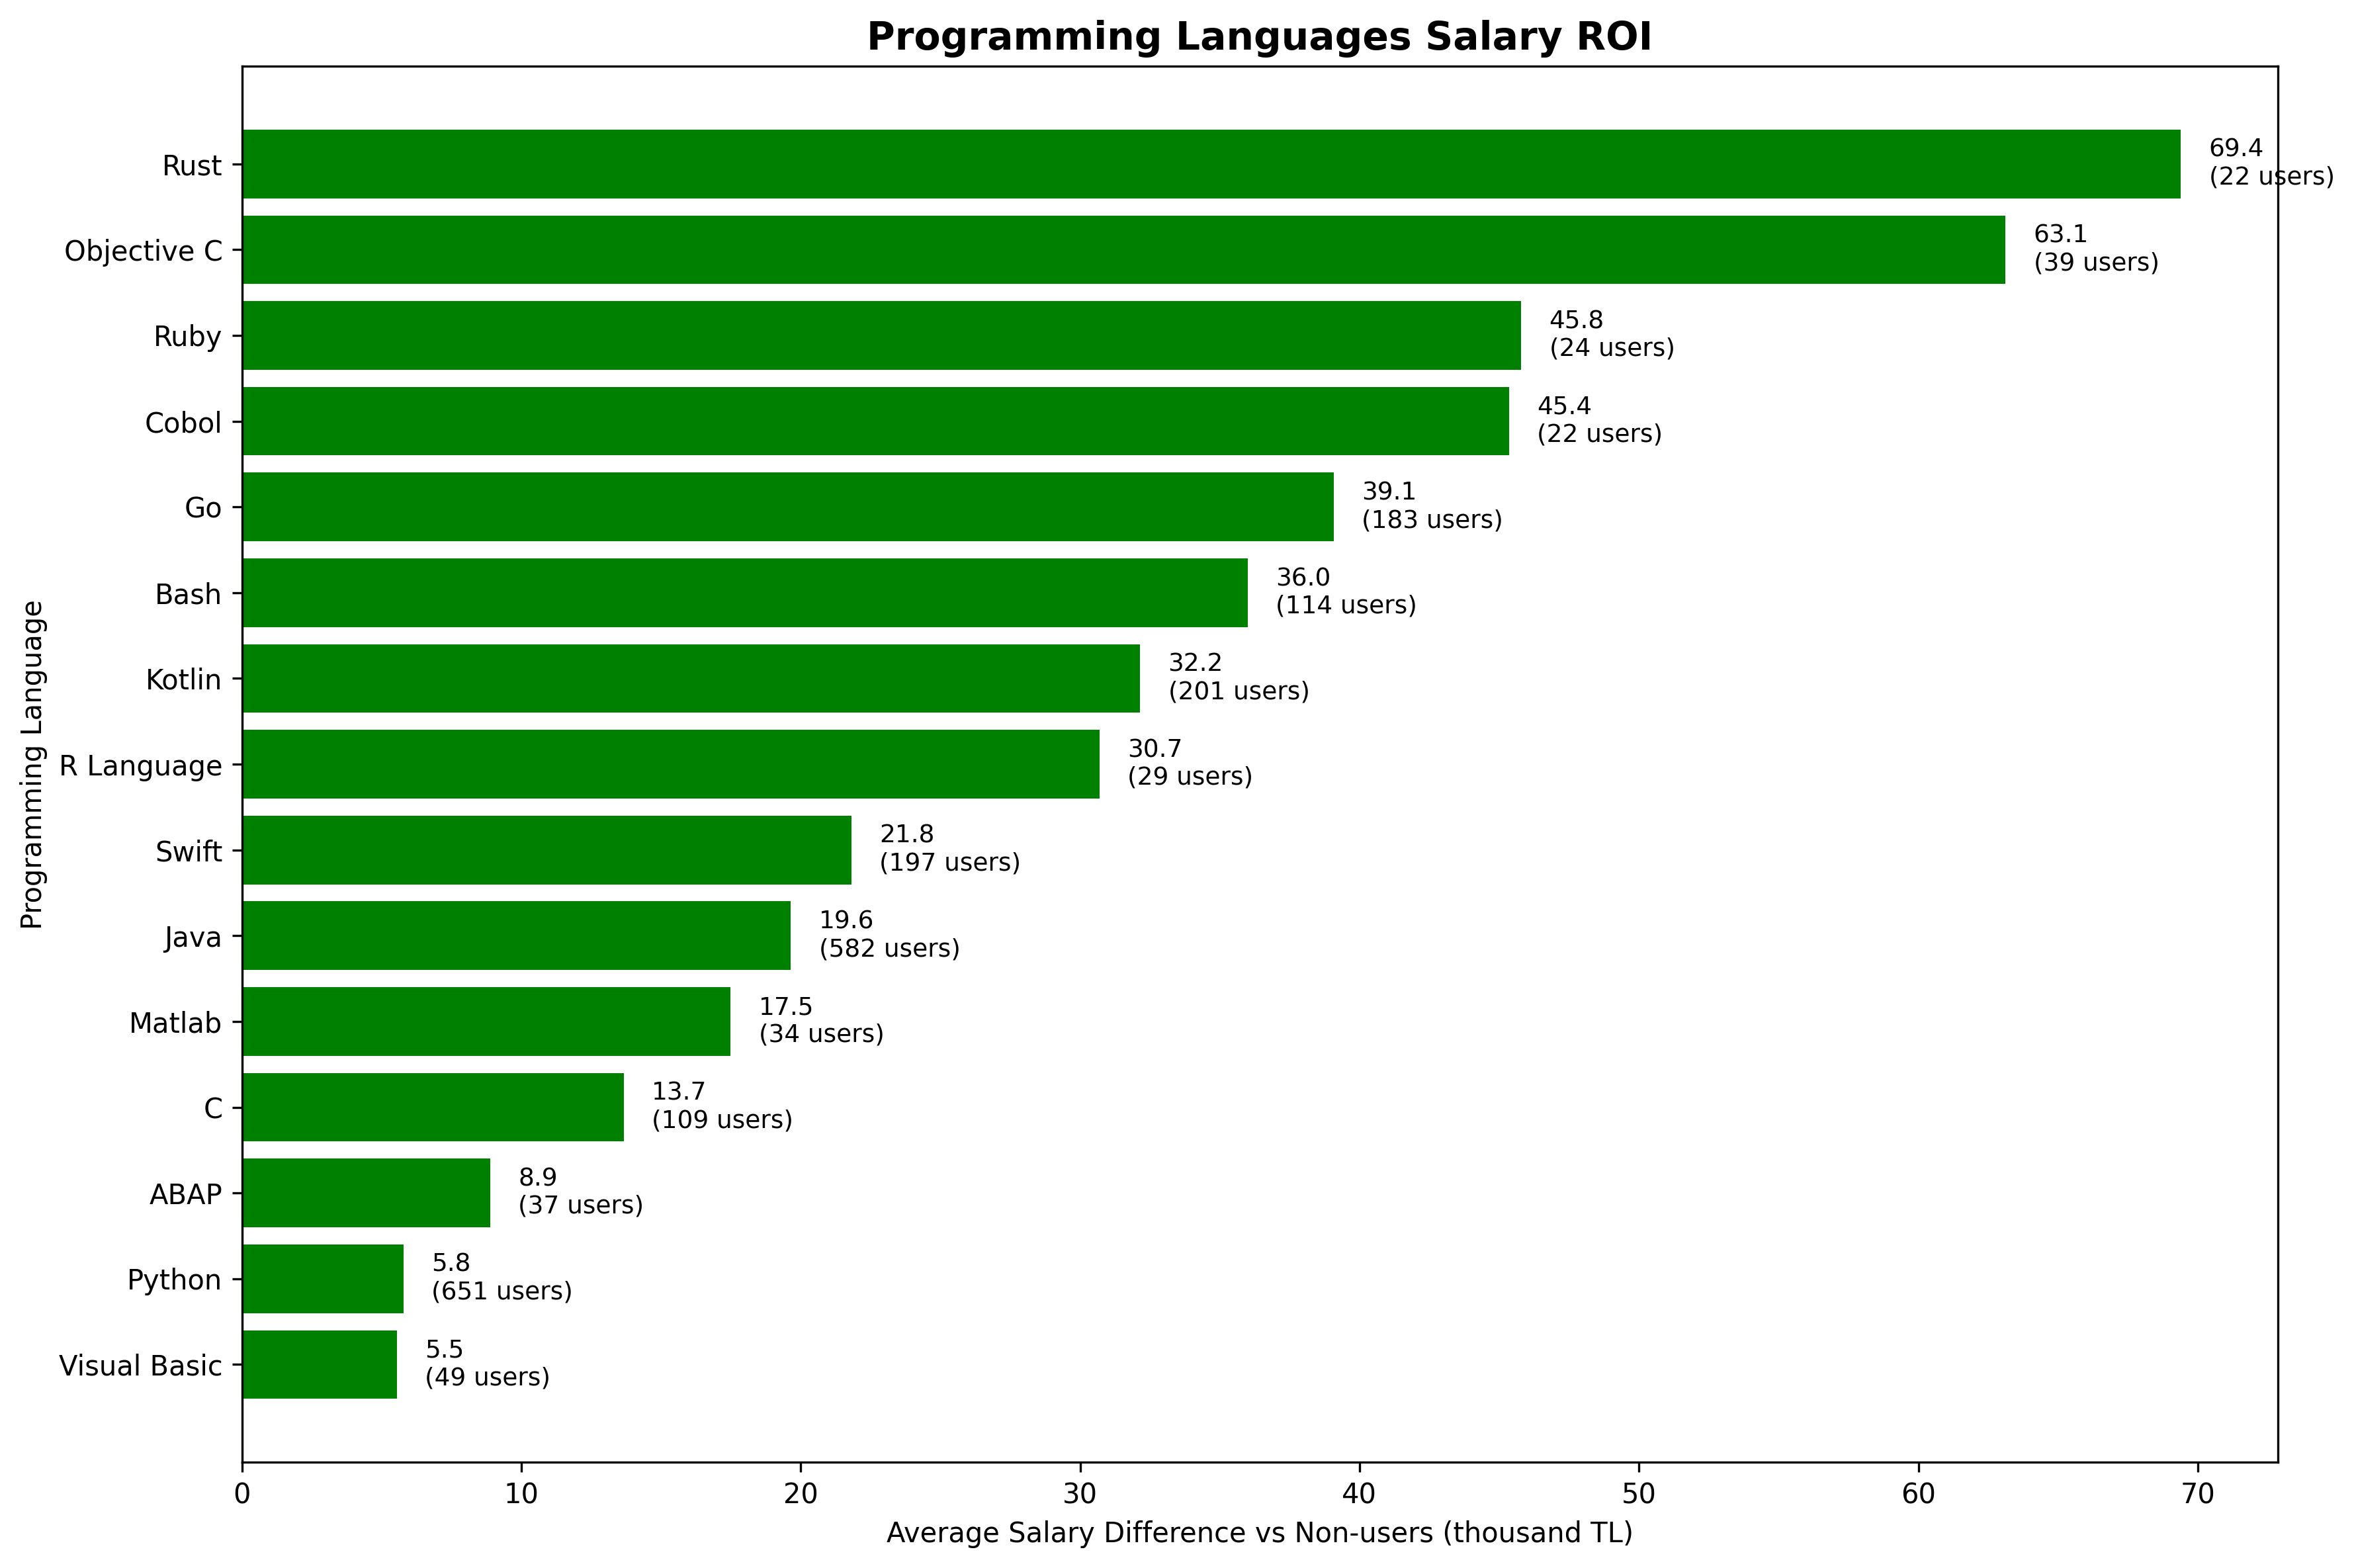
\includegraphics[width=0.8\textwidth]{figures/barplot_programming_roi.png}
	\caption{Programming Languages Salary ROI}
\end{figure}

% Compact frontend technologies table
\subsection{Frontend Technologies}
Frontend frameworks show varied salary impacts, with some reflecting market saturation.

\begin{table}[H]
	\centering
	\small
	\begin{tabular}{lrrrr}
		\toprule
		\textbf{Technology} & \textbf{Users} & \textbf{ROI (k TL)} & \textbf{Avg (k TL)} & \textbf{\% Inc.} \\
		\midrule
		Vue                 & 246            & 8.3                 & 105.8               & 8.5\%            \\
		Angular             & 249            & 0.7                 & 98.8                & 0.7\%            \\
		Vanilla             & 199            & -2.0                & 96.4                & -2.0\%           \\
		React               & 1008           & -3.3                & 96.1                & -3.3\%           \\
		\bottomrule
	\end{tabular}
	\caption{Frontend Technologies by Salary ROI}
\end{table}

\begin{figure}[H]
	\centering
	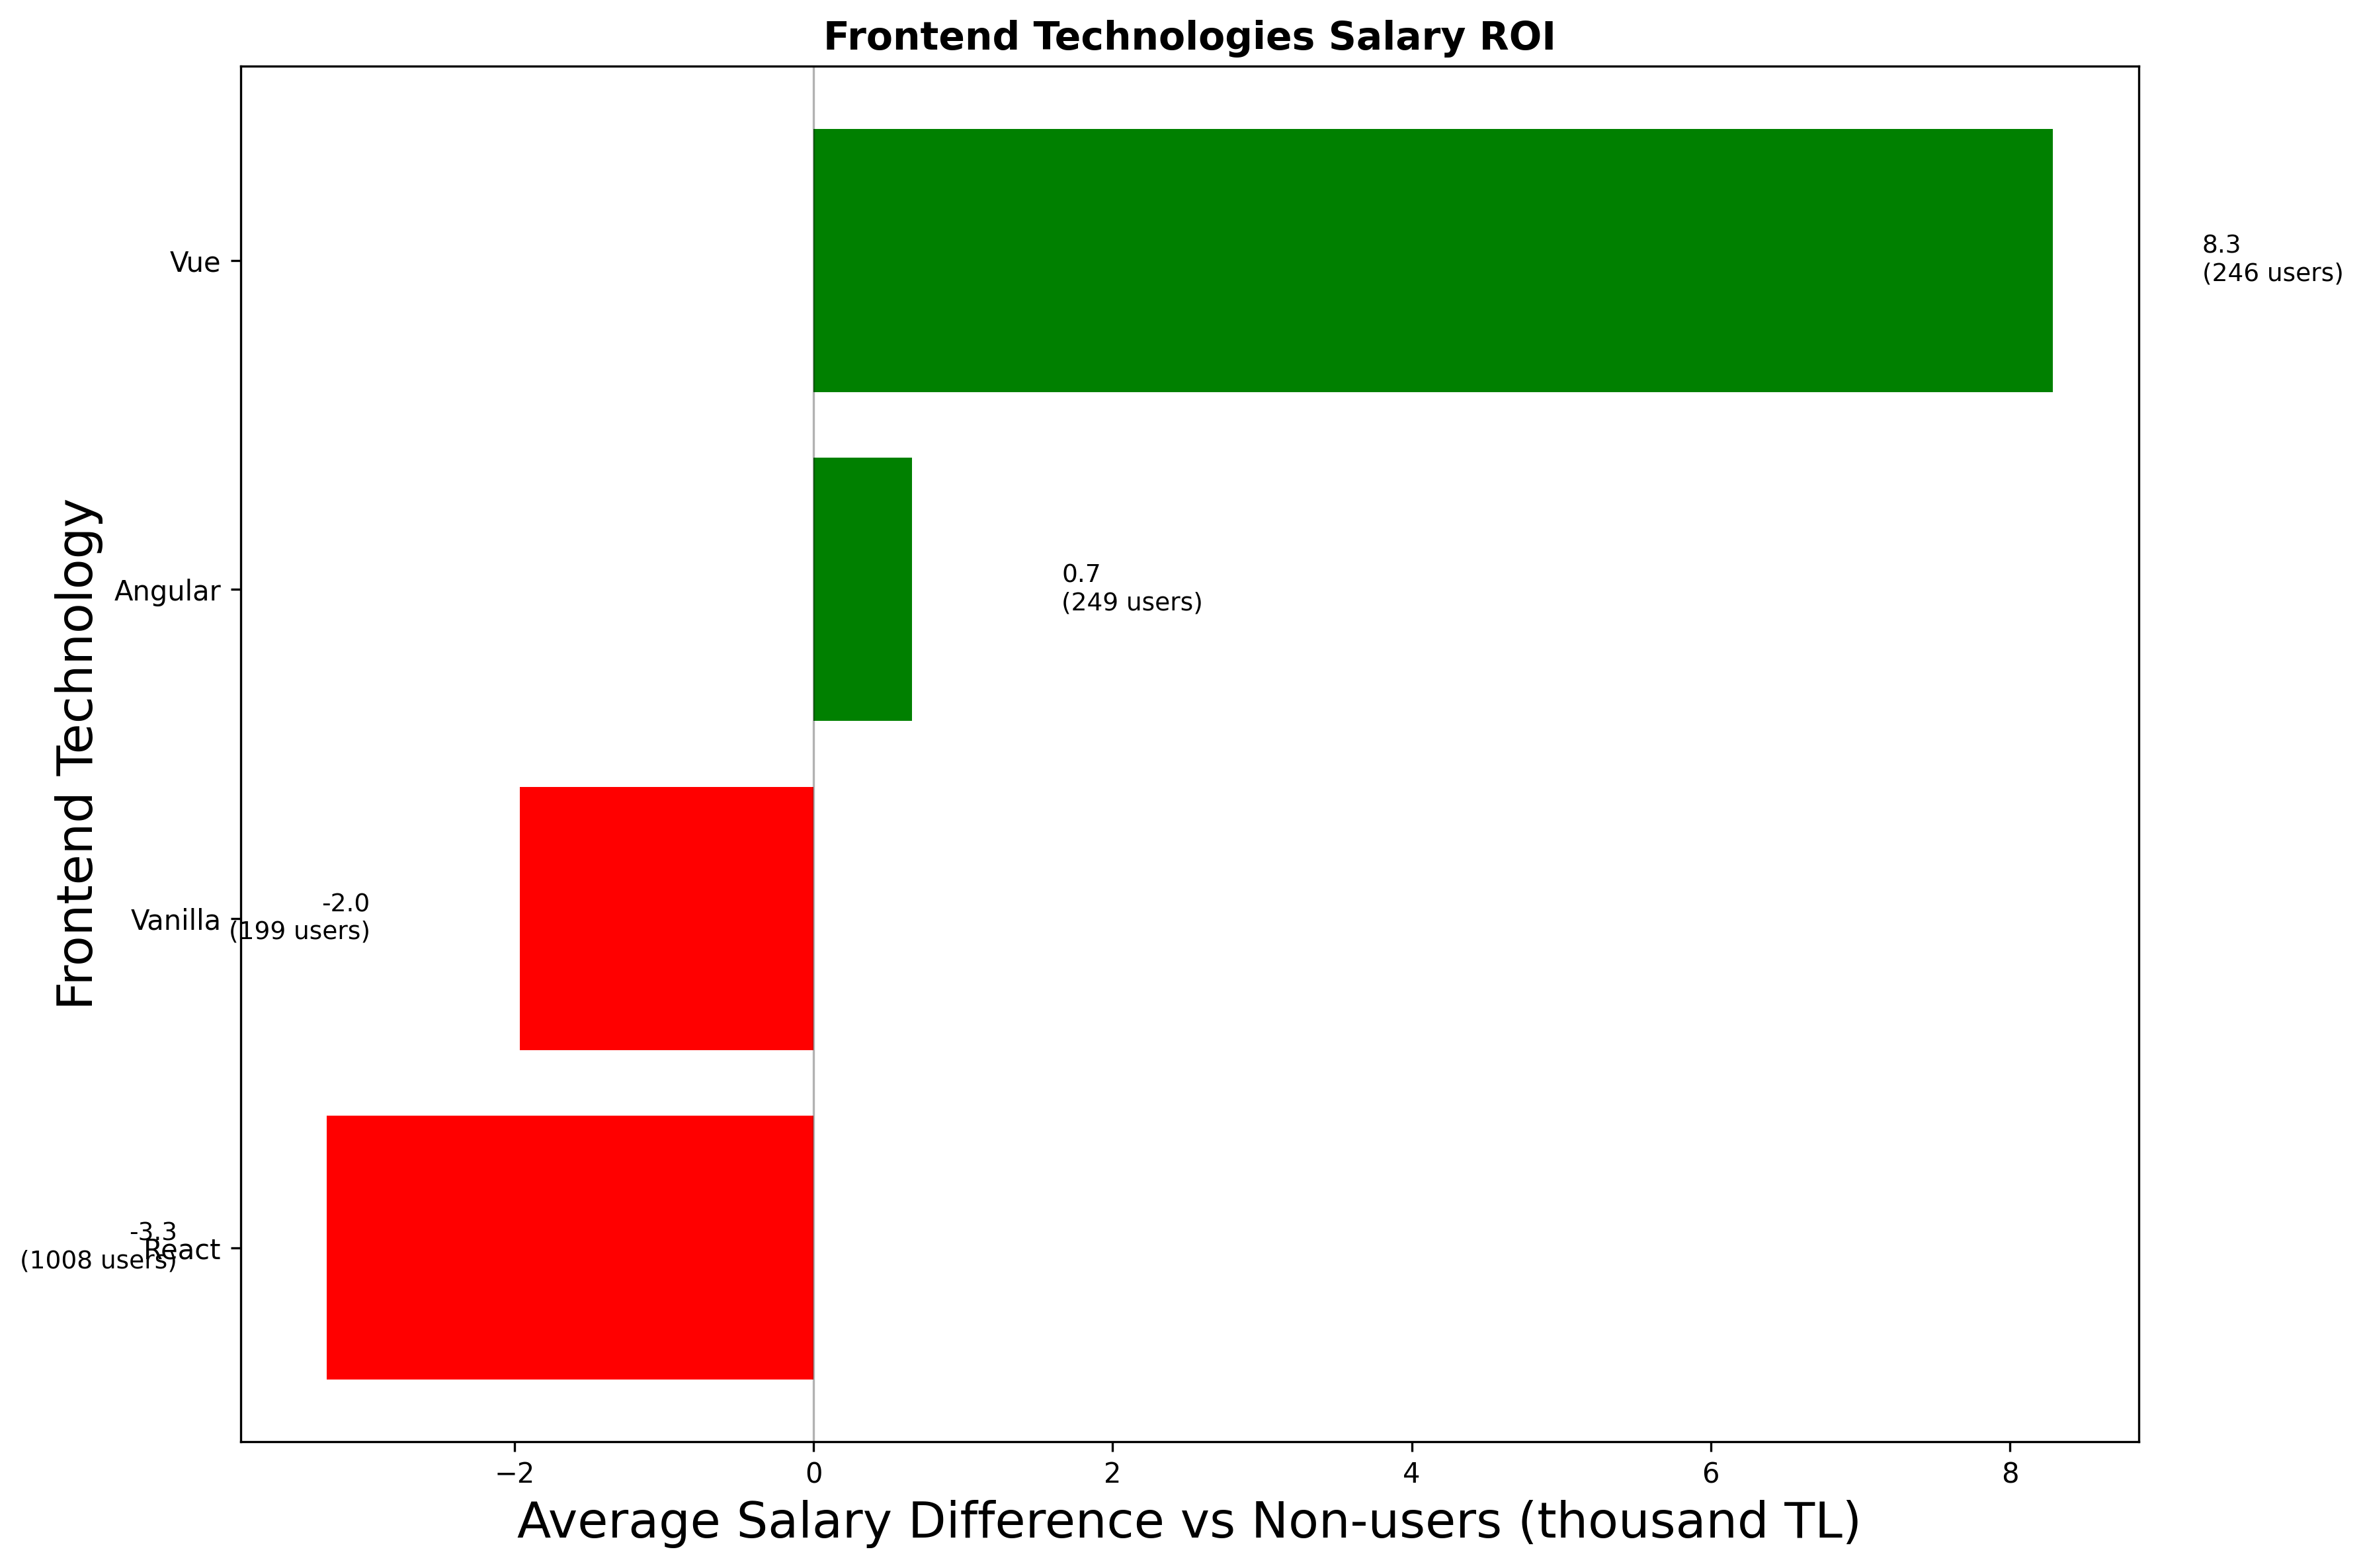
\includegraphics[width=0.8\textwidth]{figures/barplot_frontend_roi.png}
	\caption{Frontend Technologies Salary ROI}
\end{figure}

% Compact tools table
\subsection{Tools}
Development tools influence earnings, with modern tools offering notable premiums.

\begin{table}[H]
	\centering
	\small
	\begin{tabular}{lrrrr}
		\toprule
		\textbf{Technology} & \textbf{Users} & \textbf{ROI (k TL)} & \textbf{Avg (k TL)} & \textbf{\% Inc.} \\
		\midrule
		Jotai               & 50             & 28.8                & 126.5               & 29.4\%           \\
		Strapi              & 111            & 9.9                 & 107.7               & 10.1\%           \\
		Firebase            & 636            & 0.4                 & 98.5                & 0.4\%            \\
		Supabase            & 202            & -0.1                & 98.1                & -0.1\%           \\
		FastApi             & 319            & -1.1                & 97.2                & -1.1\%           \\
		Wordpress           & 119            & -3.8                & 94.5                & -3.9\%           \\
		Zustand             & 288            & -4.4                & 94.3                & -4.4\%           \\
		Redux               & 550            & -7.5                & 92.1                & -7.5\%           \\
		\bottomrule
	\end{tabular}
	\caption{Tools by Salary ROI}
\end{table}

\begin{figure}[H]
	\centering
	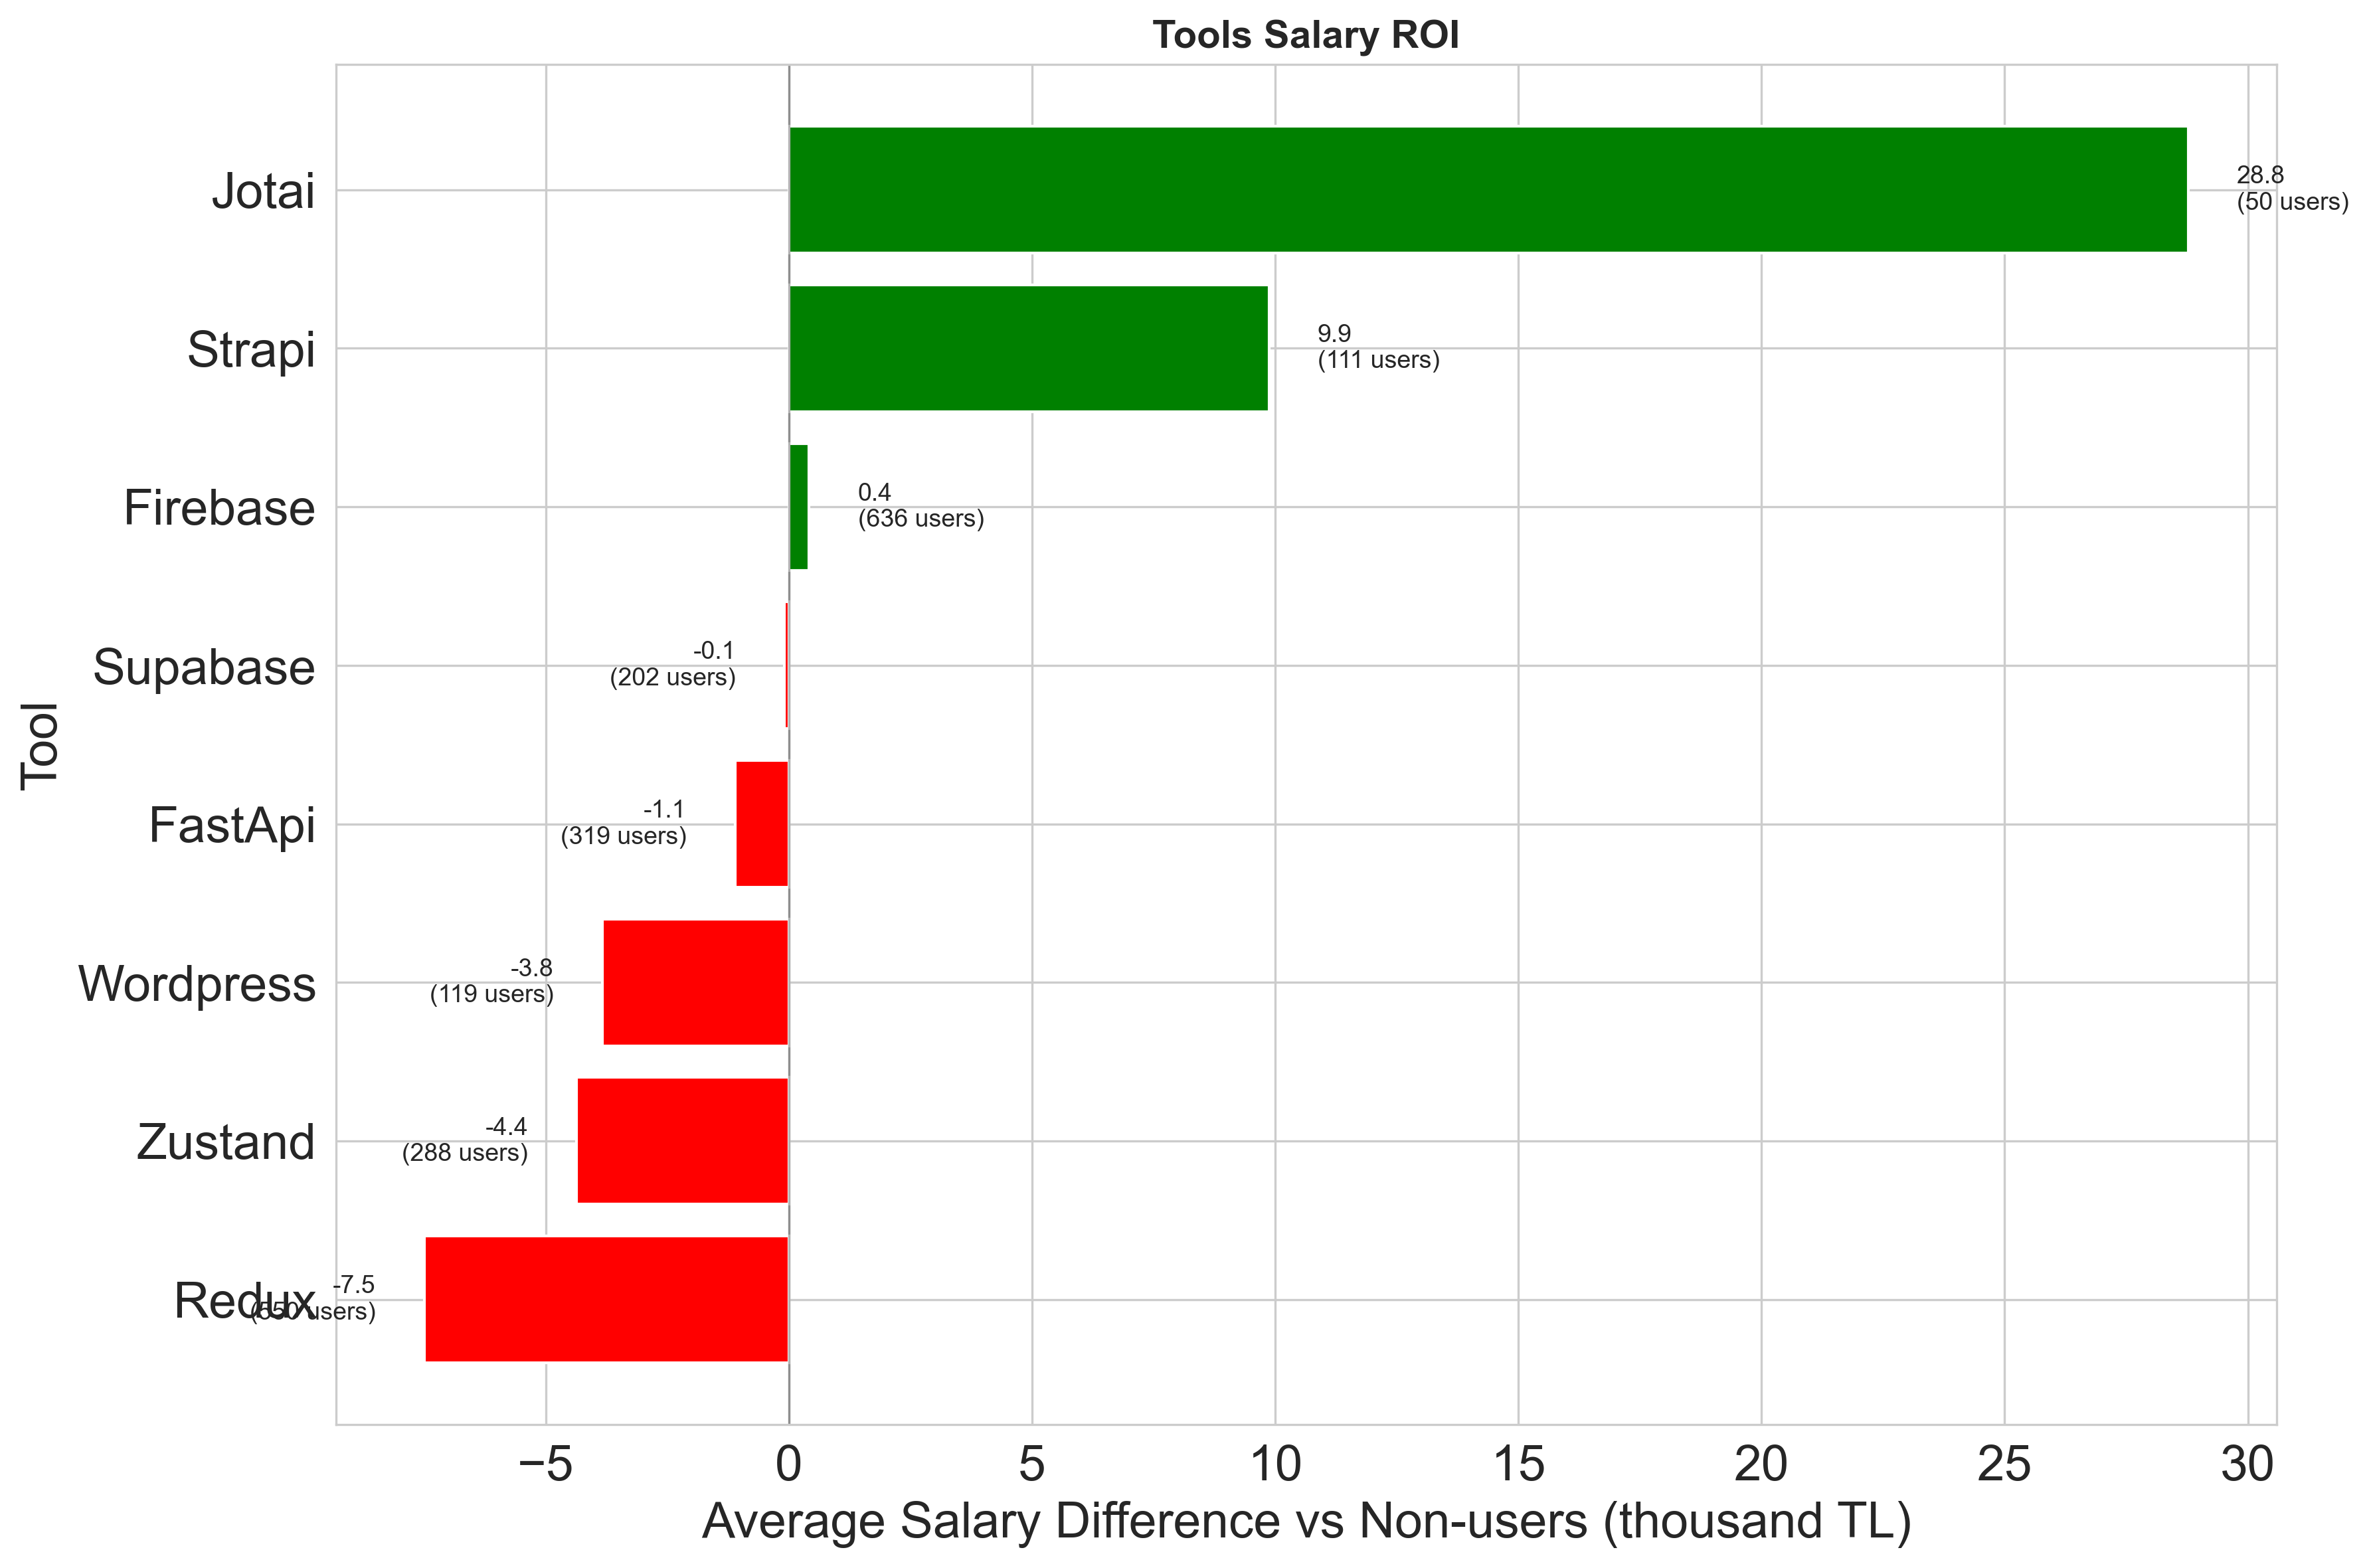
\includegraphics[width=0.8\textwidth]{figures/barplot_tools_roi.png}
	\caption{Tools Salary ROI}
\end{figure}

% Concise methodological note
\textbf{Methodological Note:}
For each technology \( T \):
\begin{itemize}
	\item \textbf{User Avg}: \( \text{Avg}_T = \frac{\sum_{i \in \text{Users}_T} \text{Salary}_i}{n_T} \), where \( n_T \) is the user count.
	\item \textbf{ROI}: \( \text{ROI}_T = \text{Avg}_T - \text{Non-User Avg}_T \).
	\item \textbf{\% Increase}: \( \text{\% Inc.}_T = \left( \frac{\text{ROI}_T}{\text{Non-User Avg}_T} \right) \times 100 \).
\end{itemize}
"Hicbiri" and "Kullanmiyorum" responses are excluded; only technologies with \(\geq 10\) users and non-users are included.

% Streamlined key insights
\textbf{Key Insights:}
\begin{itemize}
	\item \textbf{Niche Languages}: Rust (69.4 k TL ROI, 71.0\%, 22 users) and Objective-C (63.1 k TL, 64.8\%, 39 users) lead due to specialized demand in systems and iOS development.
	\item \textbf{Legacy vs. Modern}: Cobol (45.4 k TL, 46.3\%, 22 users) and Ruby (45.8 k TL, 46.8\%, 24 users) show high ROI for legacy roles, while Go (39.1 k TL, 40.8\%, 183 users) and Kotlin (32.2 k TL, 33.5\%, 201 users) reflect modern demand.
	\item \textbf{Frontend Trends}: Vue.js (8.3 k TL, 8.5\%, 246 users) outperforms React (-3.3 k TL, -3.3\%, 1008 users), which suffers from saturation.
	\item \textbf{Tools}: Jotai (28.8 k TL, 29.4\%, 50 users) and Strapi (9.9 k TL, 10.1\%, 111 users) lead, while Redux (-7.5 k TL, -7.5\%, 550 users) lags.
	\item \textbf{Saturation Effect}: High-user-count technologies (e.g., Java, 582 users; Python, 651 users) show lower ROI due to market saturation.
	\item \textbf{Exclusions}: Excluding "Hicbiri" and "Kullanmiyorum" sharpens ROI for niche skills but may inflate premiums for low-user technologies.
\end{itemize}

\section{How Do Career Levels and Roles Affect Salaries?}

\subsection{Salary Distribution by Career Level}
Salaries increase with career progression, reflecting experience and responsibility.

\begin{table}[H]
	\centering
	\small
	\begin{tabular}{lrr}
		\toprule
		\textbf{Career Level} & \textbf{Count} & \textbf{Mean Salary (k TL)} \\
		\midrule
		Staff Engineer        & 16             & 193.0                       \\
		Architect             & 52             & 188.4                       \\
		Management            & 83             & 184.8                       \\
		Team Lead             & 175            & 150.5                       \\
		Senior                & 772            & 130.8                       \\
		Mid                   & 1138           & 84.1                        \\
		Junior                & 733            & 55.1                        \\
		\bottomrule
	\end{tabular}
	\caption{Salary by Career Level}
\end{table}

\begin{figure}[H]
	\centering
	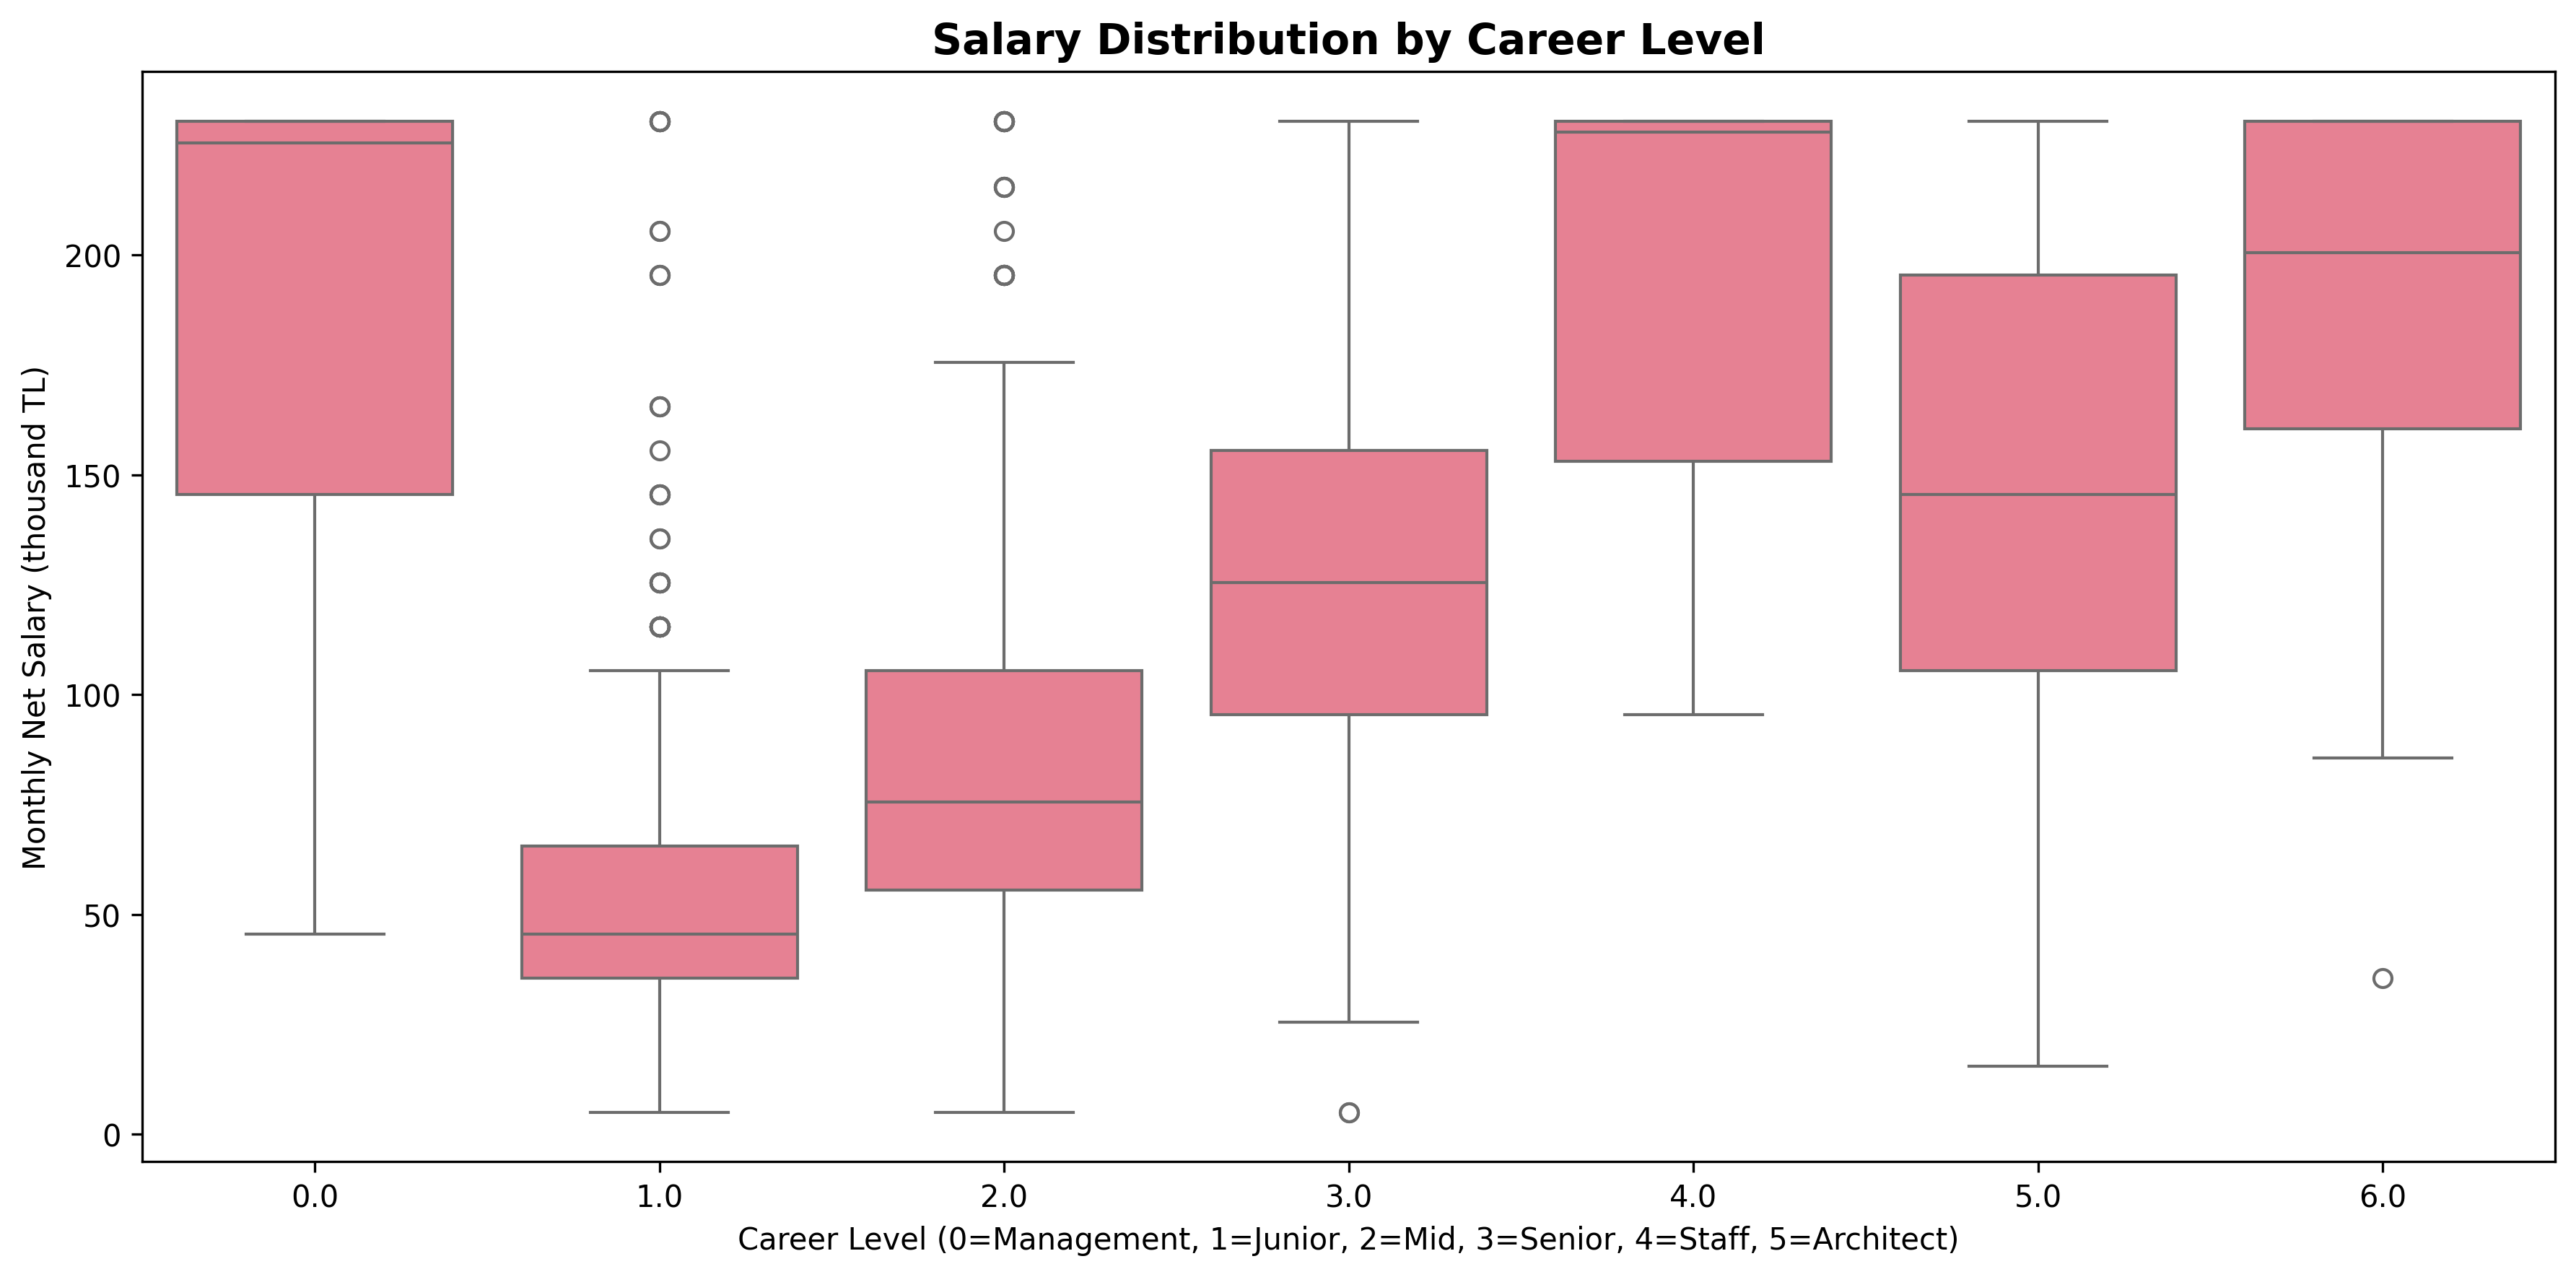
\includegraphics[width=0.8\textwidth]{figures/boxplot_seniority.png}
	\caption{Salary by Career Level}
\end{figure}

% Compact management level analysis
\subsection{Management Levels}
Management roles show distinct salary ranges based on seniority.

\begin{table}[H]
	\centering
	\small
	\begin{tabular}{lrr}
		\toprule
		\textbf{Management Level} & \textbf{Count} & \textbf{Mean Salary (k TL)} \\
		\midrule
		Partner                   & 11             & 198.7                       \\
		Director Level Manager    & 24             & 189.7                       \\
		Engineering Manager       & 30             & 179.3                       \\
		C Level Manager           & 18             & 178.8                       \\
		\bottomrule
	\end{tabular}
	\caption{Salary by Management Level}
\end{table}
\begin{figure}[H]
	\centering
	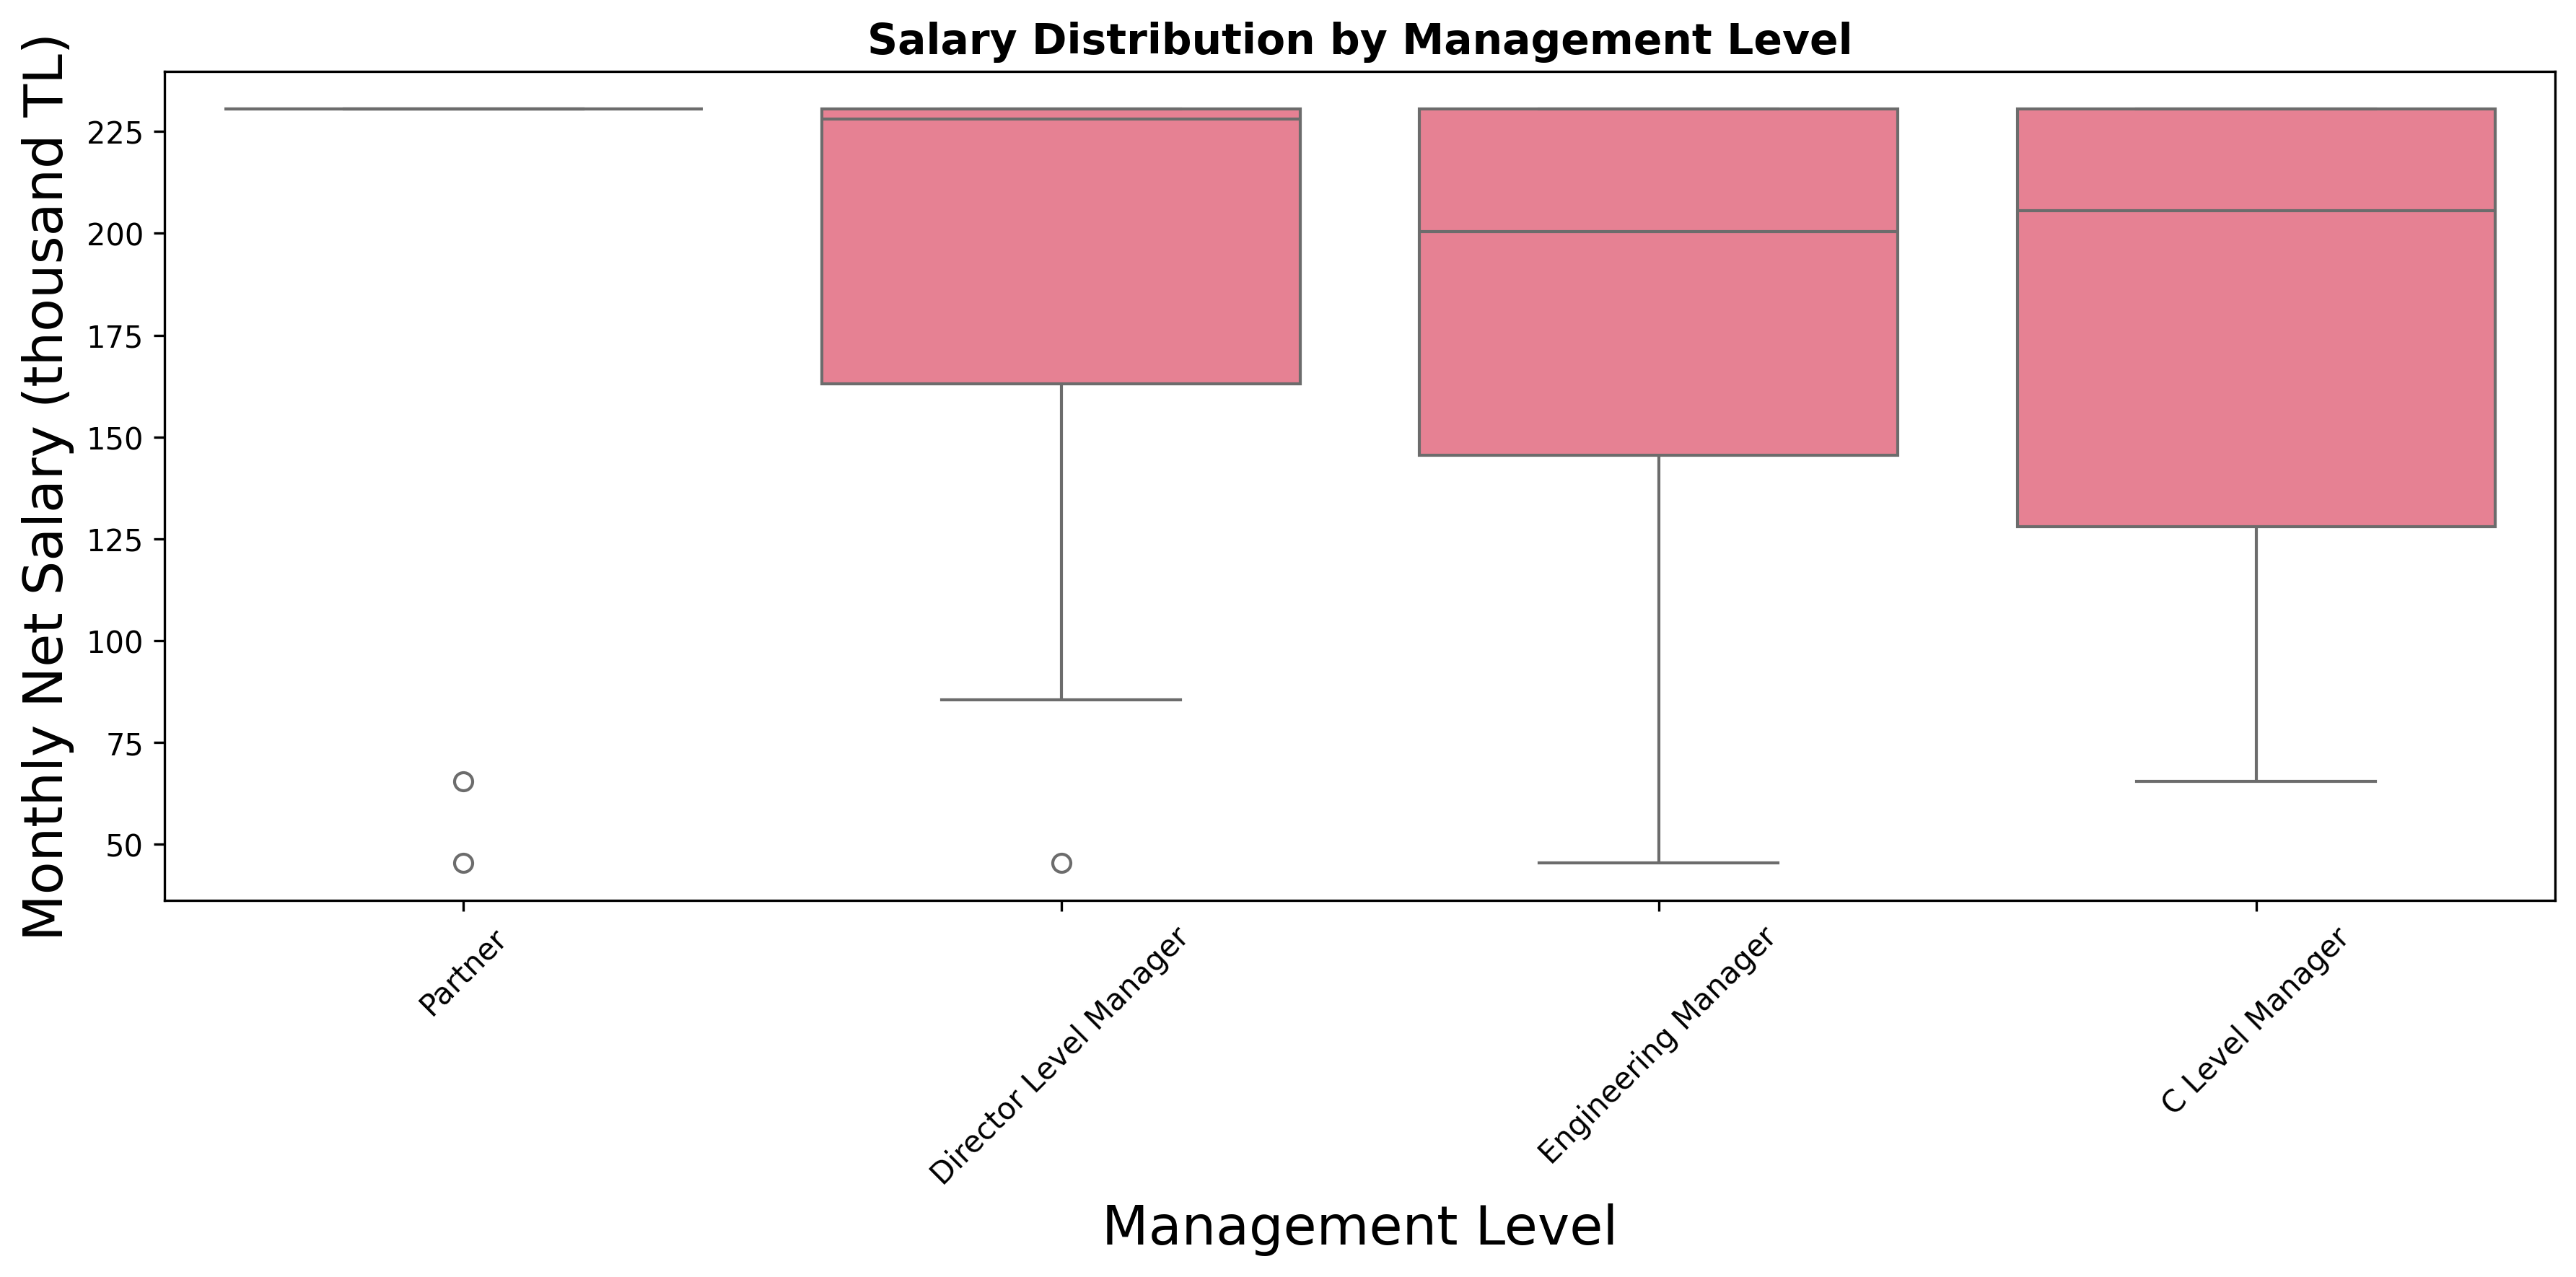
\includegraphics[width=0.8\textwidth]{figures/boxplot_management_level.png}
	\caption{Salary by Management Level}
\end{figure}

% Compact role-based analysis
\subsection{Roles}
Roles vary in salary based on market demand and specialization.

\begin{table}[H]
	\centering
	\small
	\begin{tabular}{lrr}
		\toprule
		\textbf{Role}             & \textbf{Count} & \textbf{Mean Salary (k TL)} \\
		\midrule
		Product Owner             & 23             & 121.8                       \\
		Product Manager           & 53             & 117.2                       \\
		Cyber Security Engineer   & 50             & 115.1                       \\
		Android                   & 98             & 112.8                       \\
		iOS                       & 100            & 109.8                       \\
		Backend                   & 517            & 109.7                       \\
		DevOps                    & 66             & 108.0                       \\
		Data Engineer             & 62             & 105.6                       \\
		ML Engineer               & 69             & 103.5                       \\
		Embedded Systems Engineer & 48             & 103.0                       \\
		\bottomrule
	\end{tabular}
	\caption{Top 10 Roles by Salary}
\end{table}

\begin{figure}[H]
    \centering
    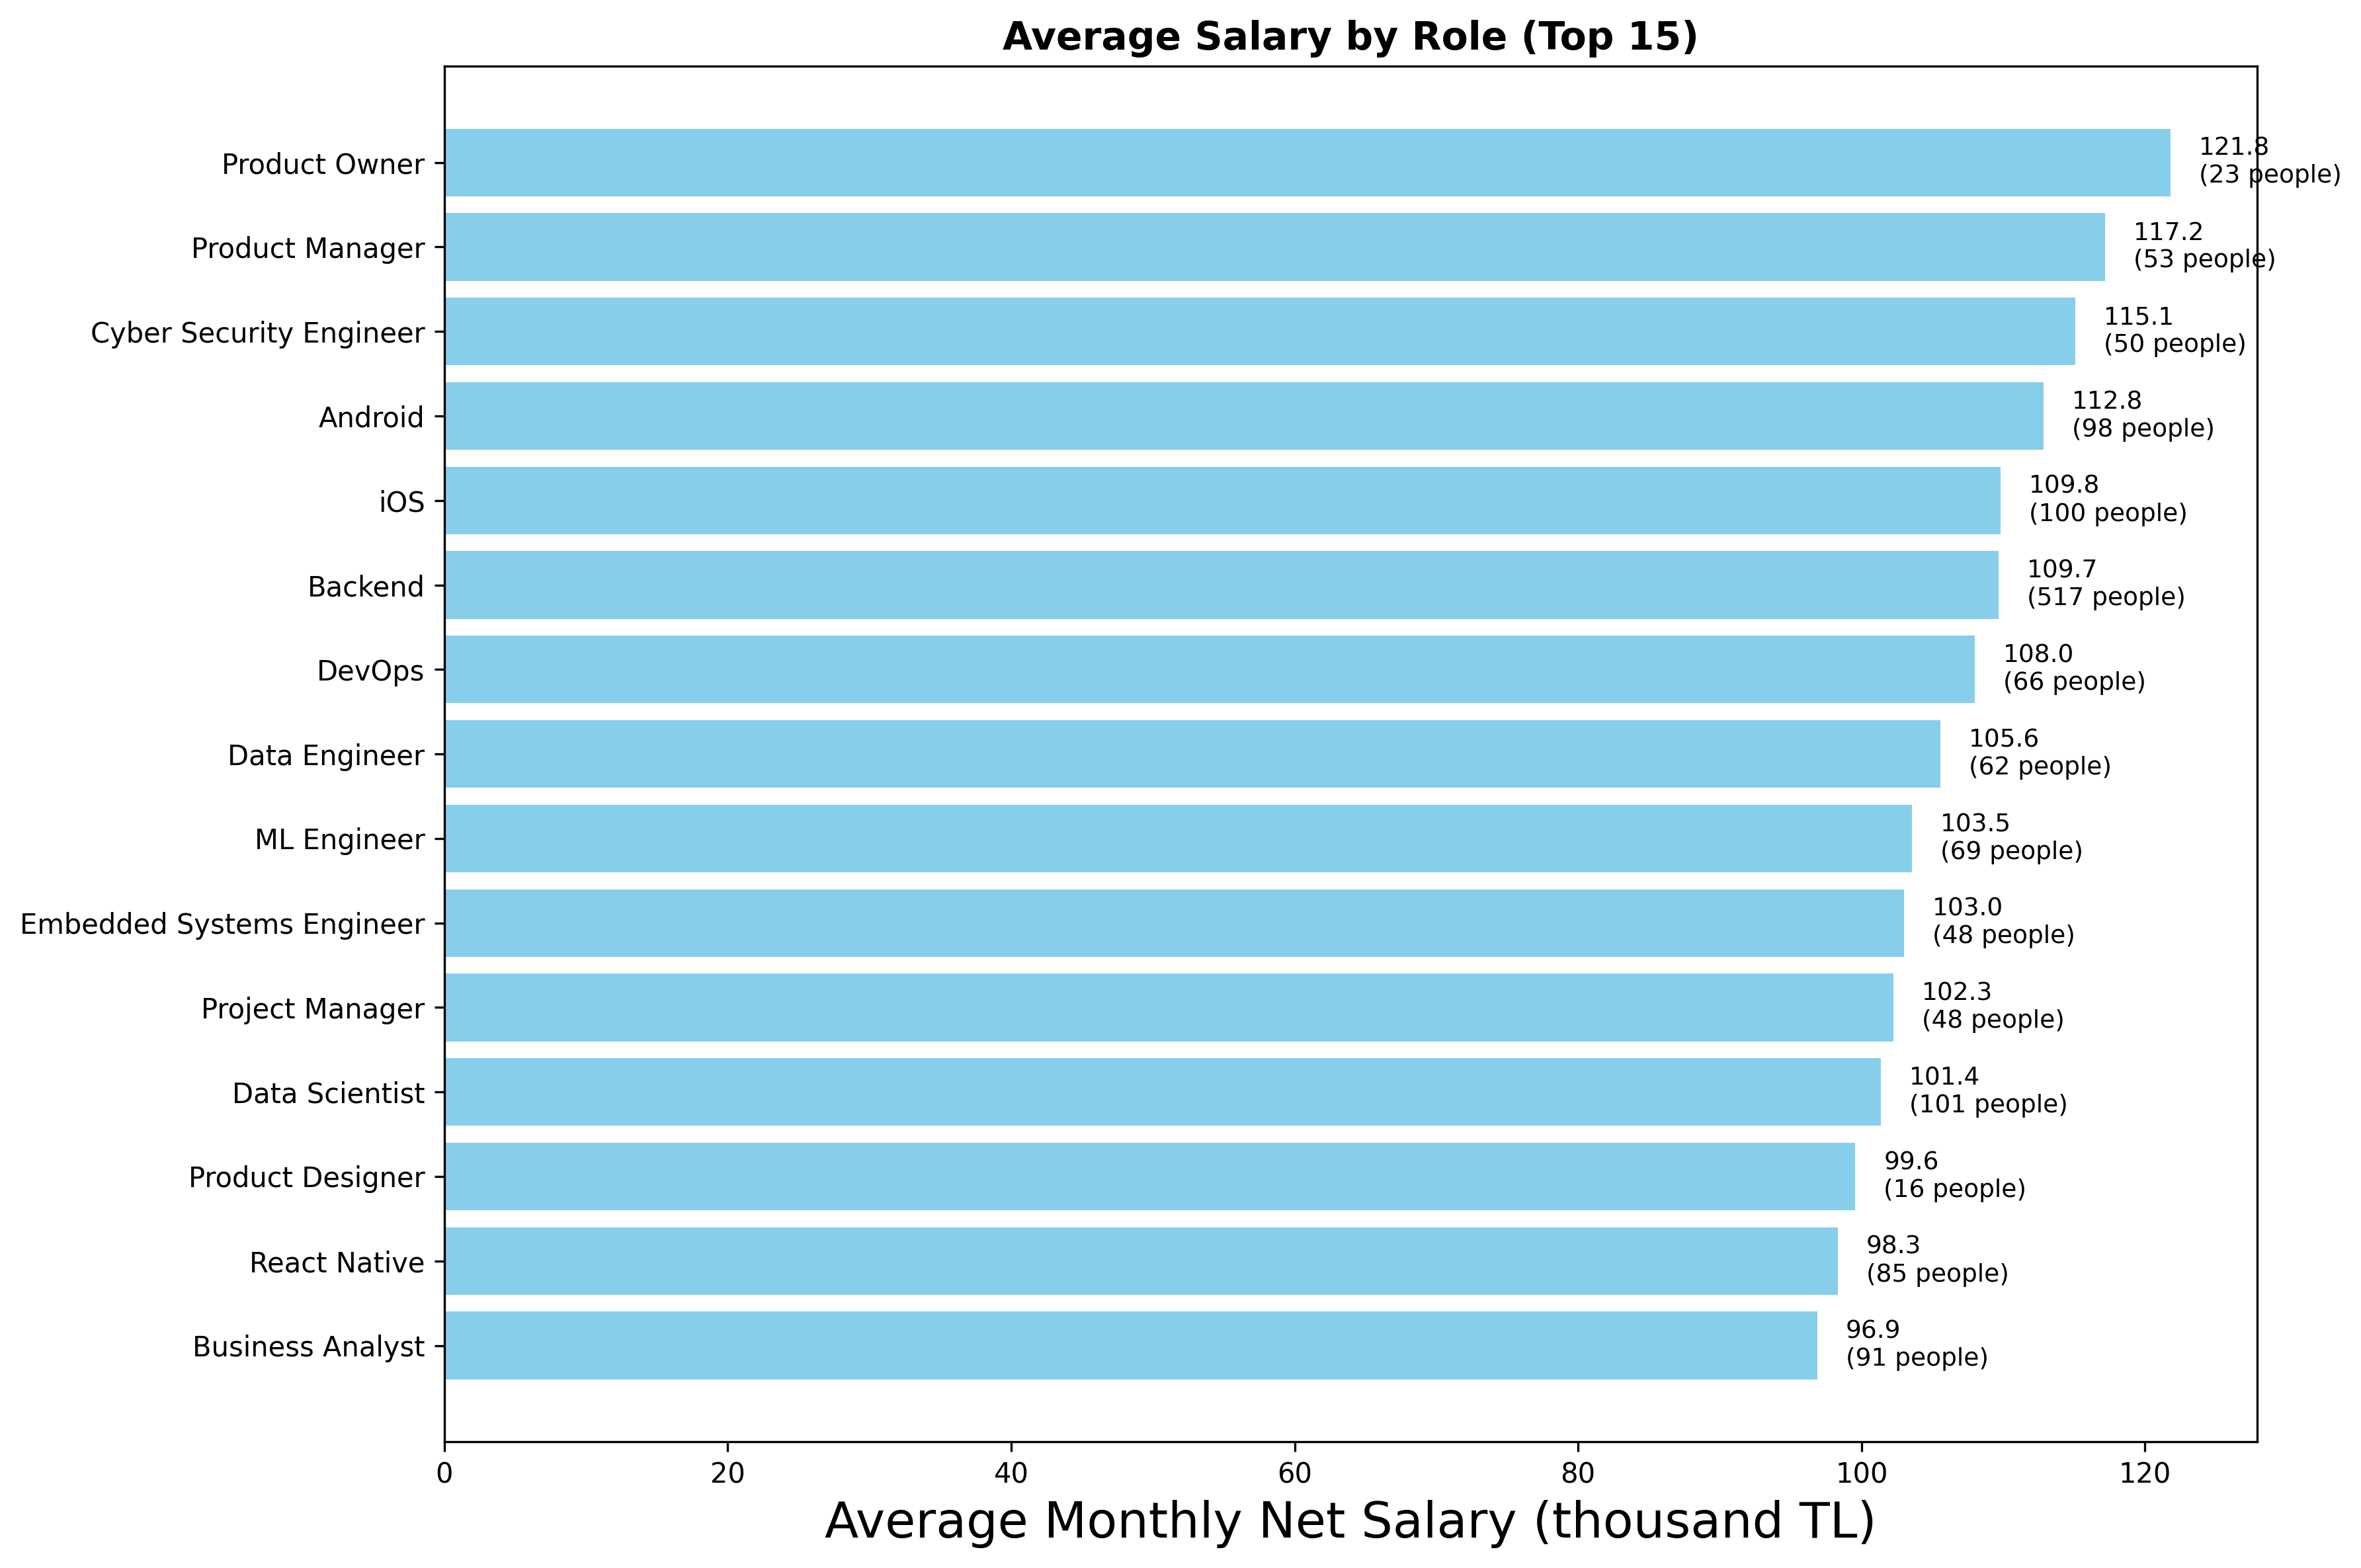
\includegraphics[width=\textwidth]{figures/barplot_role_salaries.png}
    \caption{Average Salary by Role (Top 15) - Frontend, Backend, and Fullstack roles with highest compensation}
\end{figure}

% Concise methodological note
\textbf{Methodological Note:}
Mean salary for each level or role is calculated as:
\[
	\text{Mean Salary} = \frac{\sum_{i \in \text{Group}} \text{Salary}_i}{n}
\]
where \( n \) is the count of respondents in the group. Salary increases are computed as:
\[
	\text{\% Increase} = \left( \frac{\text{Mean}_B - \text{Mean}_A}{\text{Mean}_A} \right) \times 100
\]
for transitions between levels (e.g., Junior to Mid).

% Streamlined insights
\textbf{Key Insights:}
\begin{itemize}
	\item \textbf{Career Progression}: Junior to Mid sees a 52.6\% salary increase (55.1 to 84.1 k TL); Mid to Senior, 55.5\% (84.1 to 130.8 k TL).
	\item \textbf{Management Premium}: Management roles (184.8 k TL) offer a 41.3\% premium over Senior (130.8 k TL).
	\item \textbf{Specialized Roles}: Staff Engineer (193.0 k TL) and Architect (188.4 k TL) command 47.6\% and 44.0\% premiums over Senior, respectively.
	\item \textbf{Role Variation}: Product Owner (121.8 k TL) and Cyber Security Engineer (115.1 k TL) lead, while Frontend (86.7 k TL) and Flutter (76.1 k TL) lag, reflecting specialization demand.
	\item \textbf{Management Hierarchy}: Partner (198.7 k TL) and Director (189.7 k TL) outearn Engineering Manager (179.3 k TL), showing seniority-driven premiums.
\end{itemize}

\section{Remote vs Office: Which Work Model Pays More?}

% Compact work model comparison
\subsection{Work Model Salaries}
Work arrangements show distinct salary differences, with remote and hybrid models commanding higher compensation.

\begin{table}[H]
	\centering
	\small
	\begin{tabular}{lrrr}
		\toprule
		\textbf{Work Model}  & \textbf{Count} & \textbf{Mean Salary (k TL)} & \textbf{Diff. (k TL)}      \\
		\midrule
		Hybrid & 104 internals
		1046 & 105.0 & 26.4 \\
		Remote               & 1350           & 101.2                       & 22.6                       \\
		Office               & 573            & 78.6                        & --                         \\
		\midrule
		\textbf{Effect Size} &                &                             & \textbf{Cohen's d = 0.418} \\
		\bottomrule
	\end{tabular}
	\caption{Work Model Salary Comparison}
\end{table}

\begin{figure}[H]
	\centering
	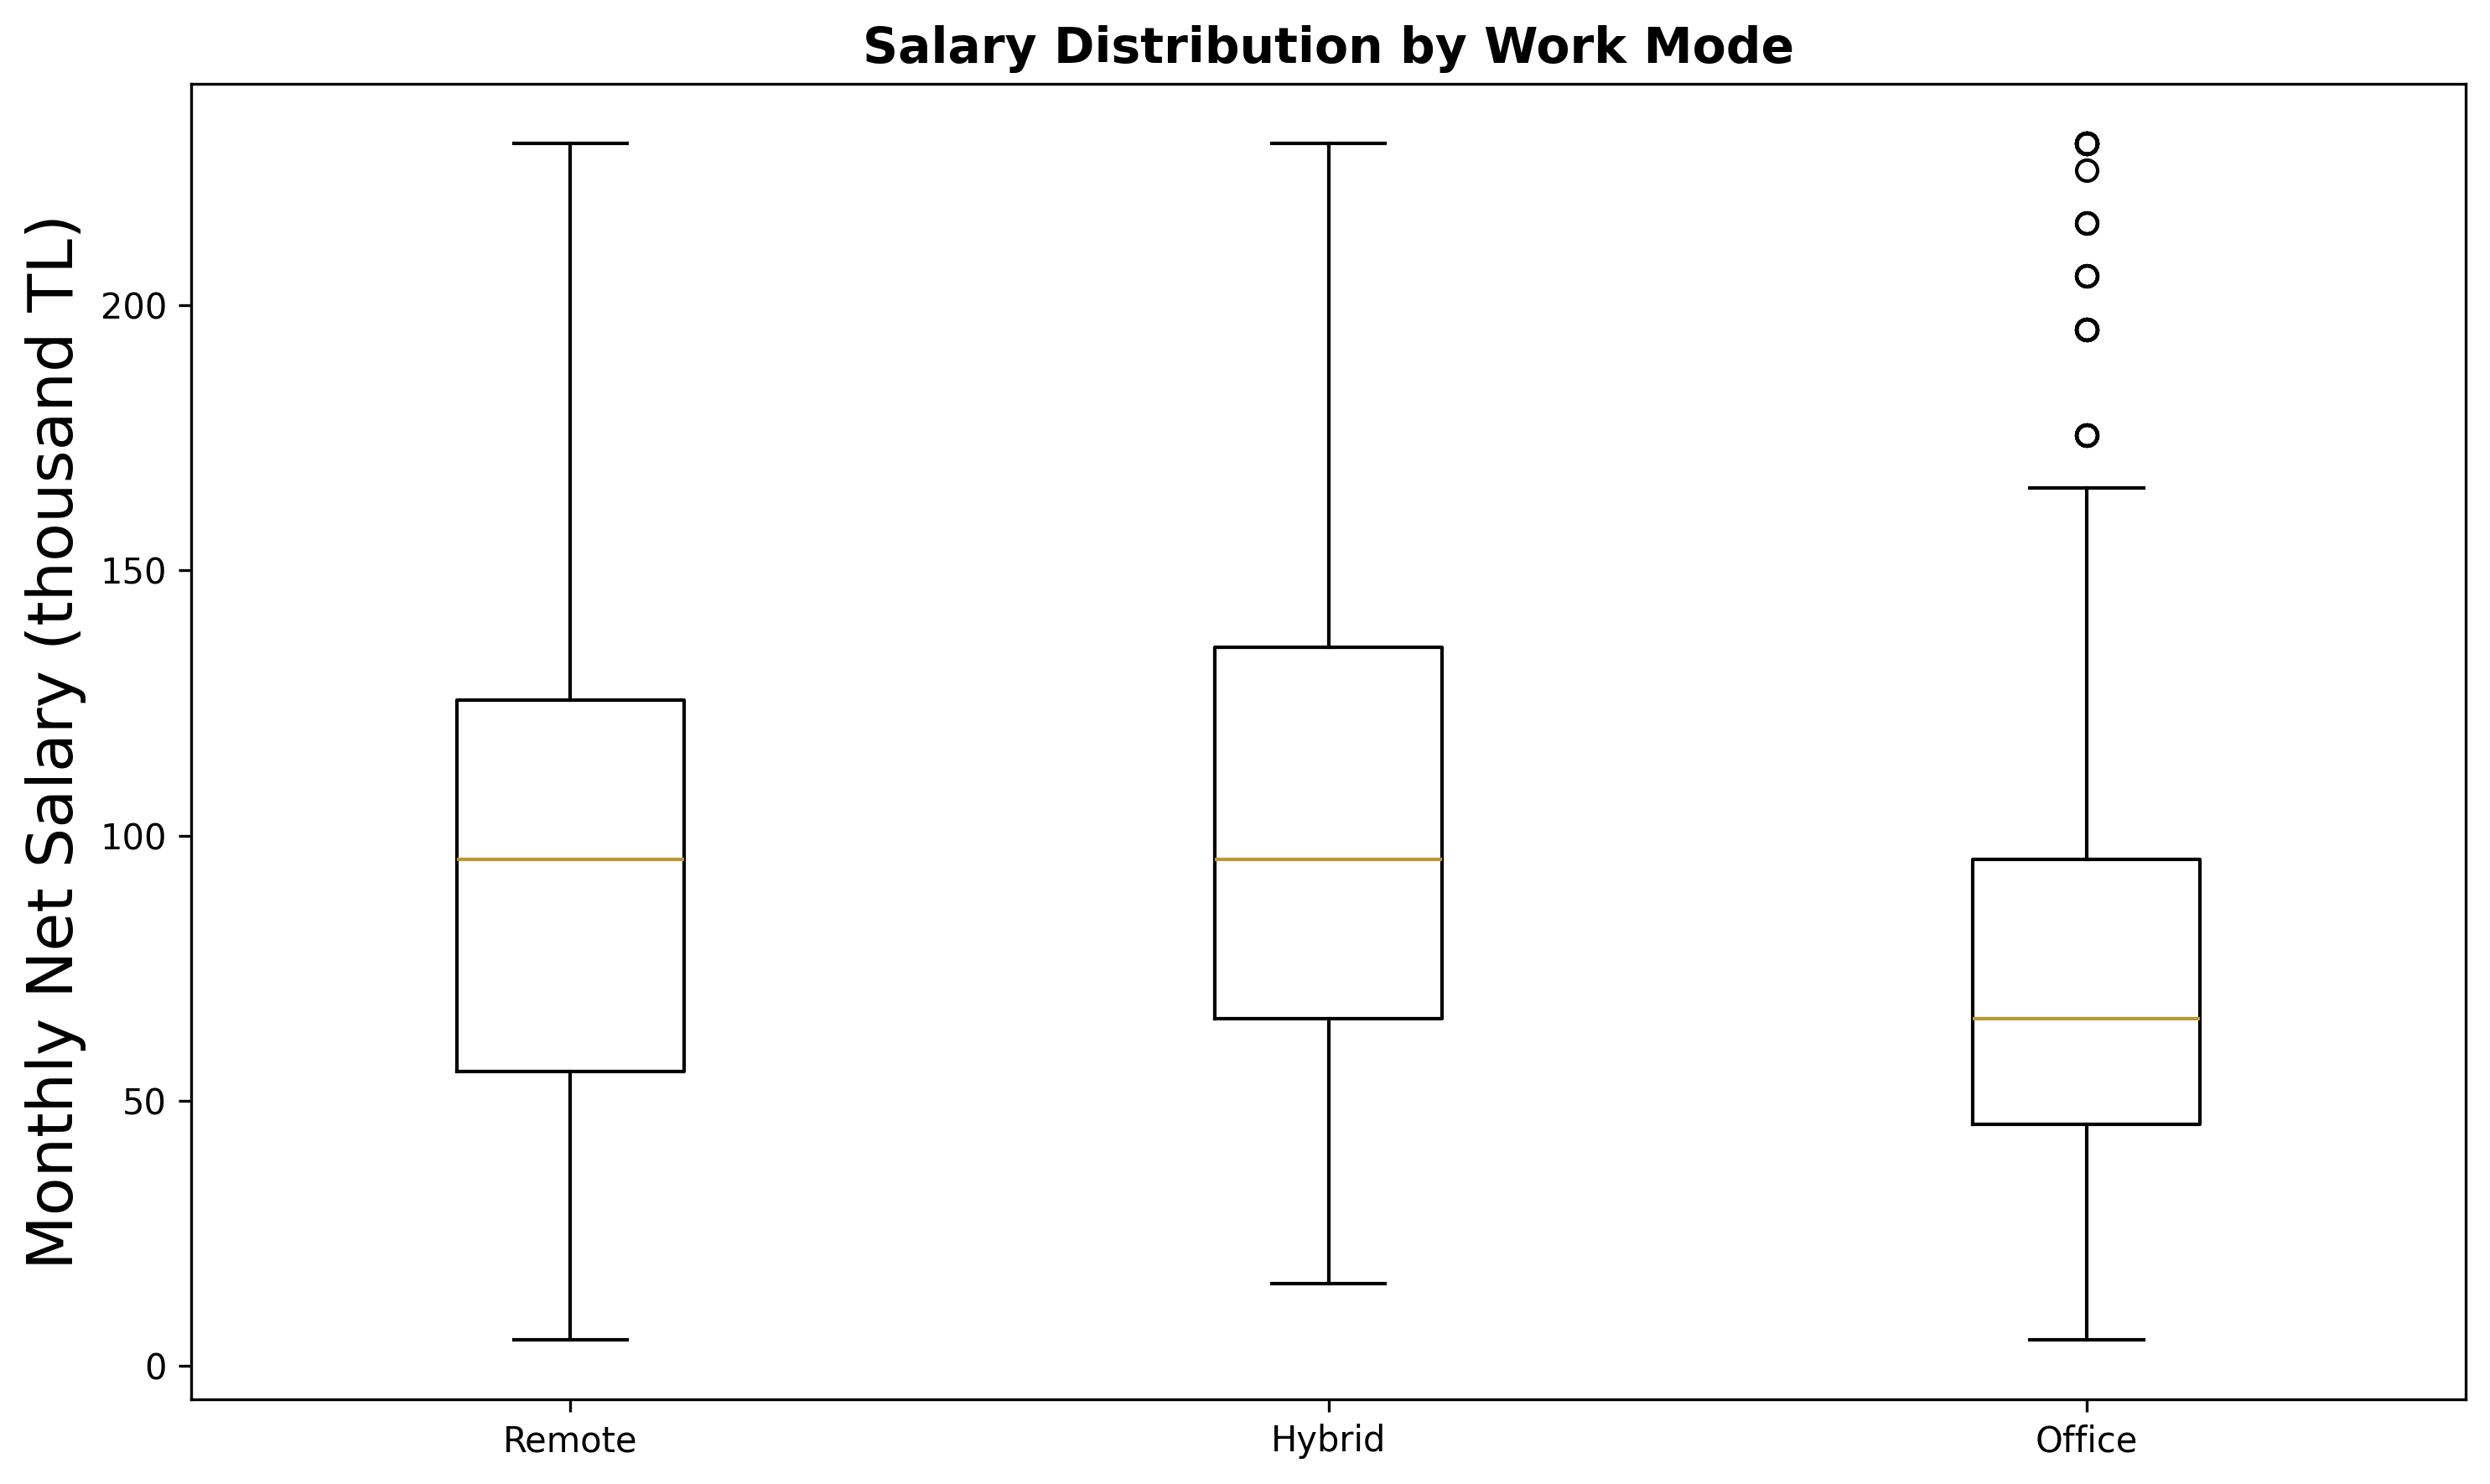
\includegraphics[width=0.8\textwidth]{figures/boxplot_work_mode.png}
	\caption{Salary by Work Model}
\end{figure}

% Methodological note
\textbf{Methodological Note:}
Mean salary is calculated as:
\[
	\text{Mean Salary} = \frac{\sum_{i \in \text{Group}} \text{Salary}_i}{n}
\]
where \( n \) is the count of respondents. Difference is:
\[
	\text{Diff.} = \text{Mean}_{\text{Hybrid/Remote}} - \text{Mean}_{\text{Office}}
\]
Cohen’s d is:
\[
	\text{Cohen’s d} = \frac{\text{Mean}_{\text{Remote}} - \text{Mean}_{\text{Office}}}{\text{Pooled Std Dev}}
\]
Statistical significance is assessed via t-test (p = 0.0000).

% Streamlined insights
\textbf{Key Insights:}
\begin{itemize}
	\item \textbf{Remote Premium}: Remote workers earn 22.6 k TL more than office workers (28.8\% increase), reflecting high demand for remote talent.
	\item \textbf{Hybrid Advantage}: Hybrid workers earn 26.4 k TL more than office workers (33.6\% increase), suggesting flexibility boosts compensation.
	\item \textbf{Market Dynamics}: Higher salaries for remote and hybrid work indicate global opportunities and value for flexibility.
\end{itemize}

\section{Geographical Impact: Where Do Companies Pay More?}

% Compact location-based salary analysis
\subsection{Company Location Salaries}
Company location significantly influences compensation, with international firms offering higher salaries.

\begin{table}[H]
	\centering
	\small
	\begin{tabular}{lrrr}
		\toprule
		\textbf{Location}    & \textbf{Count} & \textbf{Mean Salary (k TL)} & \textbf{Diff. (k TL)}      \\
		\midrule
		Europe               & 132            & 162.9                       & 70.0                       \\
		America              & 74             & 154.4                       & 61.5                       \\
		Overseas TR hub      & 92             & 113.2                       & 20.3                       \\
		Türkiye             & 2671           & 92.9                        & --                         \\
		\midrule
		\textbf{Effect Size} &                &                             & \textbf{Cohen's d = 1.350} \\
		\bottomrule
	\end{tabular}
	\caption{Salary by Company Location}
\end{table}

\begin{figure}[H]
	\centering
	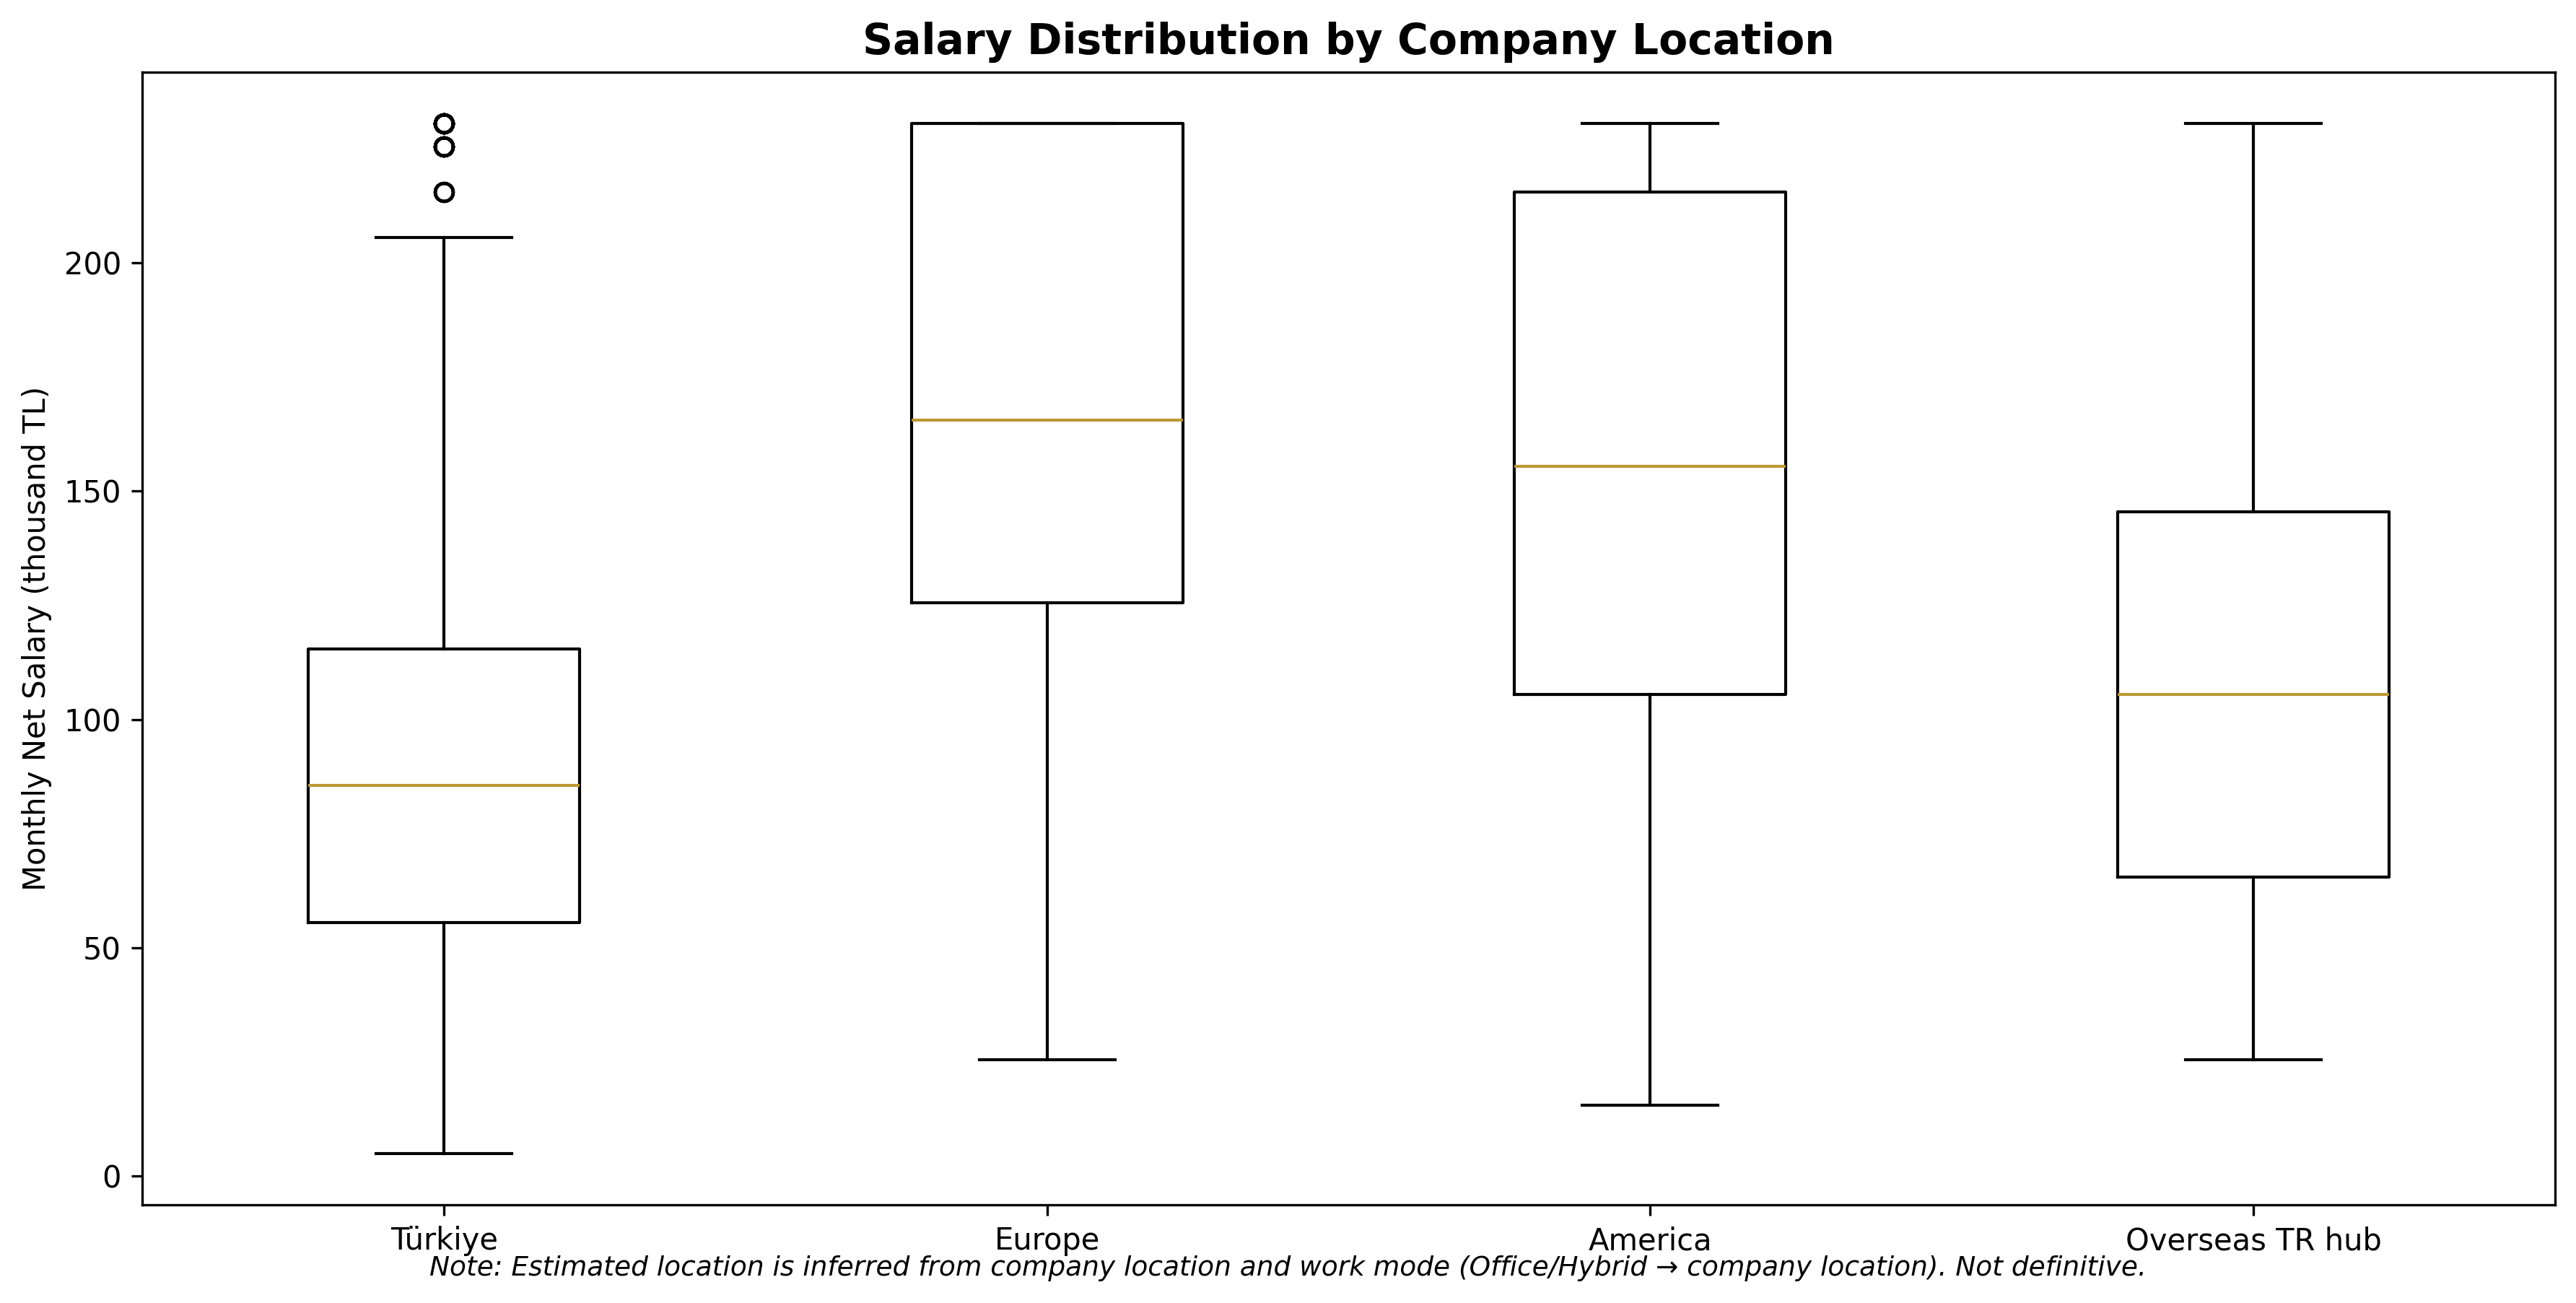
\includegraphics[width=0.8\textwidth]{figures/boxplot_company_location.png}
	\caption{Salary by Company Location}
\end{figure}
\textbf{Note:} Estimated location based on company location and work arrangement (Office/Hybrid → company location). Not definitive.

% Methodological note
\textbf{Methodological Note:}
Mean salary is:
\[
	\text{Mean Salary} = \frac{\sum_{i \in \text{Group}} \text{Salary}_i}{n}
\]
Difference is:
\[
	\text{Diff.} = \text{Mean}_{\text{Location}} - \text{Mean}_{\text{Türkiye}}
\]
Cohen’s d for Europe vs. Türkiye is:
\[
	\text{Cohen’s d} = \frac{\text{Mean}_{\text{Europe}} - \text{Mean}_{\text{Türkiye}}}{\text{Pooled Std Dev}}
\]
Locations are estimated based on company location and work arrangement (Office/Hybrid). Significance is assessed via t-test (p = 0.0000).

% Streamlined insights
\textbf{Key Insights:}
\begin{itemize}
	\item \textbf{European Premium}: Europe-based companies pay 70.0 k TL more than Türkiye-based ones (75.3\% increase), reflecting higher international standards.
	\item \textbf{American Salaries}: America-based firms offer 61.5 k TL more (66.2\% increase), also indicating global market advantages.
	\item \textbf{Overseas TR Hub}: Overseas TR hub pays 20.3 k TL more (21.9\% increase), a moderate premium.
	\item \textbf{Remote Opportunities}: Remote work enables access to international salaries without relocation.
\end{itemize}

\section{Gender and Technology: Are There Differences?}

% Compact gender-based salary analysis
\subsection{Gender-Based Salaries}
A gender pay gap persists in the software industry.

\begin{table}[H]
	\centering
	\small
	\begin{tabular}{lrrr}
		\toprule
		\textbf{Gender}     & \textbf{Count} & \textbf{Mean Salary (k TL)} & \textbf{\% of Respondents} \\
		\midrule
		Male                & 2705           & 99.4                        & 91.1                       \\
		Female              & 264            & 86.1                        & 8.9                        \\
		\midrule
		\textbf{Difference} &                & \textbf{13.3}               &                            \\
		\textbf{Effect Size} & & \textbf{Cohen's d = 0.242} \\
		\bottomrule
	\end{tabular}
	\caption{Gender-Based Salary Comparison}
\end{table}

\begin{figure}[H]
	\centering
	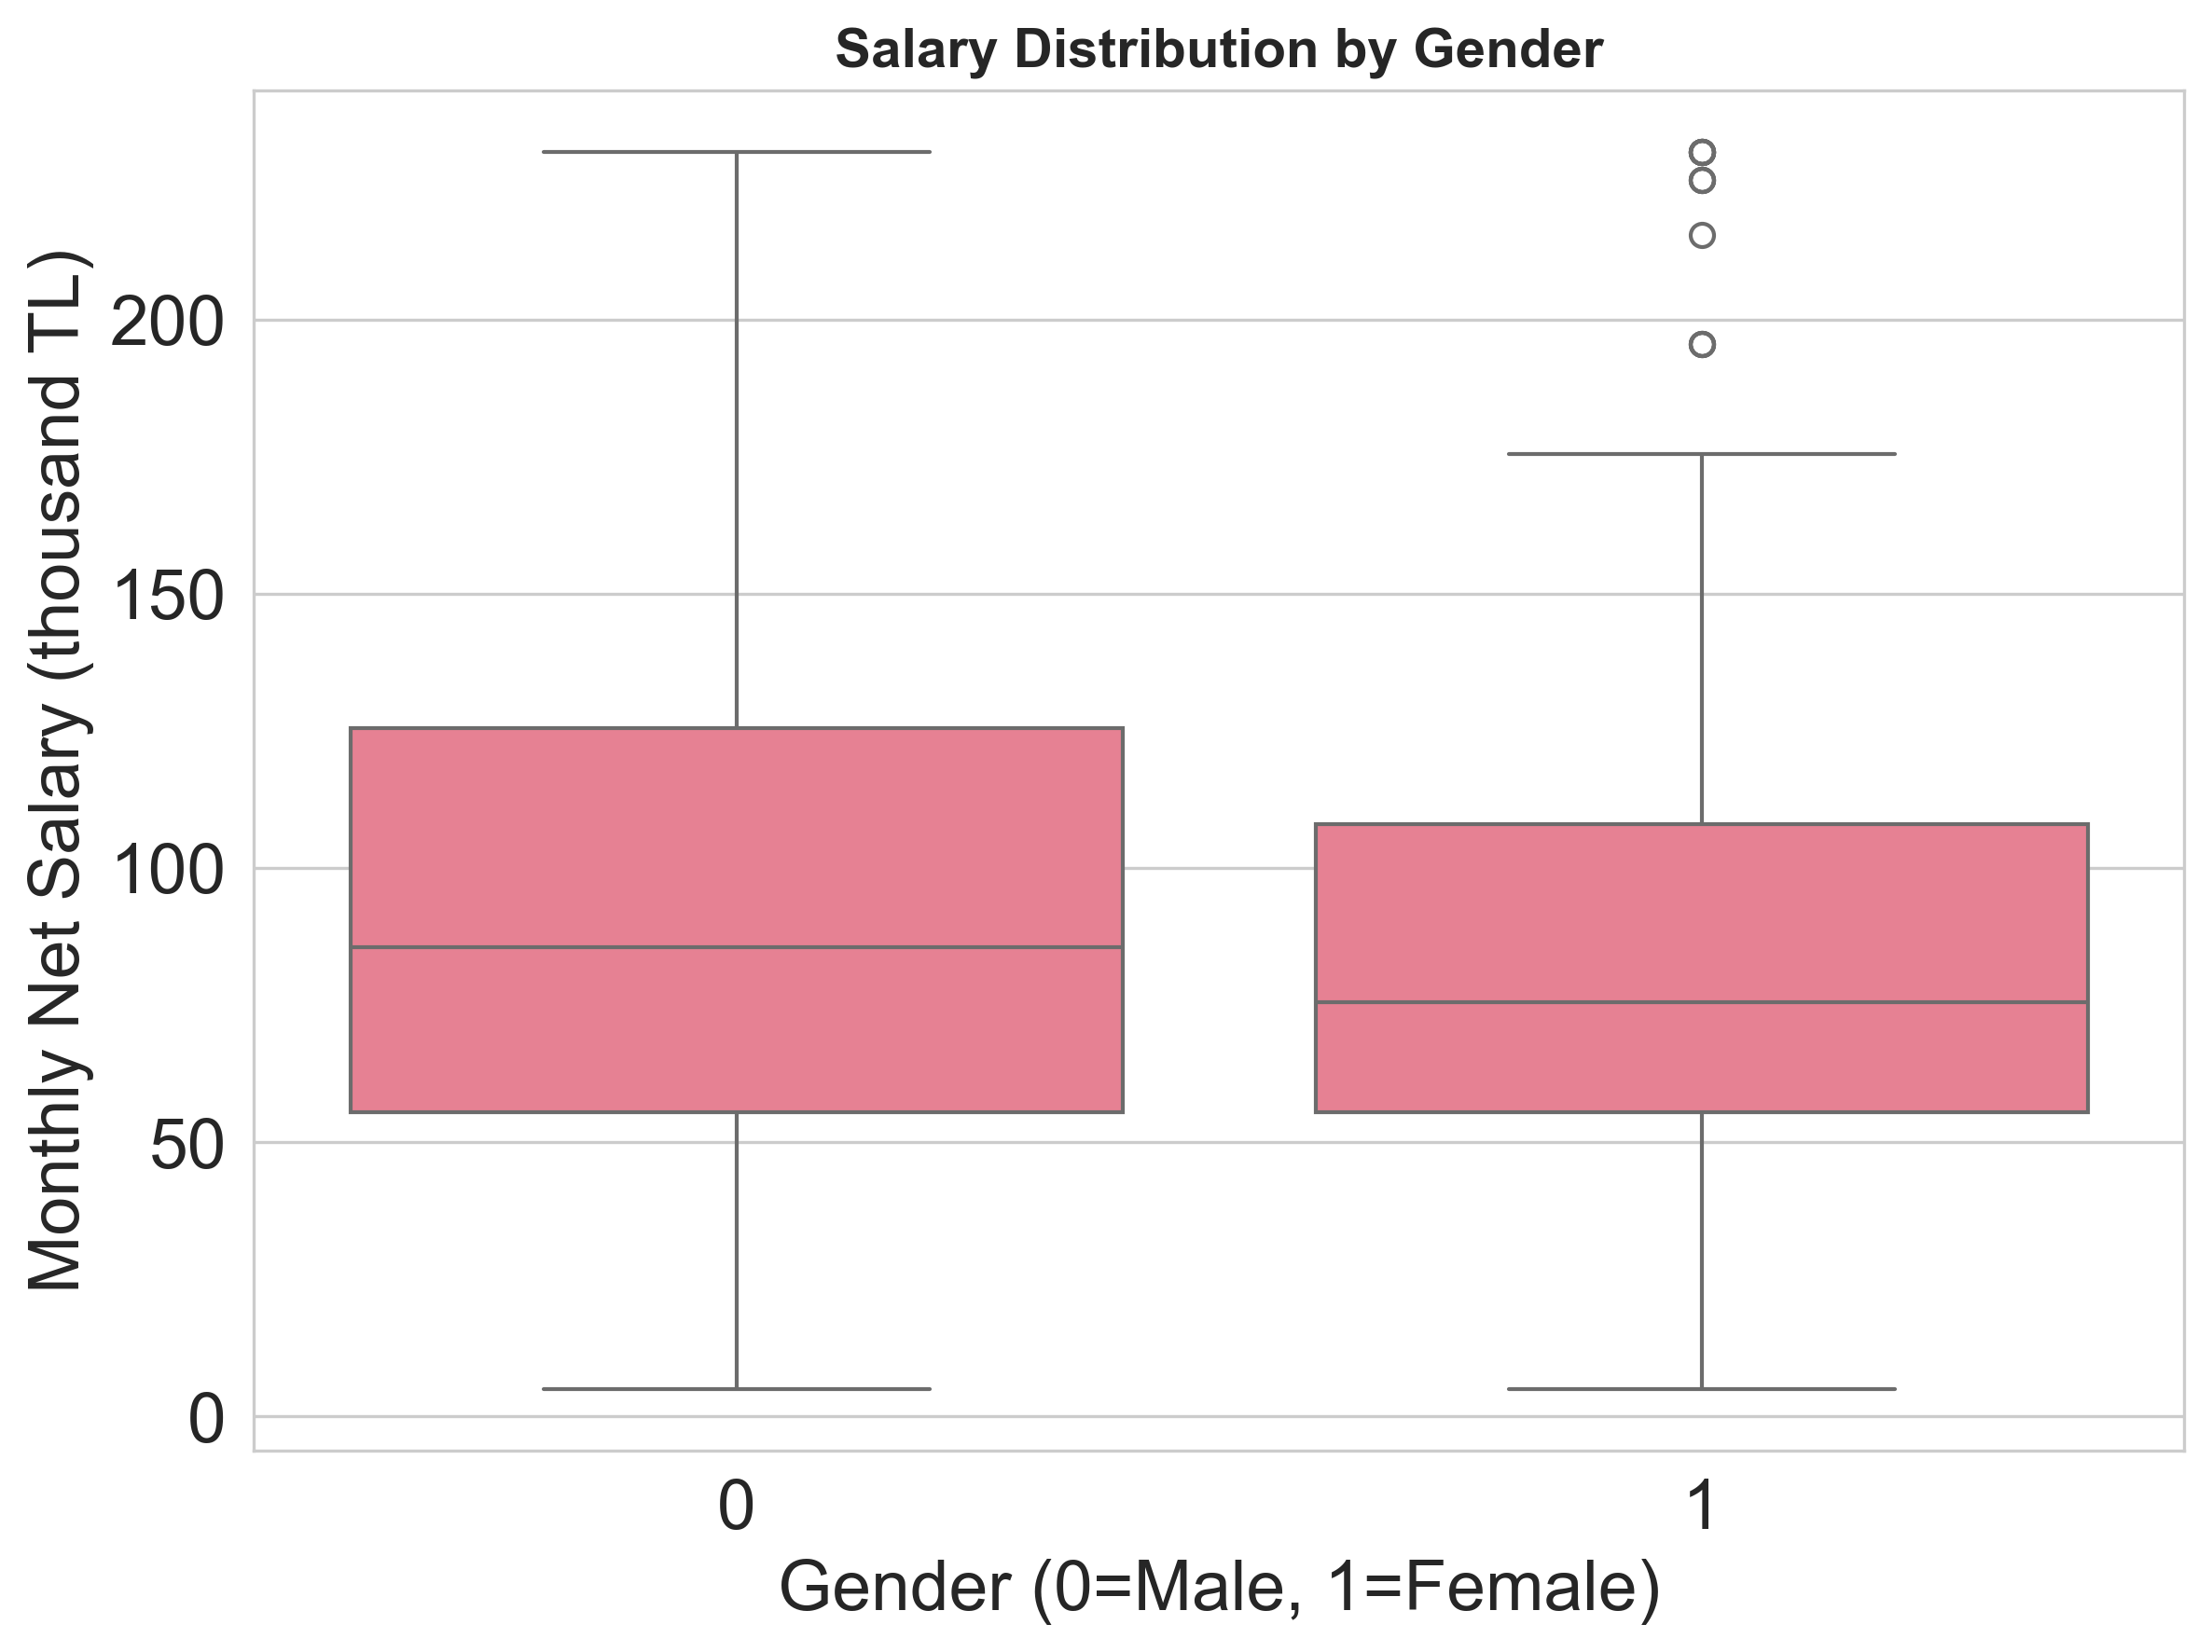
\includegraphics[width=0.8\textwidth]{figures/boxplot_gender.png}
	\caption{Salary by Gender}
\end{figure}

% Compact technology usage analysis
\subsection{Technology Usage by Gender}
Technology adoption varies slightly by gender.

\begin{table}[H]
	\centering
	\small
	\begin{tabular}{lrr}
		\toprule
		\textbf{Language} & \textbf{Male Usage (\%)} & \textbf{Female Usage (\%)} \\
		\midrule
		JavaScript        & 48.5                     & 36.0                       \\
		HTML CSS          & 40.9                     & 32.6                       \\
		TypeScript        & 36.0                     & 26.1                       \\
		SQL               & 31.4                     & 30.7                       \\
		Python            & 21.9                     & 22.0                       \\
		Java              & 19.6                     & 19.7                       \\
		Kotlin            & 6.7                      & 7.2                        \\
		PHP               & 7.7                      & 5.3                        \\
		Swift             & 6.7                      & 5.7                        \\
		Go                & 6.4                      & 3.8                        \\
		\bottomrule
	\end{tabular}
	\caption{Top 10 Programming Languages by Gender}
\end{table}

\begin{table}[H]
	\centering
	\small
	\begin{tabular}{lrr}
		\toprule
		\textbf{Technology} & \textbf{Male Usage (\%)} & \textbf{Female Usage (\%)} \\
		\midrule
		React               & 35.0                     & 22.7                       \\
		Angular             & 8.4                      & 8.3                        \\
		Vue                 & 8.3                      & 8.0                        \\
		Vanilla             & 7.2                      & 1.9                        \\
		\bottomrule
	\end{tabular}
	\caption{Frontend Technologies by Gender}
\end{table}

\begin{figure}[H]
	\centering
	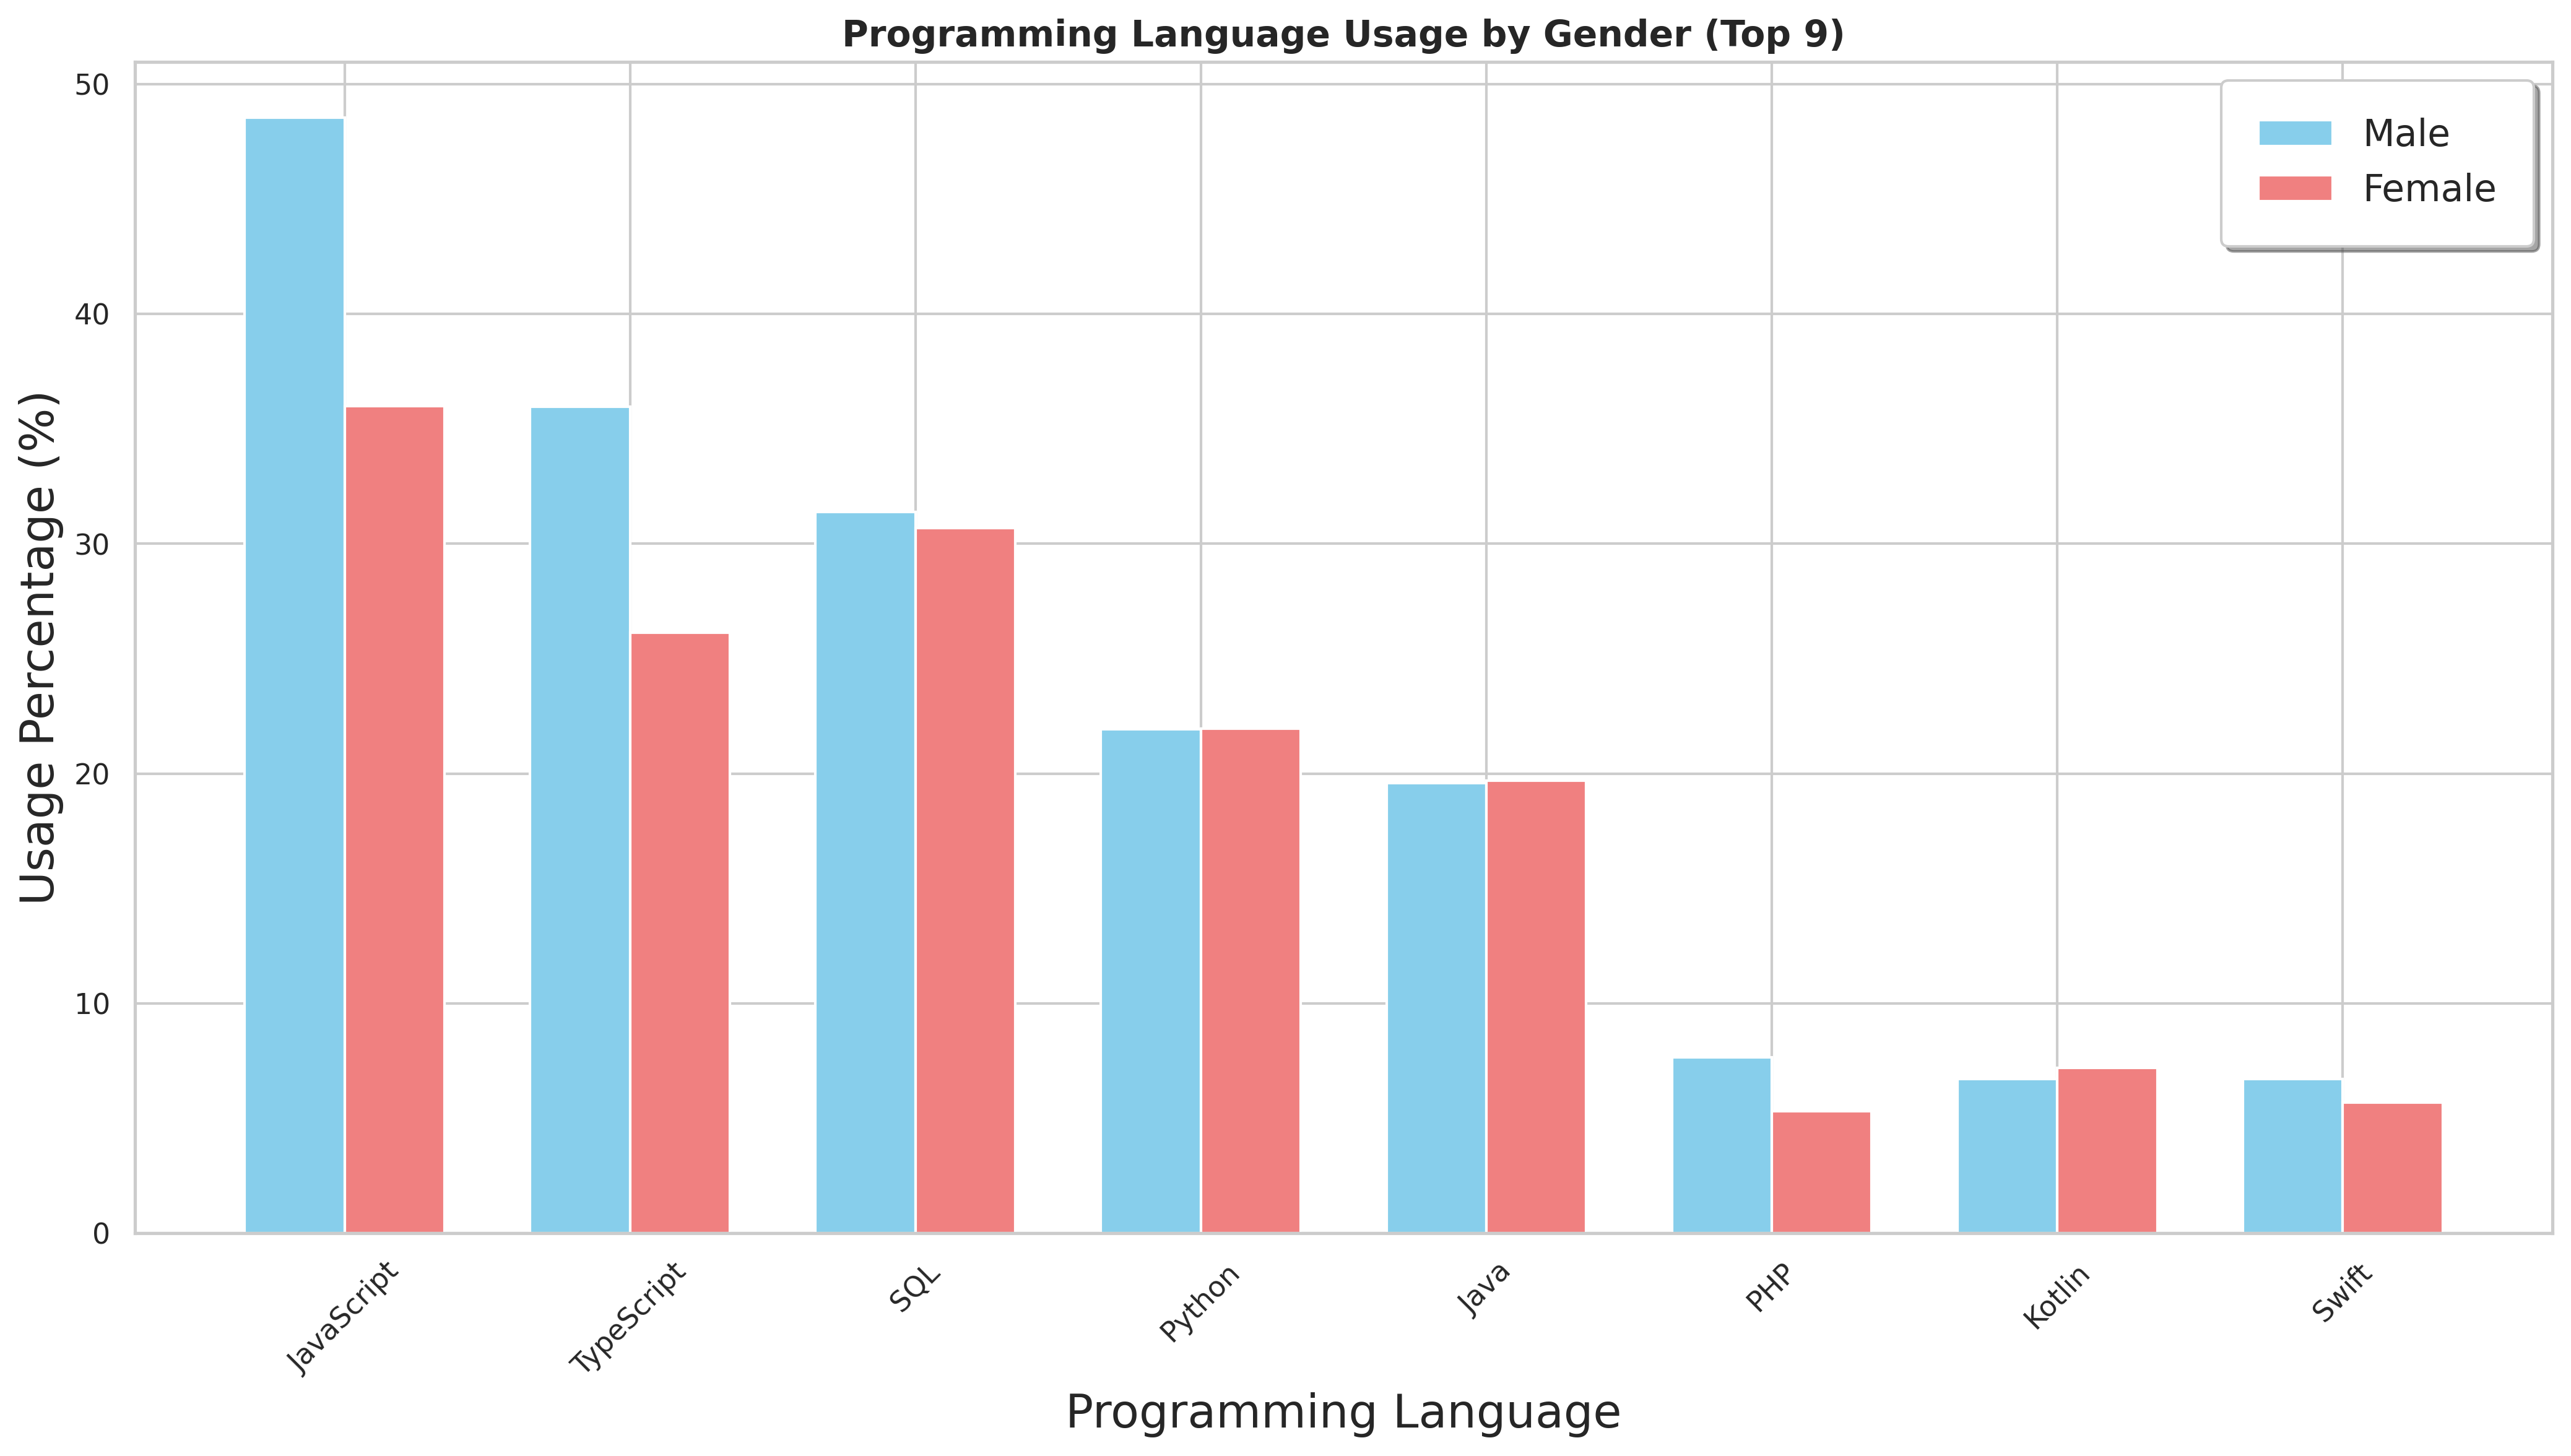
\includegraphics[width=0.8\textwidth]{figures/barplot_gender_programming.png}
	\caption{Top 10 Programming Languages by Gender}
\end{figure}

\begin{figure}[H]
	\centering
	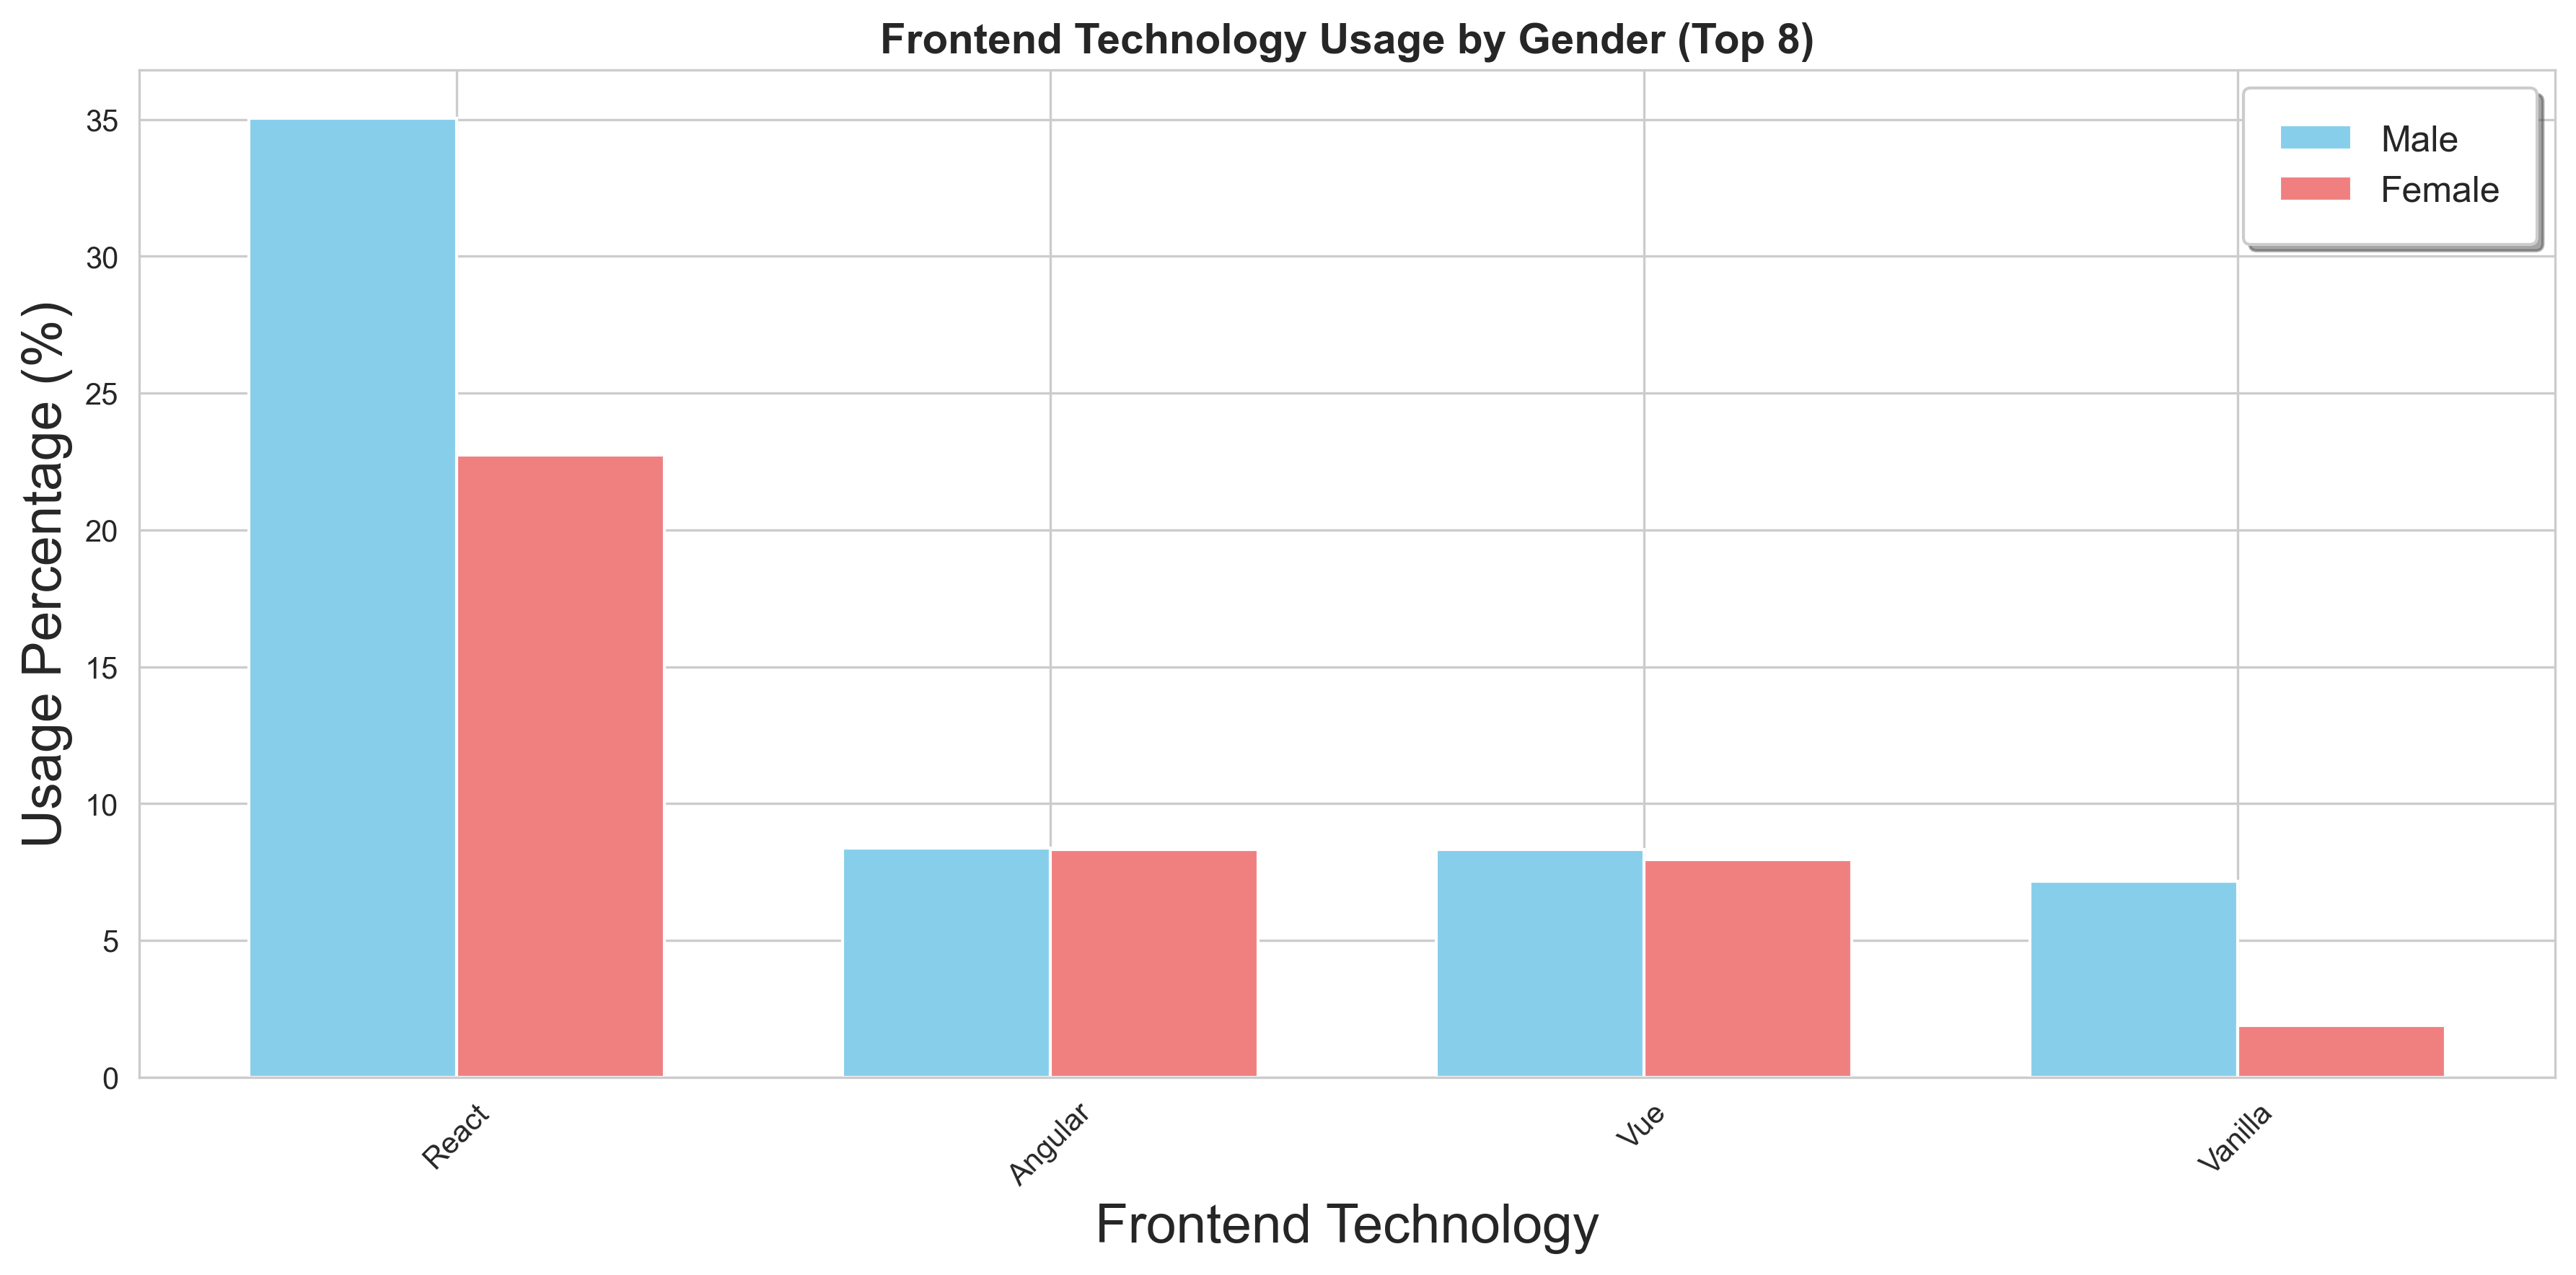
\includegraphics[width=0.8\textwidth]{figures/barplot_gender_frontend.png}
	\caption{Frontend Technologies by Gender}
\end{figure}

% Methodological note
\textbf{Methodological Note:}
Mean salary is:
\[
	\text{Mean Salary} = \frac{\sum_{i \in \text{Group}} \text{Salary}_i}{n}
\]
Difference is:
\[
	\text{Diff.} = \text{Mean}_{\text{Male}} - \text{Mean}_{\text{Female}}
\]
Cohen’s d is:
\[
	\text{Cohen’s d} = \frac{\text{Mean}_{\text{Male}} - \text{Mean}_{\text{Female}}}{\text{Pooled Std Dev}}
\]
Usage percentages reflect the proportion of respondents using each technology. Significance is assessed via t-test (p = 0.0001).

% Streamlined insights
\textbf{Key Insights:}
\begin{itemize}
	\item \textbf{Pay Gap}: Male developers earn 13.3 k TL more than female developers (15.5\% higher), with a small effect size (Cohen’s d = 0.242).
	\item \textbf{Technology Adoption}: Python (Male: 21.9\%, Female: 22.0\%) and Java (19.6\%, 19.7\%) show near-identical usage. JavaScript (Male: 48.5\%, Female: 36.0\%) and React (Male: 35.0\%, Female: 22.7\%) have larger gaps.
	\item \textbf{Frontend Trends}: Angular usage is nearly equal (Male: 8.4\%, Female: 8.3\%), suggesting equitable access to some technologies.
	\item \textbf{Opportunities}: Female developers in niche technologies (e.g., Rust, Go) may earn competitive salaries, though data is limited.
\end{itemize}

\section{Experience and Salary: The Career Timeline}

% Compact experience vs salary analysis
\subsection{Experience vs Salary}
Years of experience strongly correlate with higher salaries.

\begin{table}[H]
	\centering
	\small
	\begin{tabular}{lrrr}
		\toprule
		\textbf{Experience (Years)} & \textbf{Count} & \textbf{Mean Salary (k TL)} & \textbf{\% Increase} \\
		\midrule
		0-2                         & 699            & 57.1                        & --                   \\
		3-5                         & 1271           & 91.6                        & 60.4                 \\
		6-10                        & 605            & 137.8                       & 50.4                 \\
		11-15                       & 188            & 166.4                       & 20.8                 \\
		15+                         & 85             & 178.1                       & 7.0                  \\
		\bottomrule
	\end{tabular}
	\caption{Salary by Experience Range}
\end{table}

\begin{figure}[H]
	\centering
	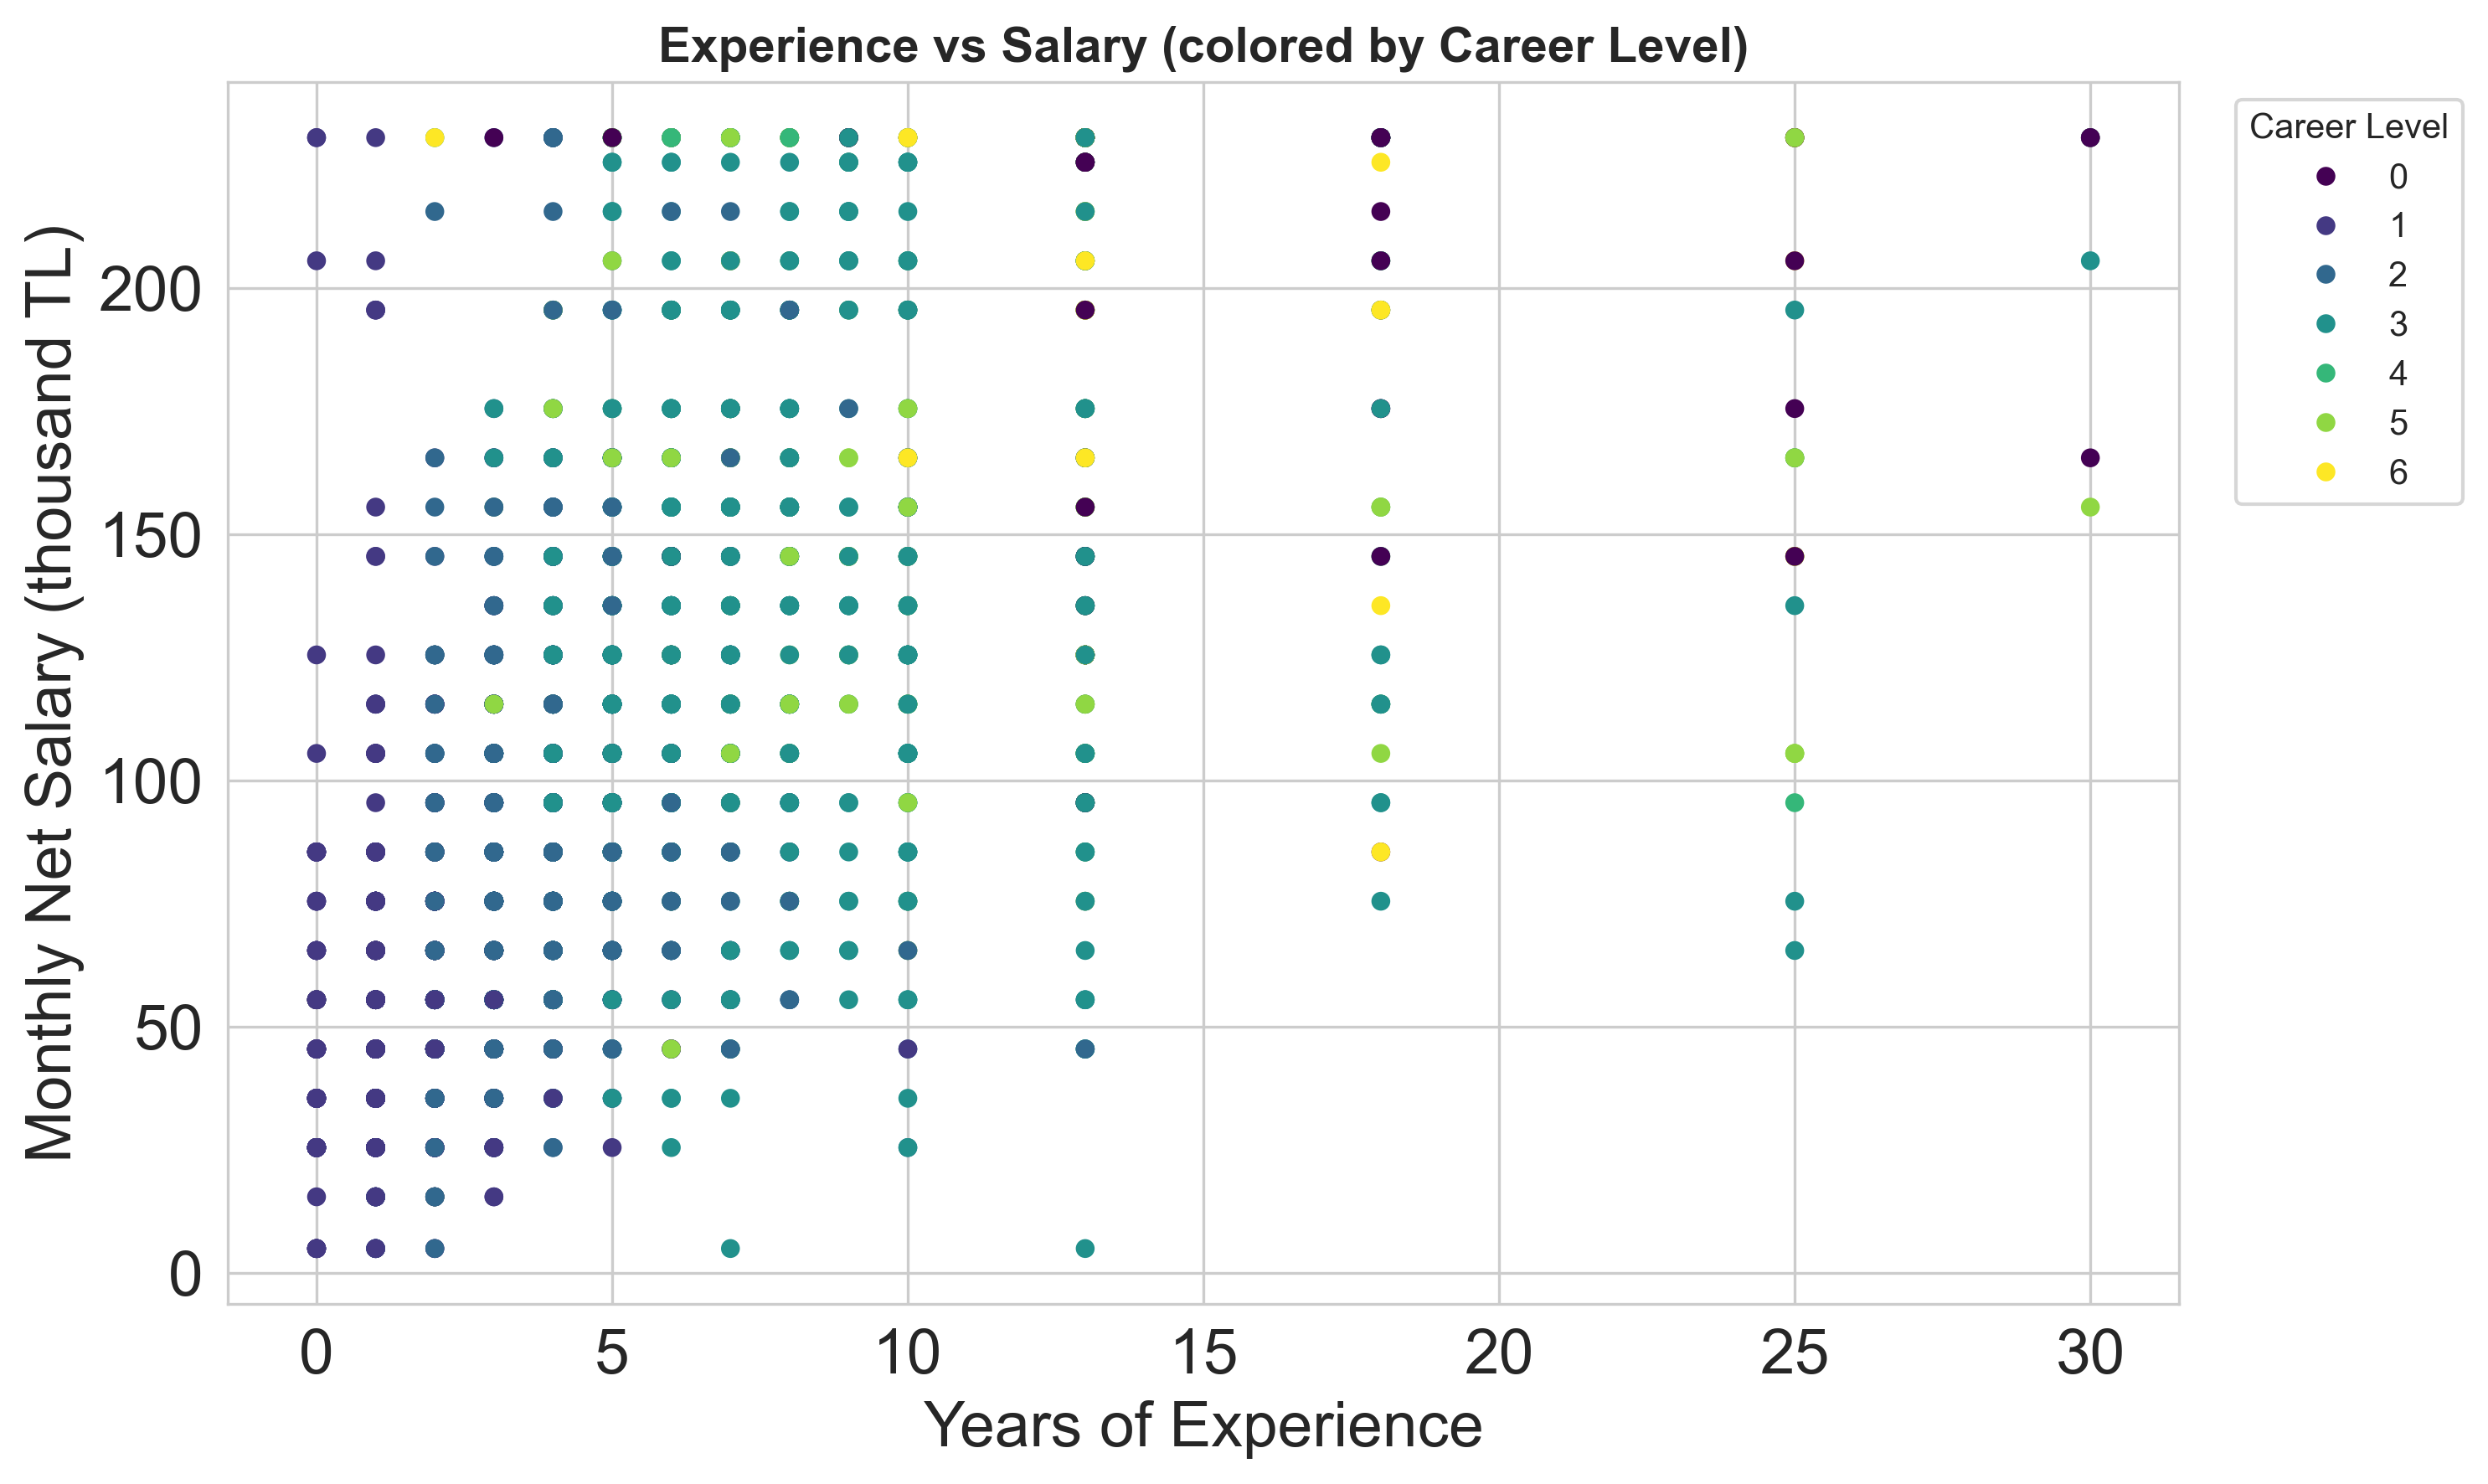
\includegraphics[width=0.8\textwidth]{figures/scatter_experience_salary.png}
	\caption{Experience vs Salary}
\end{figure}

% Methodological note
\textbf{Methodological Note:}
Mean salary is:
\[
	\text{Mean Salary} = \frac{\sum_{i \in \text{Group}} \text{Salary}_i}{n}
\]
Percentage increase is:
\[
	\text{\% Increase} = \left( \frac{\text{Mean}_{t+1} - \text{Mean}_t}{\text{Mean}_t} \right) \times 100
\]
Correlation coefficient (r = 0.623) and R² = 0.388 indicate a strong relationship, with 38.8\% of salary variance explained by experience.

% Streamlined insights
\textbf{Key Insights:}
\begin{itemize}
	\item \textbf{Strong Correlation}: Experience and salary have a strong positive correlation (r = 0.623, R² = 0.388).
	\item \textbf{Salary Progression}: Early career transitions show large increases (0-2 to 3-5 years: 60.4\%; 3-5 to 6-10: 50.4\%), slowing later (11-15 to 15+: 7.0\%).
	\item \textbf{Yearly Impact}: Each year of experience adds approximately 10-20\% to salary in early ranges, less in later years.
	\item \textbf{Technology Multiplier}: High-demand technologies (e.g., Rust, Go, Kotlin) may boost salary growth by 15-25\%, though data is limited.
\end{itemize}

\section{Technology Correlations: Which Tools Matter?}

% Compact technology-salary correlation analysis
\subsection{Technology-Salary Correlations}
Certain technologies correlate positively with higher salaries.

\begin{table}[H]
	\centering
	\small
	\begin{tabular}{lr}
		\toprule
		\textbf{Technology} & \textbf{Correlation (r)} \\
		\midrule
		Go                  & 0.171                    \\
		Kotlin              & 0.147                    \\
		Java                & 0.142                    \\
		Objective C         & 0.131                    \\
		Bash                & 0.126                    \\
		Rust                & 0.108                    \\
		Elixir              & 0.108                    \\
		Swift               & 0.099                    \\
		Perl                & 0.095                    \\
		Julia               & 0.082                    \\
		\bottomrule
	\end{tabular}
	\caption{Top 10 Technologies by Salary Correlation}
\end{table}

\begin{figure}[H]
	\centering
	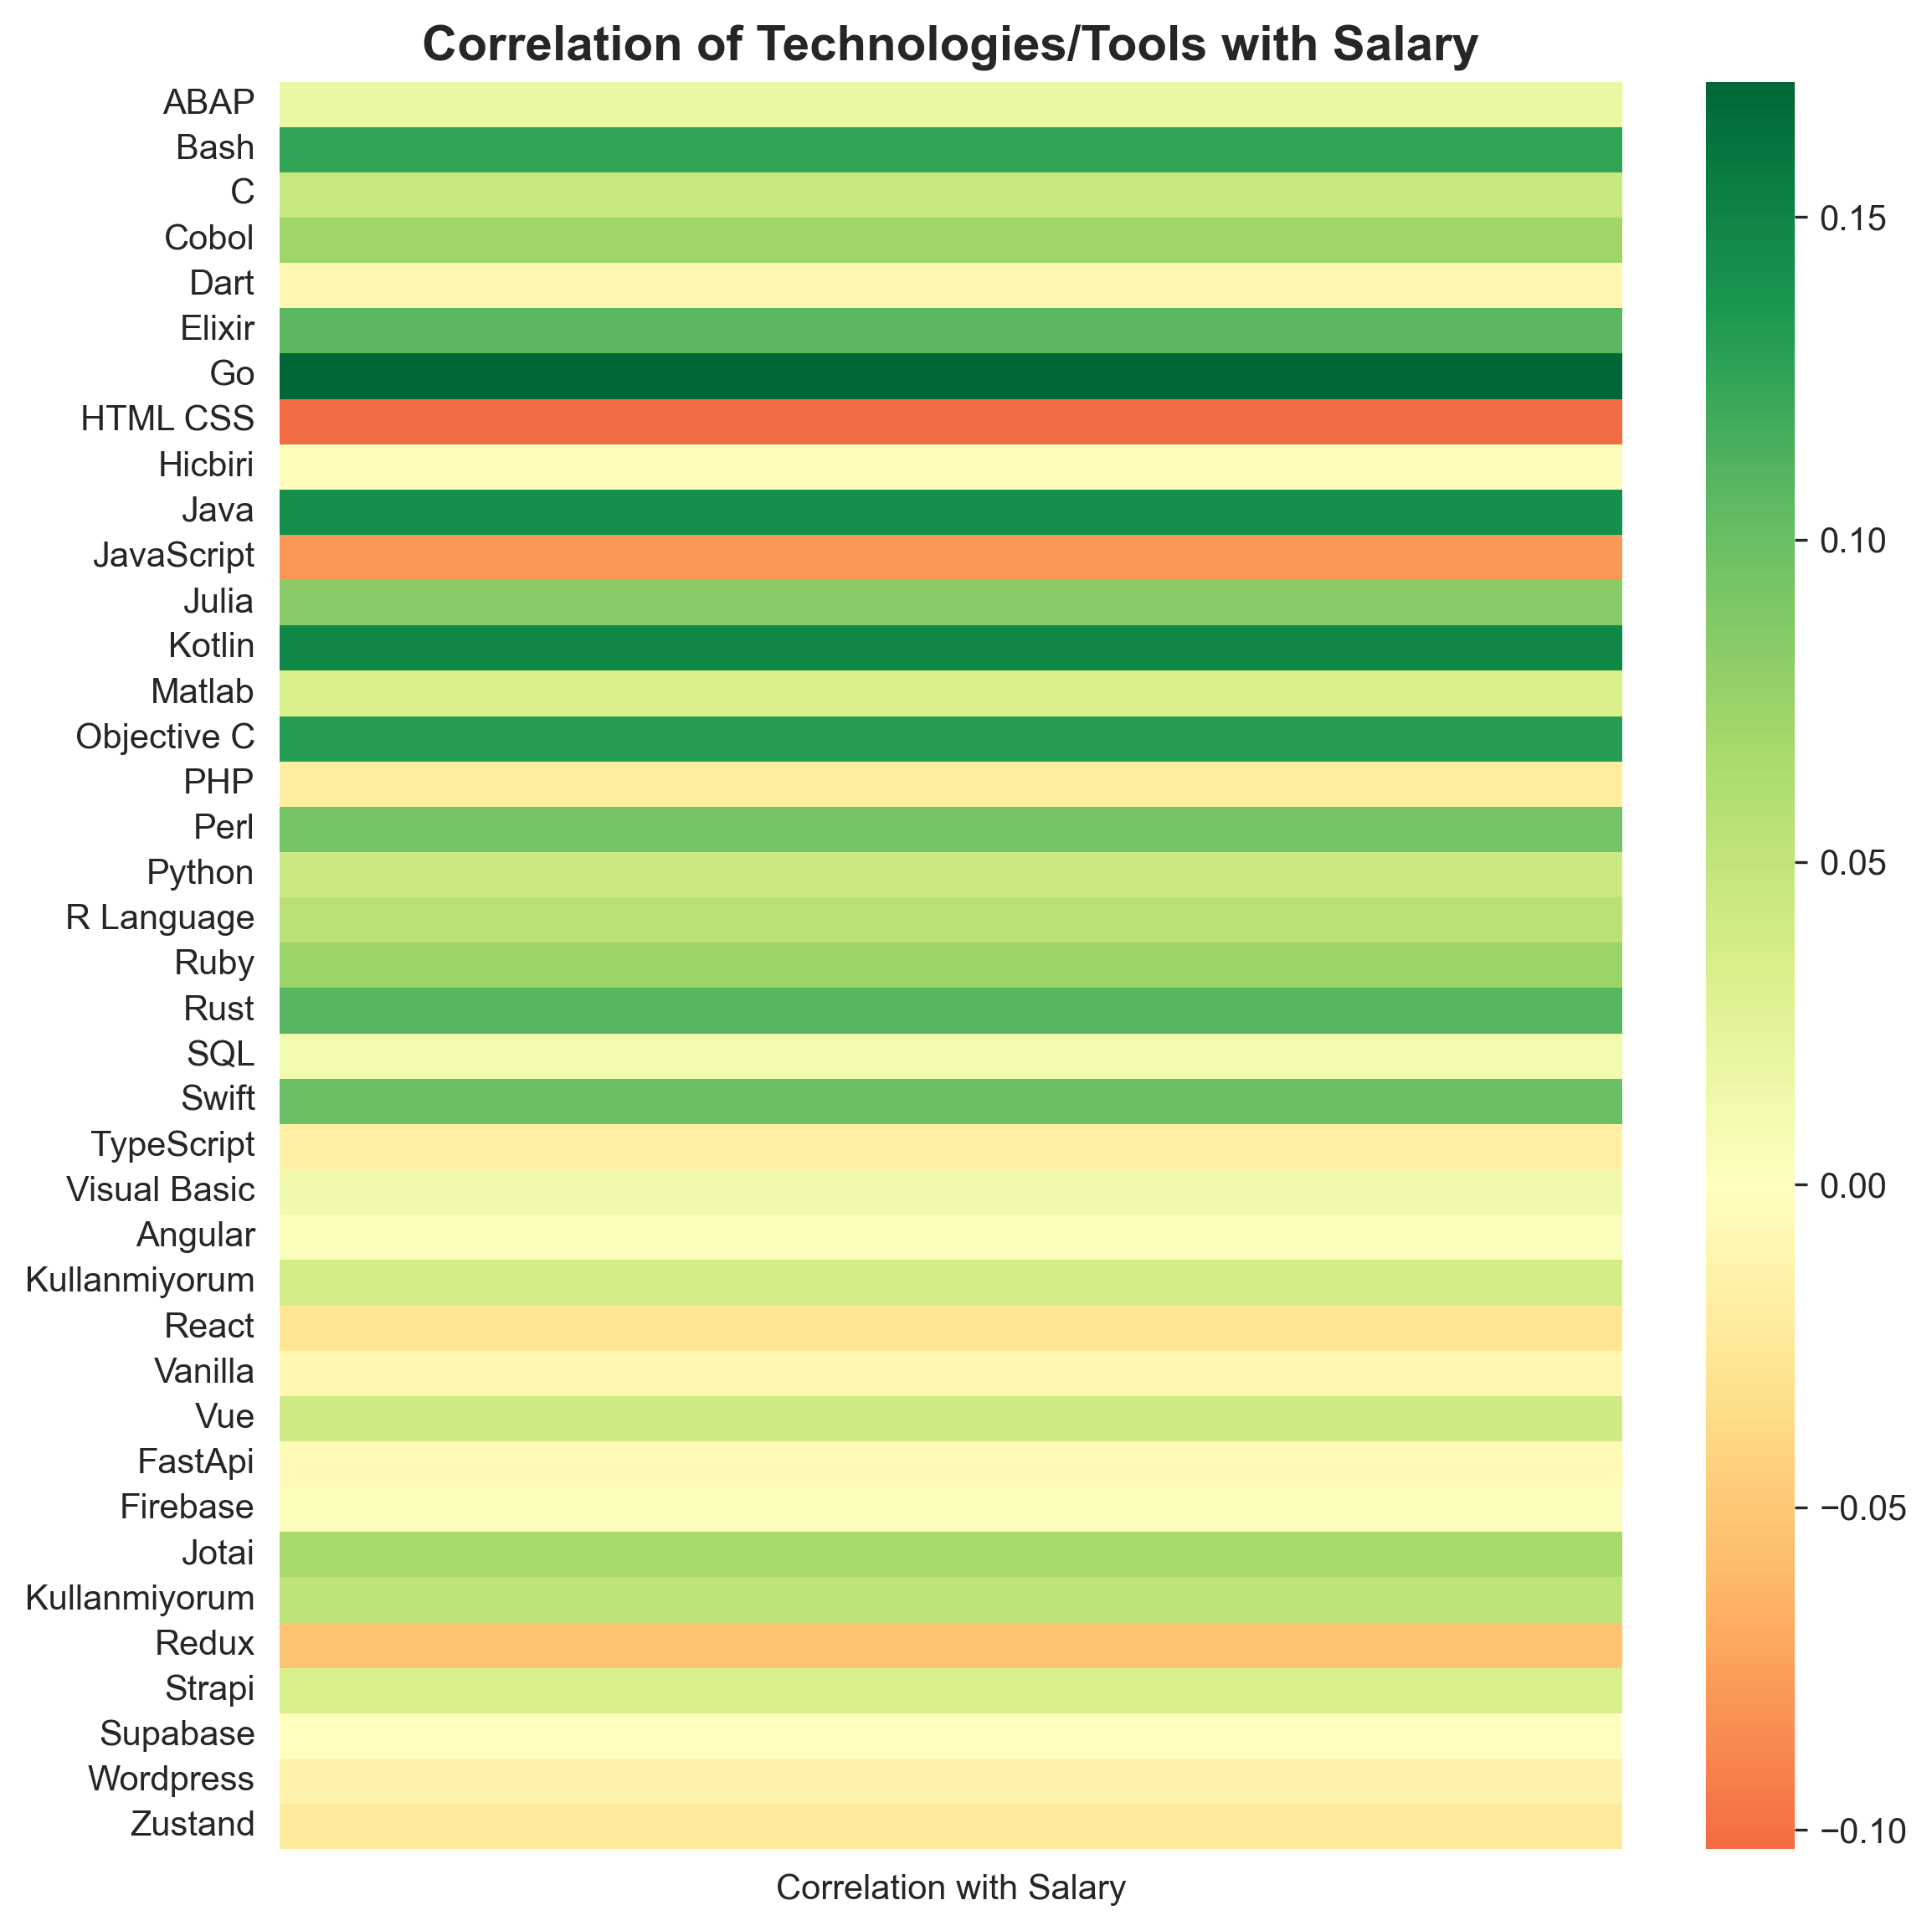
\includegraphics[width=0.8\textwidth]{figures/heatmap_tech_tool_salary.png}
	\caption{Technology-Salary Correlations}
\end{figure}

% Methodological note
\textbf{What is Correlation?}
Correlation is a statistical metric that measures the direction and strength of the linear relationship between two variables. In our report, the \textbf{correlation coefficient (r)} ranges from -1 to +1.

* A \textbf{positive correlation} (close to +1) indicates that professionals using a certain technology tend to have higher salaries.
* A \textbf{negative correlation} (close to -1) suggests the opposite.
* A correlation close to \textbf{zero} means there is no clear linear relationship between the technology and salary.

It is crucial to note that correlation does not imply causation. A strong relationship between a technology and salary may simply indicate that this technology is commonly used in higher-paying roles, rather than being the direct cause of the salary increase.

% Streamlined insights
\textbf{Key Insights:}
\begin{itemize}
    \item \textbf{High-Correlation Technologies}: Go (r = 0.171), Kotlin (r = 0.147), and Rust (r = 0.108) show the strongest positive correlations with salary, reflecting niche demand.
    \item \textbf{Market Demand}: Technologies with r \(\geq 0.1\) (e.g., Go, Kotlin, Java, Objective C) indicate higher market value compared to widely used tools like JavaScript (r = -0.080).
    \item \textbf{Skill Stack Strategy}: Combining high-value technologies (e.g., Rust, Go) with tools like React or Docker may boost salaries by 15-25\%, though data is limited.
\end{itemize}

\section{Survey Participation Patterns: When Do Professionals Respond?}

% Compact hourly participation analysis
\subsection{Hourly Participation}
Survey responses over a 2-day window (August 20-21, 2025) show distinct patterns.

\begin{table}[H]
	\centering
	\small
	\begin{tabular}{lrr}
		\toprule
		\textbf{Time Period} & \textbf{Participants (\%)} & \textbf{Avg Salary (k TL)} \\
		\midrule
		Morning (6-11)       & 114 (4.2)                  & 94.7                       \\
		Afternoon (12-17)    & 2095 (76.7)                & 96.4                       \\
		Evening (18-22)      & 599 (21.9)                 & 101.0                      \\
		Night (23-5)         & 158 (5.8)                  & 103.9                      \\
		\bottomrule
	\end{tabular}
	\caption{Participation and Salary by Time Period}
\end{table}

\begin{figure}[H]
	\centering
	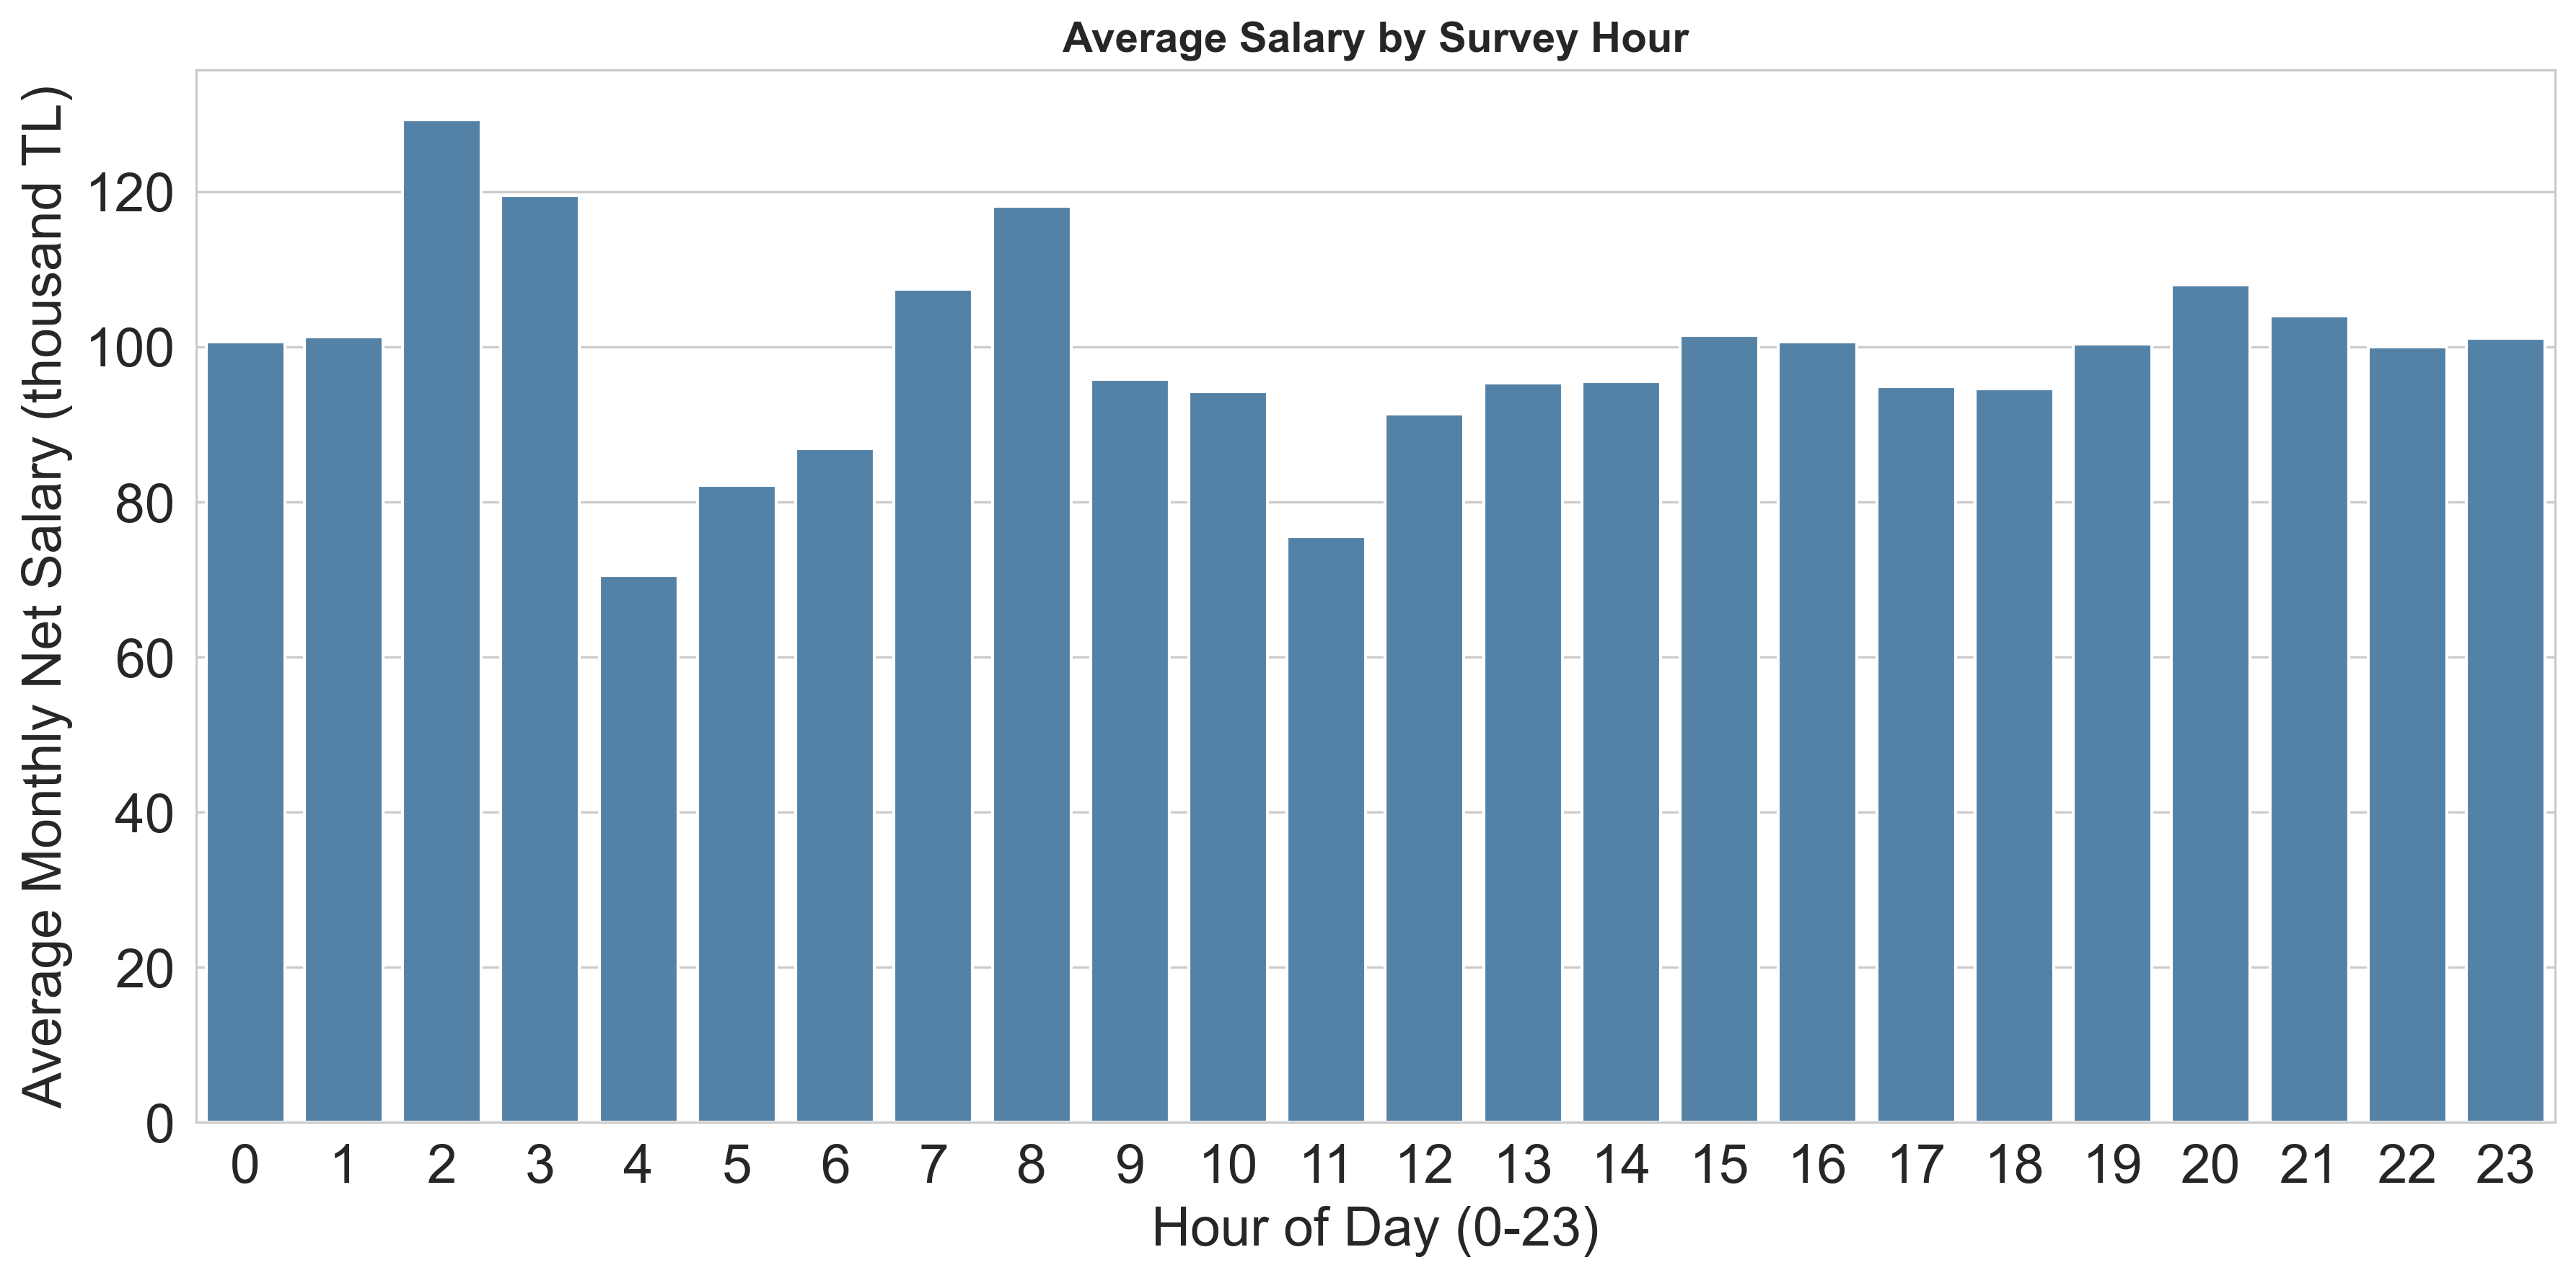
\includegraphics[width=0.8\textwidth]{figures/barplot_hourly_avg_salary.png}
	\caption{Average Salary by Hour}
\end{figure}

\begin{figure}[H]
	\centering
	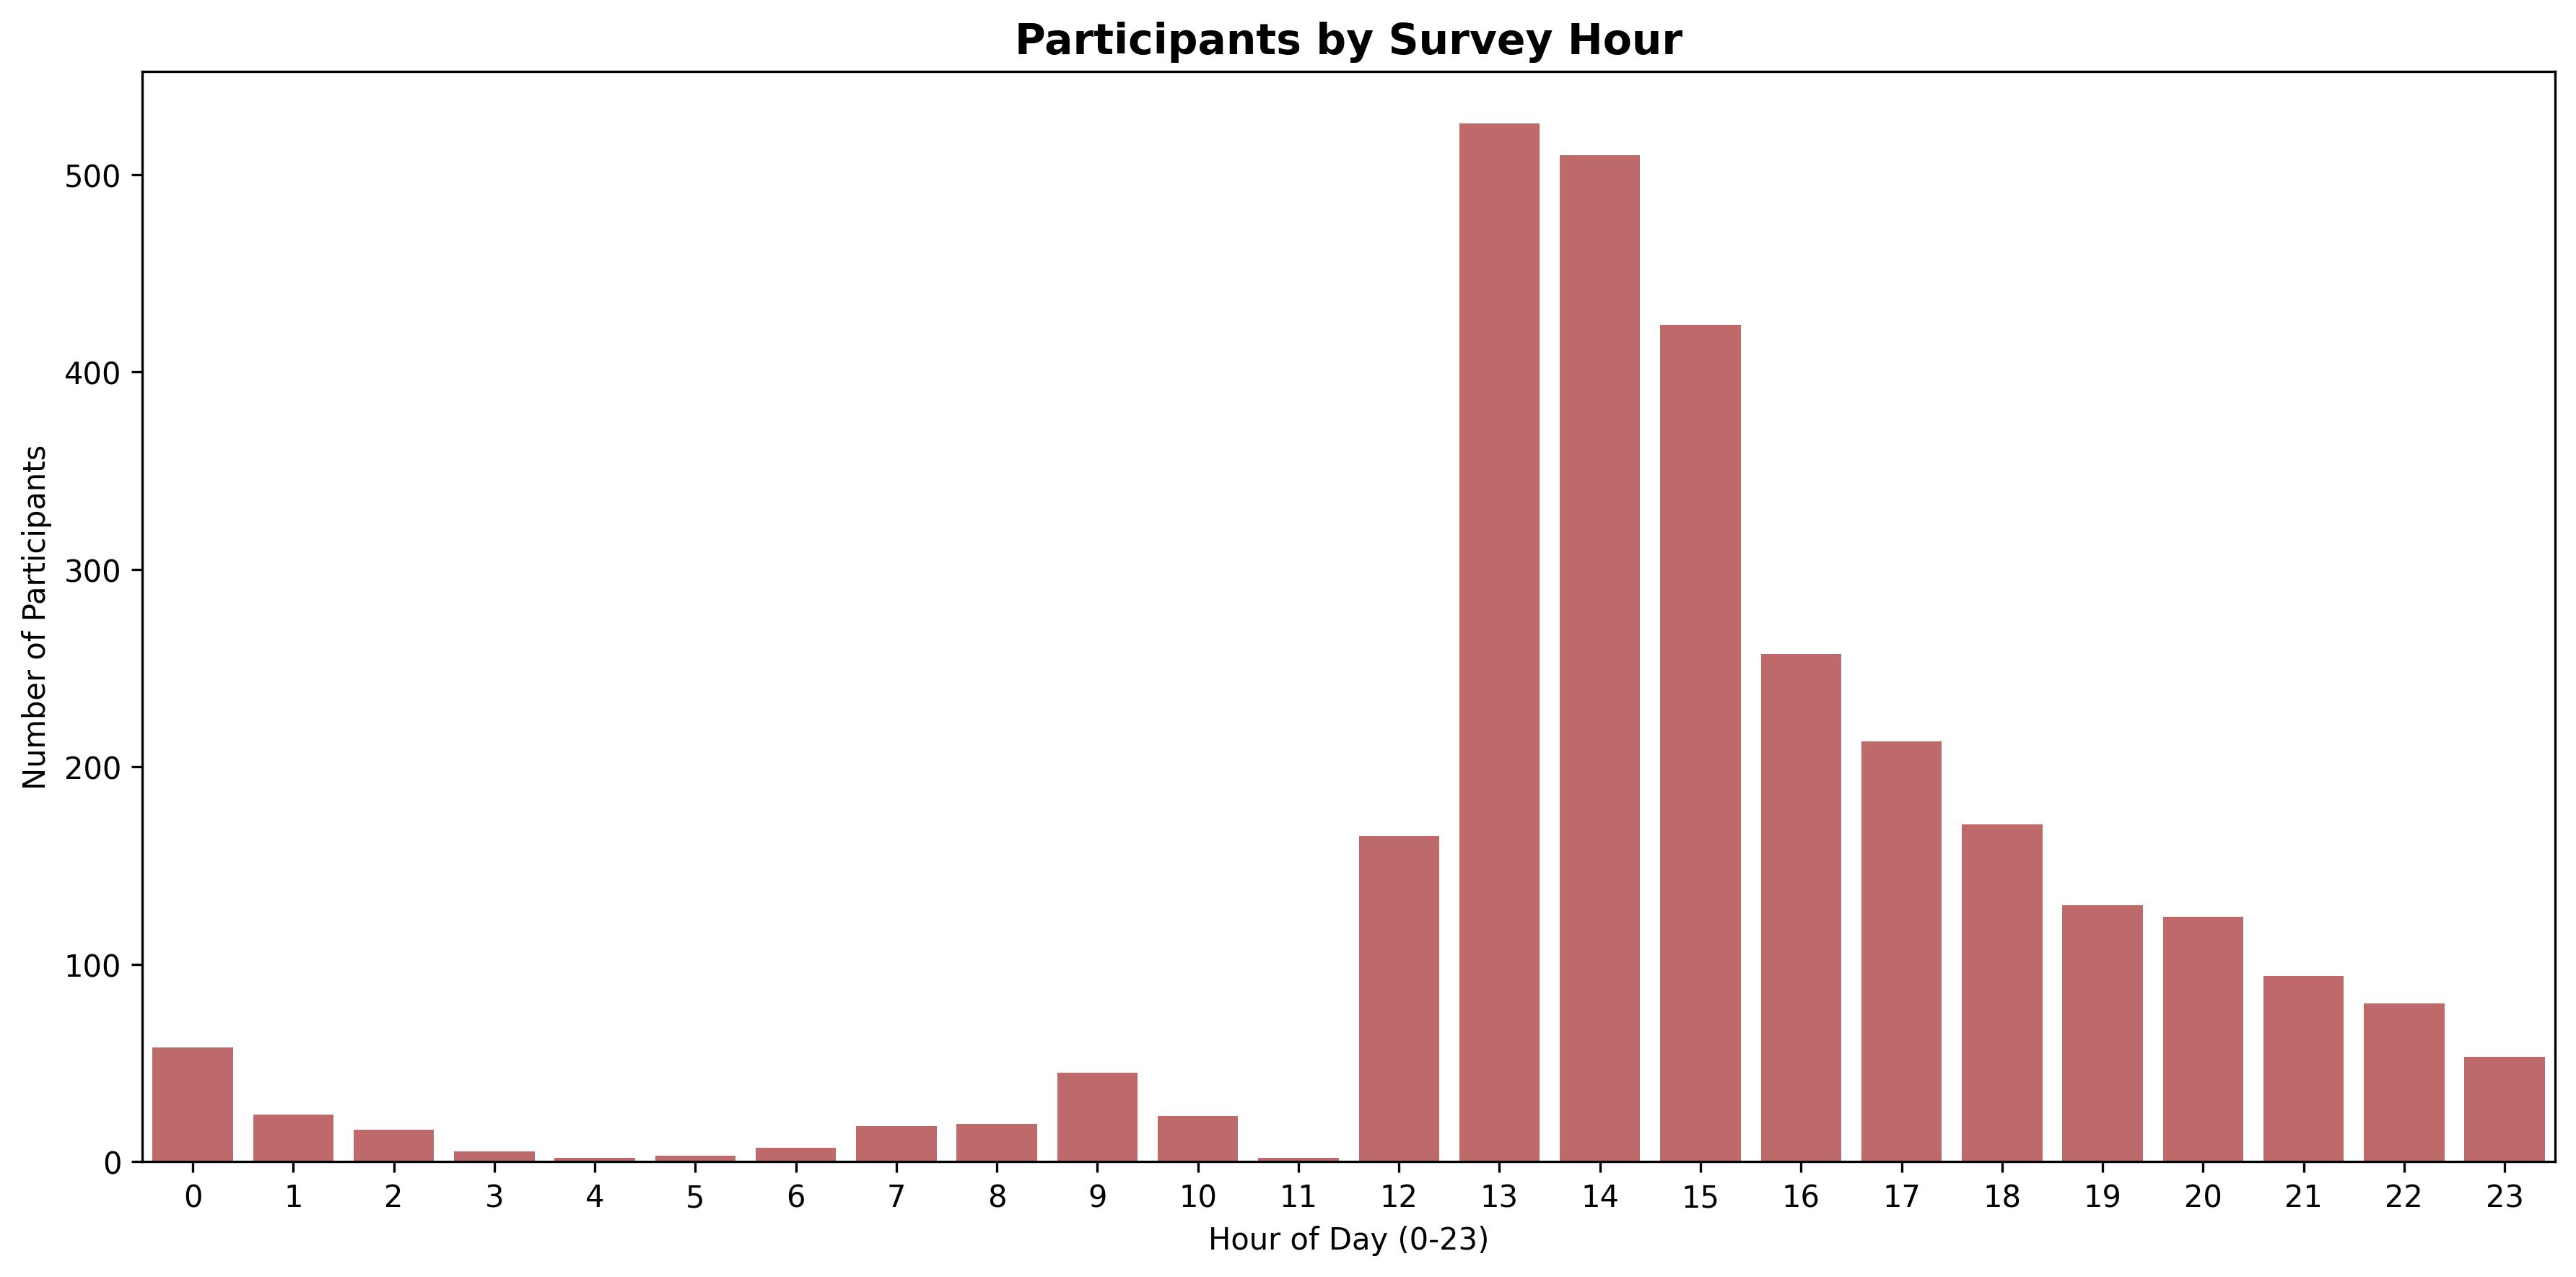
\includegraphics[width=0.8\textwidth]{figures/barplot_hourly_participants.png}
	\caption{Participants by Hour}
\end{figure}

\begin{figure}[H]
	\centering
	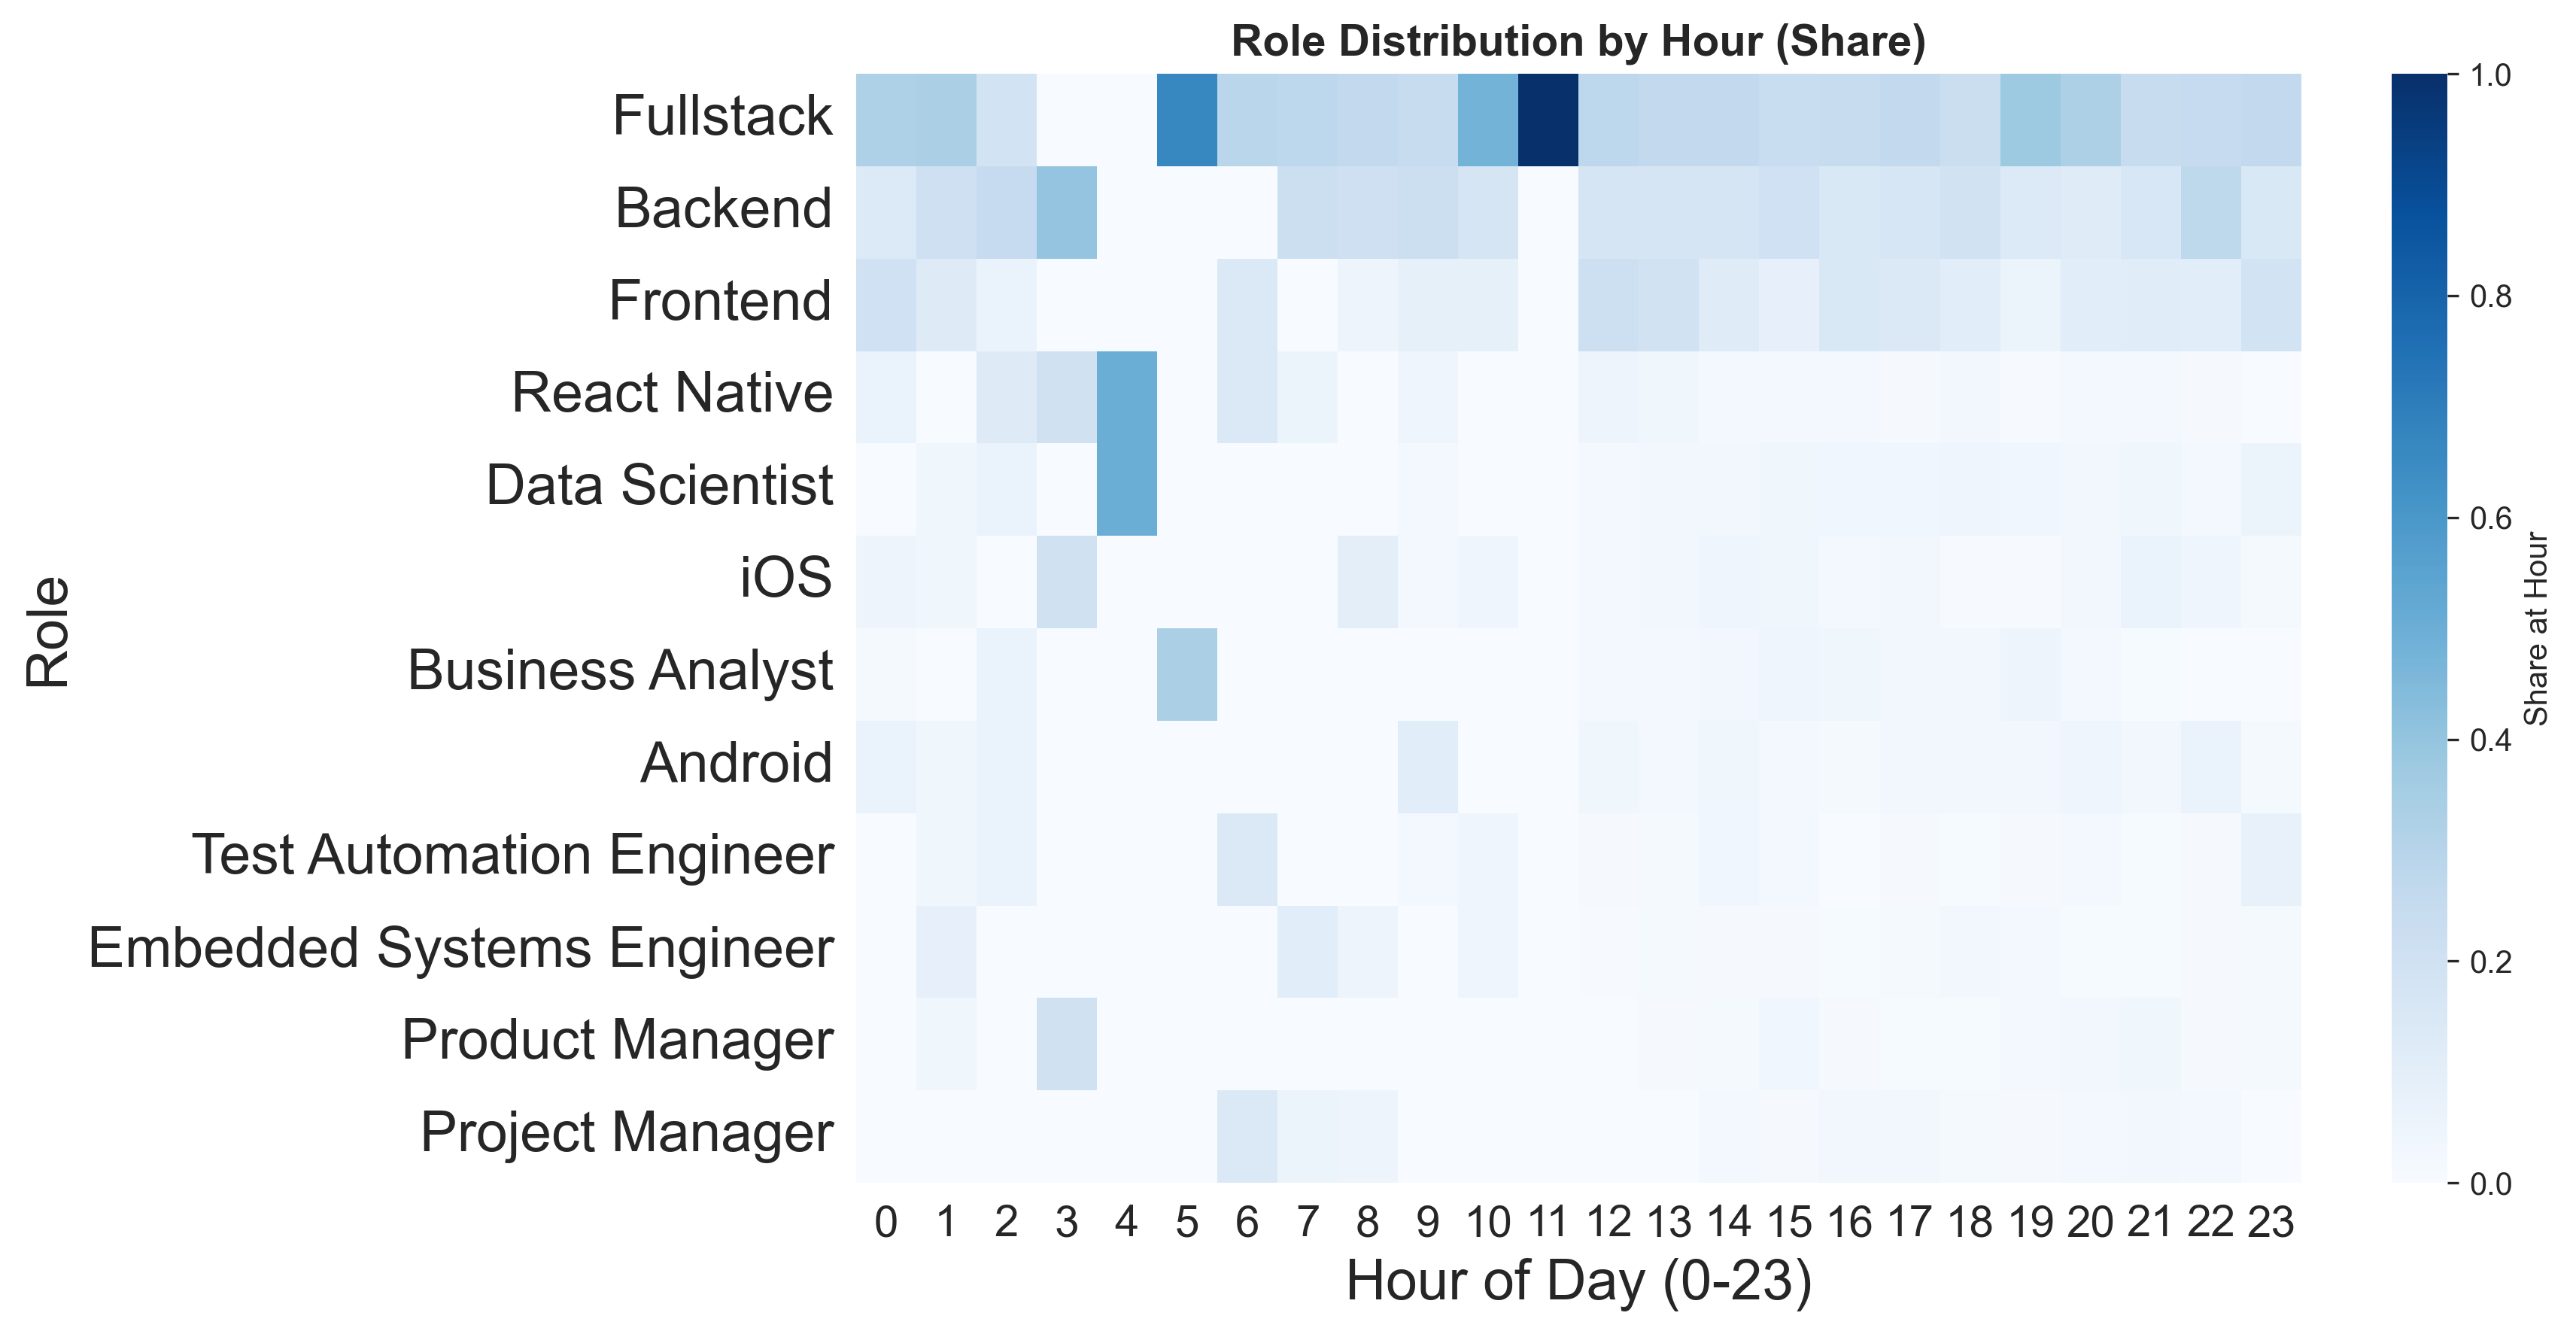
\includegraphics[width=0.8\textwidth]{figures/heatmap_roles_by_hour.png}
	\caption{Role Share by Hour}
\end{figure}

% Methodological considerations
\textbf{Methodological Considerations:}
\begin{itemize}
	\item \textbf{Limited Window}: The 2-day survey (August 20-21, 2025) captures a snapshot, not long-term trends.
	\item \textbf{Response Bias}: The short period may introduce time-of-day biases.
	\item \textbf{Cross-Sectional}: Patterns reflect the 48-hour window and may not generalize.
    \item \textbf{Time Zone Impact}: All temporal data is based on the time zone of the survey's origin (Türkiye, UTC+3). This may affect the observed hourly patterns due to participation from different time zones, such as Europe or America.
\end{itemize}

% Streamlined insights
\textbf{Key Insights:}
\begin{itemize}
	\item \textbf{Response Timing}: Afternoon hours (12-17) dominate with 76.7\% of responses, peaking at 13-15 (53.5\%).
	\item \textbf{Salary Patterns}: Evening (18-22, 101.0 k TL) and night (23-5, 103.9 k TL) respondents earn slightly more than afternoon (96.4 k TL).
	\item \textbf{Role Differences}: Fullstack (30.4\% share) and Backend (16.2\%) are top roles; morning vs. evening preferences are speculative without hourly role data.
    \item \textbf{Survey Validity}: Broad participation across hours supports data reliability within the 2-day window.
\end{itemize}

\section{Career Progression Visualization: The Path Forward}

\subsection{Career Level to Role Flows}
Career progression shows diverse paths from Junior to specialized and management roles.

\begin{figure}[H]
    \centering
    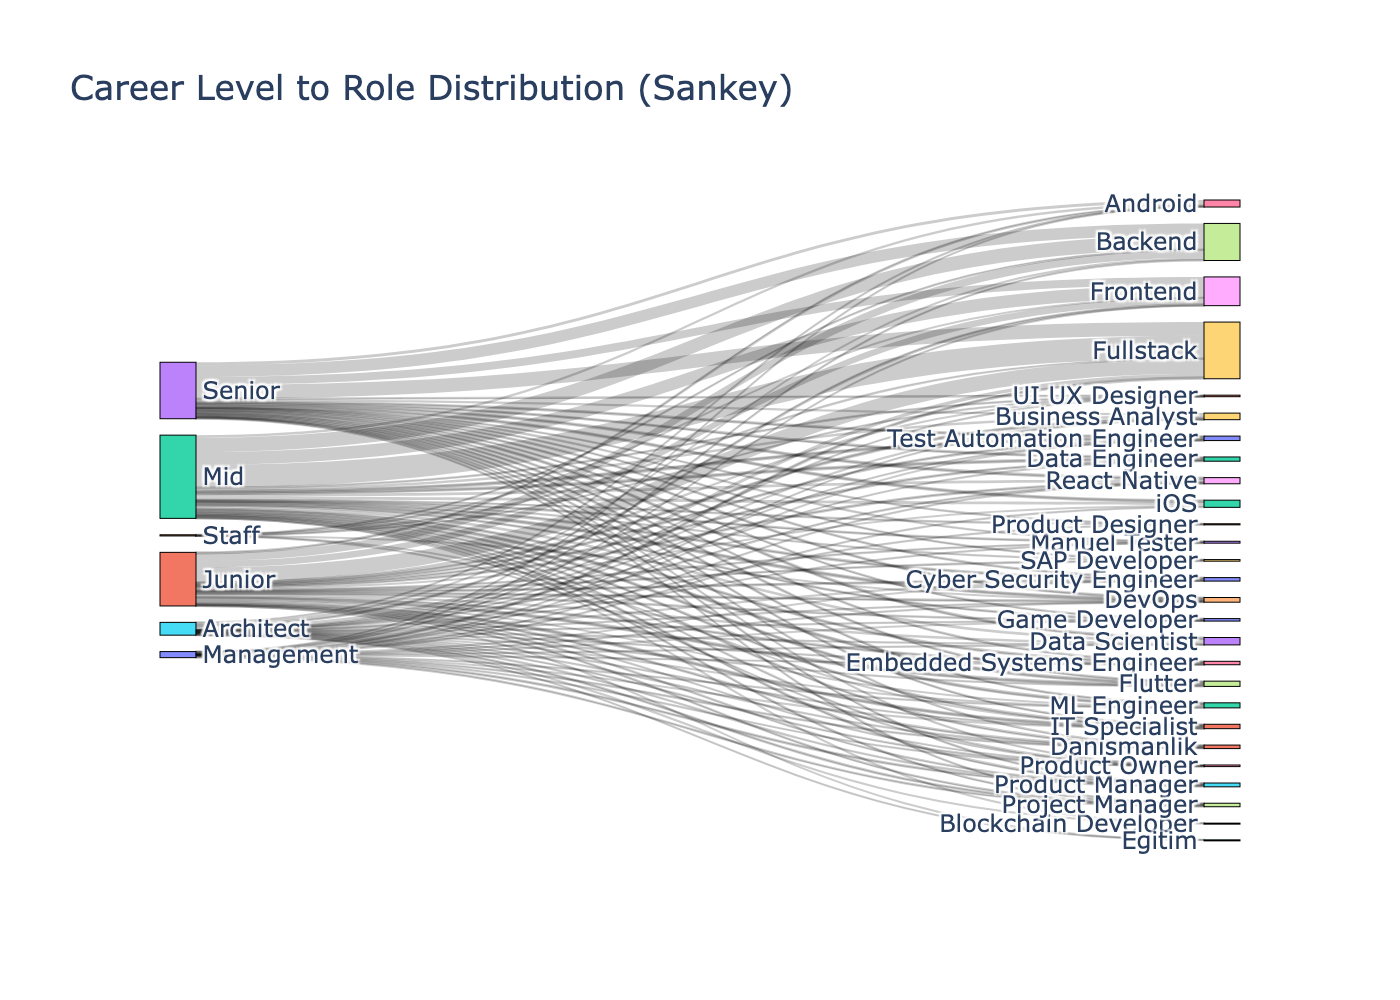
\includegraphics[width=\textwidth]{figures/sankey_career_level_role.png}
    \caption{Career Level to Role Distribution (Sankey) - Professional progression patterns and role transitions}
\end{figure}

\begin{table}[H]
    \centering
    \small
    \begin{tabular}{llr}
        \toprule
        \textbf{Career Level} & \textbf{Role} & \textbf{Count} \\
        \midrule
        Mid                   & Fullstack     & 310            \\
        Junior                & Fullstack     & 204            \\
        Mid                   & Backend       & 198            \\
        Senior                & Fullstack     & 187            \\
        Mid                   & Frontend      & 173            \\
        Senior                & Backend       & 160            \\
        Senior                & Frontend      & 111            \\
        Junior                & Backend       & 105            \\
        Junior                & Frontend      & 89             \\
        Team Lead             & Fullstack     & 46             \\
        \bottomrule
    \end{tabular}
    \caption{Top 10 Career Level to Role Flows}
\end{table}

\textbf{For a detailed and interactive exploration of these career paths, visit our Streamlit dashboard:} \href{http://maas-anketi.streamlit.app/#career-level-role-flow-sankey}{\texttt{maas-anketi.streamlit.app}}

\textbf{Methodological Note:} Counts represent the number of respondents in each career level-role combination:
\[
    \text{Count} = \sum_{i \in \text{Level, Role}} \text{Respondent}_i
\]
Data reflects the most frequent transitions from a survey of professionals.

\textbf{Key Insights:}
\begin{itemize}
    \item \textbf{Role Transitions}: Fullstack roles are a common path across all levels (Mid: 310, Junior: 204, Senior: 187), showing significant flows from junior to senior levels.
    \item \textbf{Career Paths}: In addition to Fullstack, Backend (Mid: 198, Senior: 160) and Frontend (Mid: 173, Senior: 111) are also highly prevalent career paths.
    \item \textbf{Specialization Premium}: Specialized roles like Staff Engineer and Architect are associated with significantly higher salaries, commanding premiums of 44-48\% over Senior roles.
    \item \textbf{Management Premium}: Management roles, such as Engineering Manager, yield substantial salary increases (37-41\%) over Senior-level positions.
\end{itemize}

\section{Employment Type Analysis: Full-time vs Freelance}

% Compact employment type salary comparison
\subsection{Employment Type Salaries}
Employment types show distinct salary patterns, reflecting stability and flexibility trade-offs.

\begin{table}[H]
	\centering
	\small
	\begin{tabular}{lrrr}
		\toprule
		\textbf{Employment Type} & \textbf{Count} & \textbf{Mean Salary (k TL)} & \textbf{\% Diff. vs Full-time} \\
		\midrule
		Self-employed            & 40             & 123.4                       & 24.6                           \\
		Full-time                & 2837           & 99.0                        & --                             \\
		Freelance                & 36             & 94.4                        & -4.6                           \\
		Part-time                & 56             & 43.0                        & -56.6                          \\
		\bottomrule
	\end{tabular}
	\caption{Salary by Employment Type}
\end{table}

\begin{figure}[H]
	\centering
	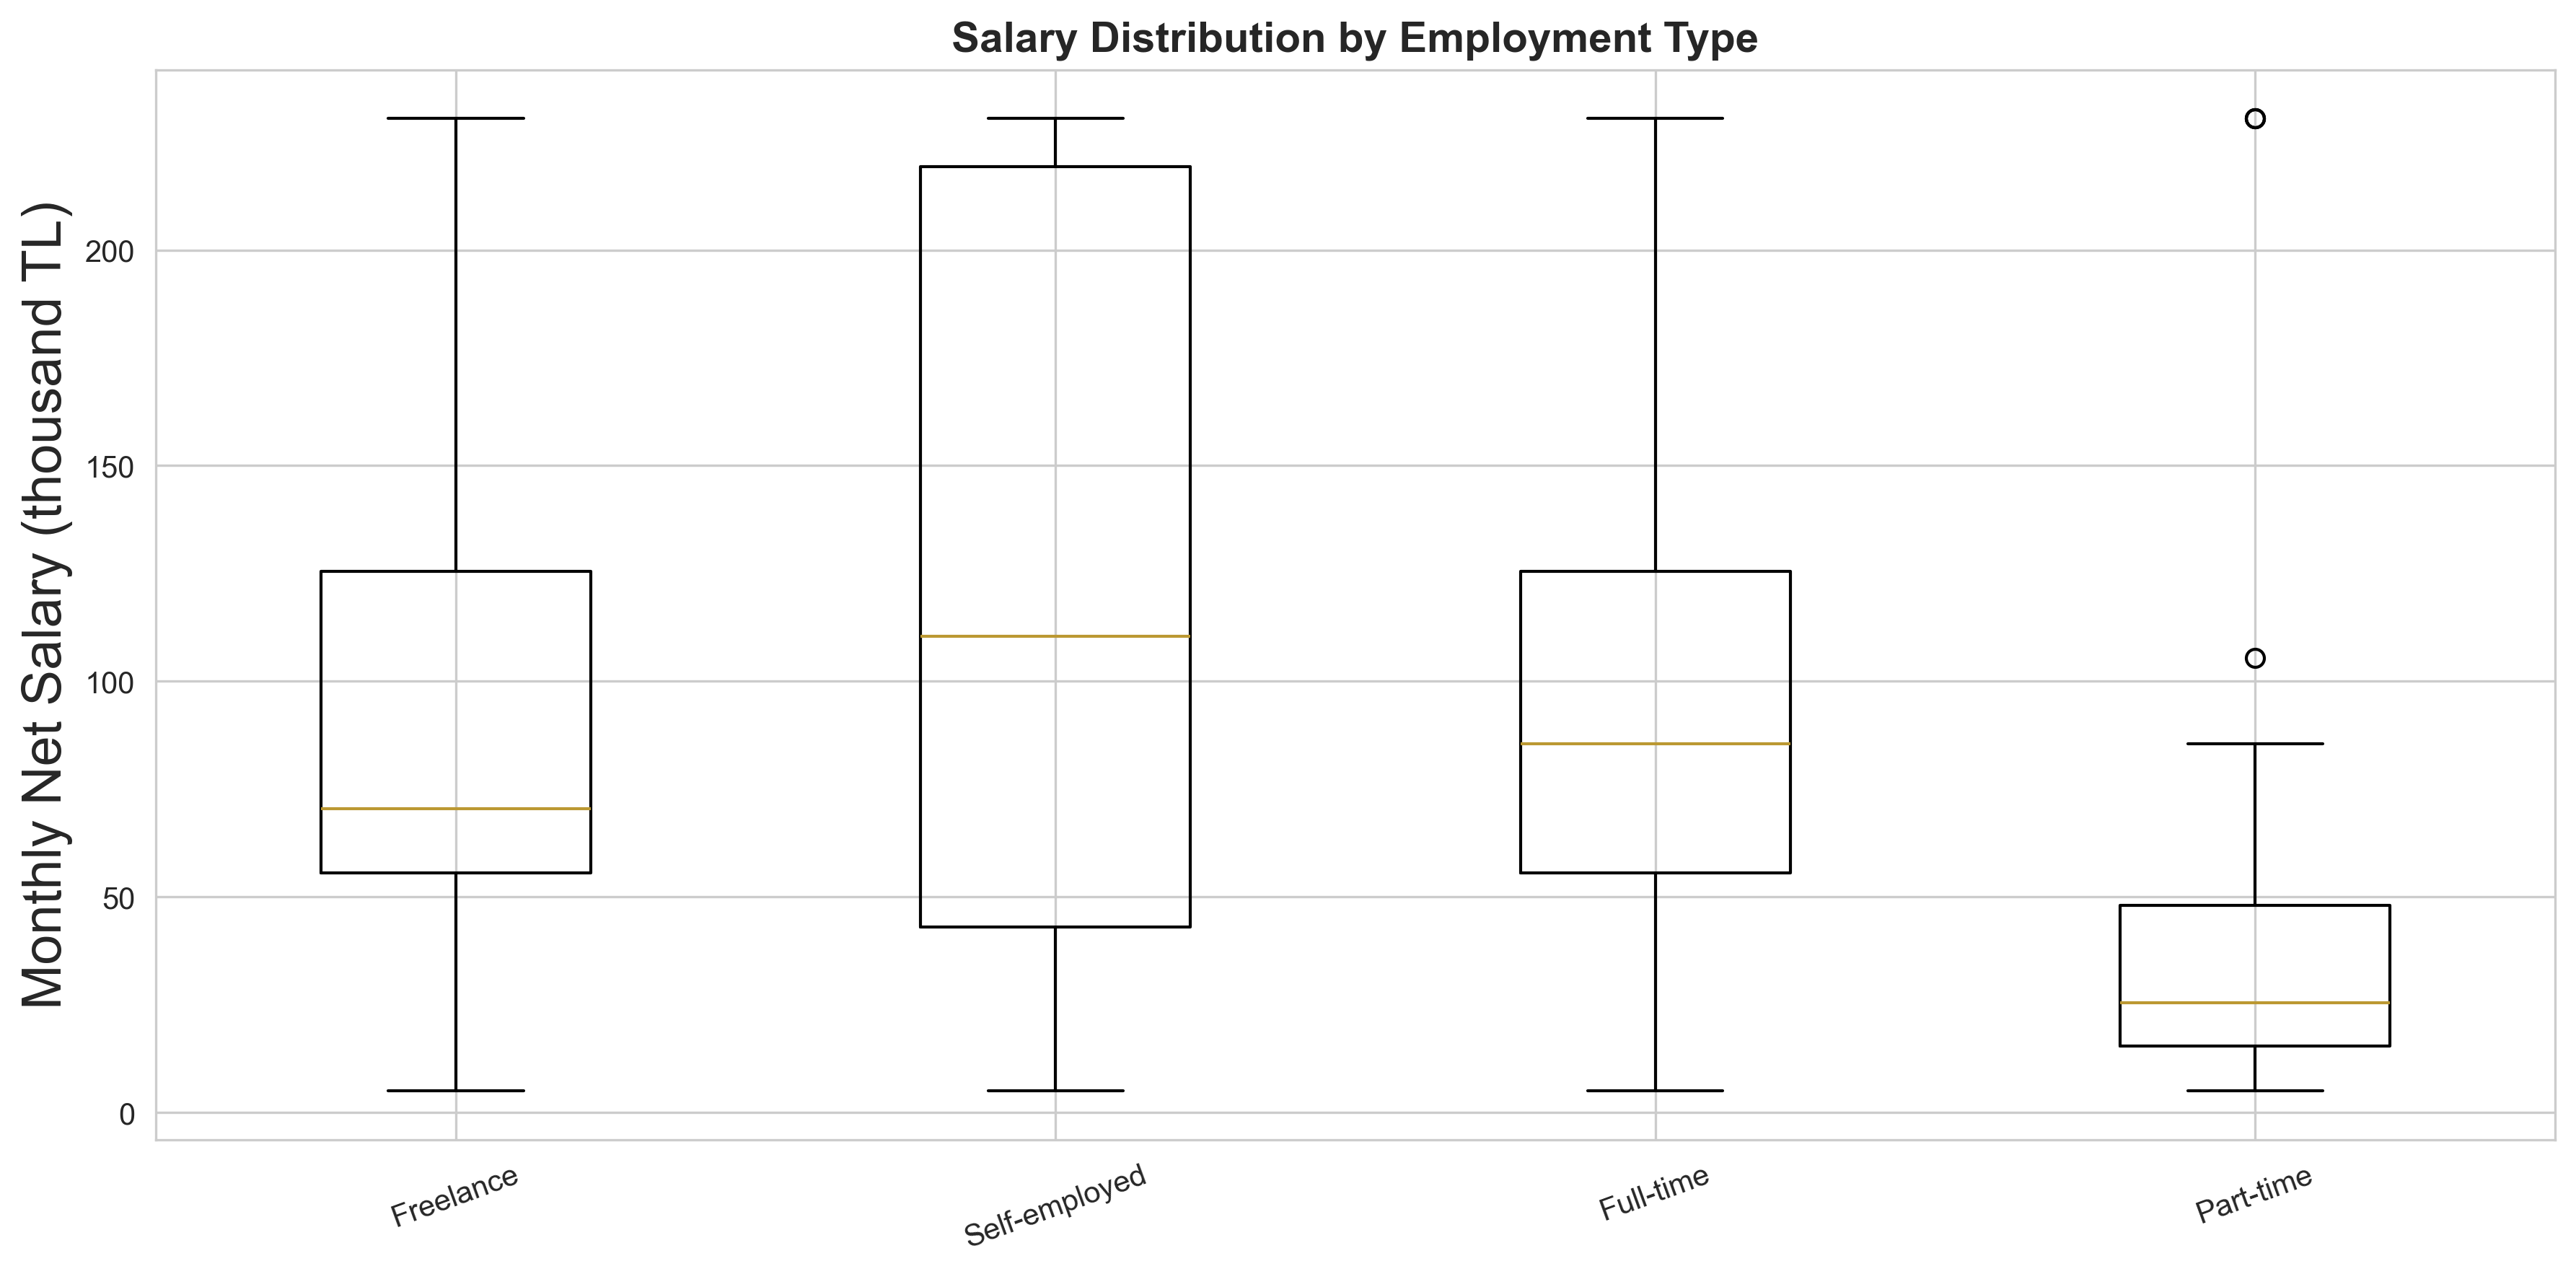
\includegraphics[width=0.8\textwidth]{figures/boxplot_employment_type.png}
	\caption{Salary by Employment Type}
\end{figure}

% Methodological note
\textbf{Methodological Note:}
Mean salary is calculated as:
\[
	\text{Mean Salary} = \frac{\sum_{i \in \text{Group}} \text{Salary}_i}{n}
\]
Percentage difference is:
\[
	\text{\% Diff.} = \left( \frac{\text{Mean}_{\text{Type}} - \text{Mean}_{\text{Full-time}}}{\text{Mean}_{\text{Full-time}}} \right) \times 100
\]
Salaries reflect annual earnings; hourly rates are not available.

% Streamlined insights
\textbf{Key Insights:}
\begin{itemize}
	\item \textbf{Full-time Premium}: Full-time employees (99.0 k TL) earn 130.2\% more than Part-time (43.0 k TL), with stability and benefits.
	\item \textbf{Freelance Flexibility}: Freelance (94.4 k TL) earns 4.6\% less annually than Full-time, but may have higher hourly rates, with income variability.
	\item \textbf{Part-time Trade-off}: Part-time roles offer flexibility but pay 56.6\% less than Full-time, reflecting reduced hours.
	\item \textbf{Self-employed Potential}: Self-employed professionals (123.4 k TL) earn 24.6\% more than Full-time, with higher risk.
\end{itemize}

\section{Advanced Visualizations}

\subsection{Career Progression - Salary Growth}
This line chart shows how salaries evolve from Junior to Senior levels across different company locations. The analysis filters for respondents who are likely in the company location, as per the methodology.

\begin{figure}[H]
	\centering
	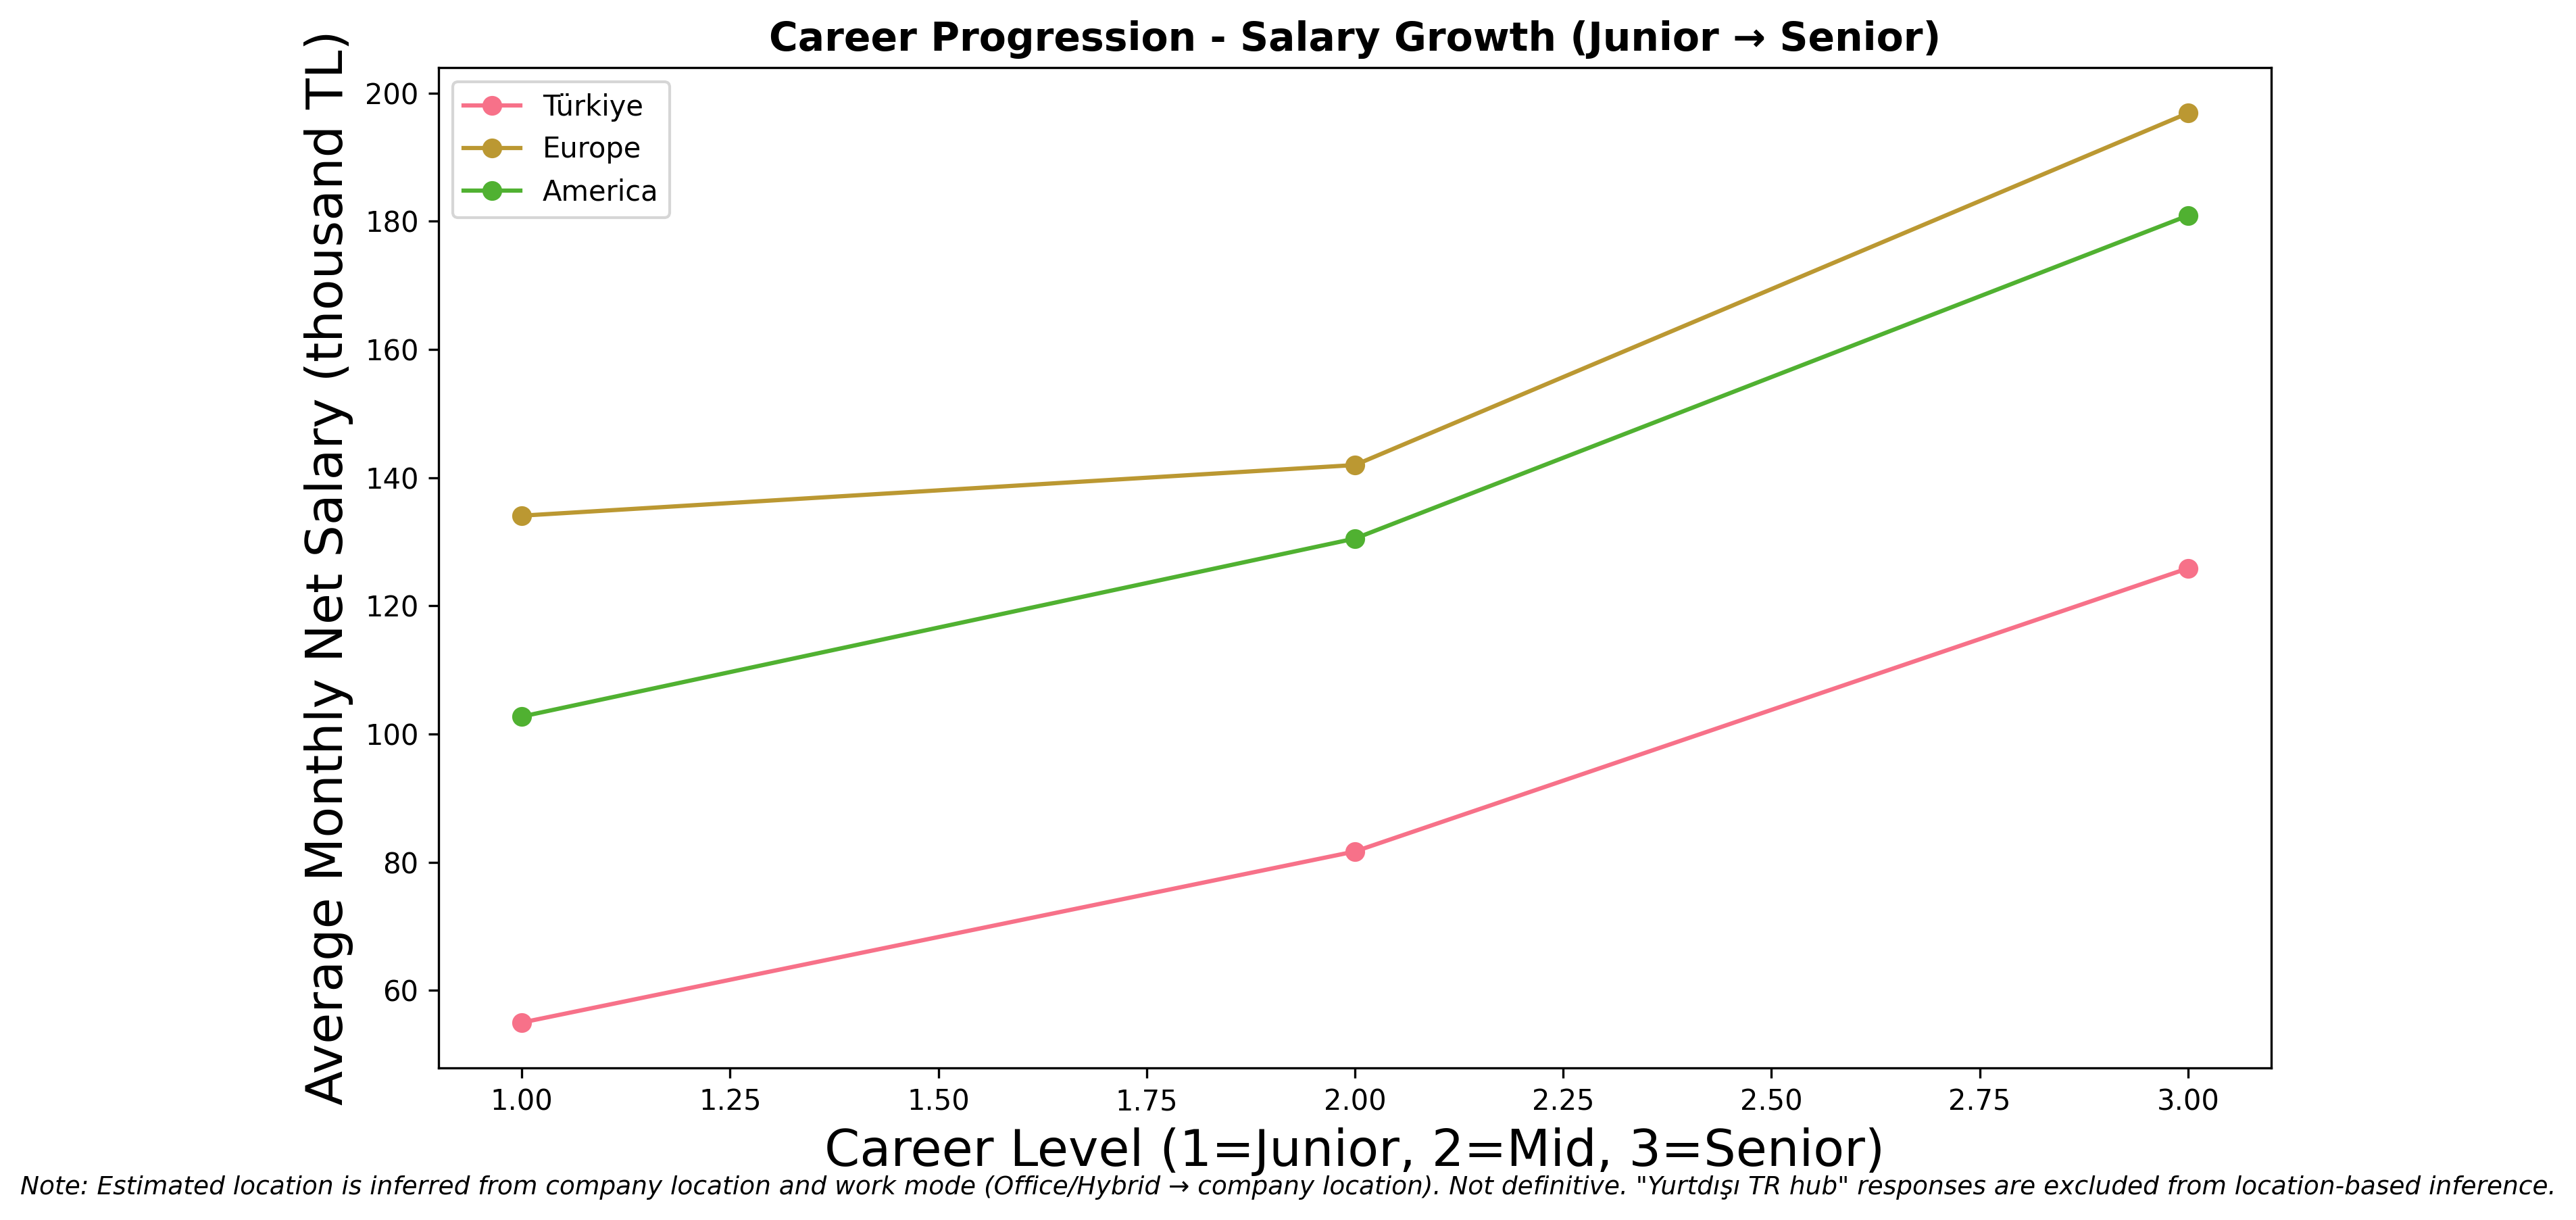
\includegraphics[width=\textwidth]{figures/line_career_progression_salary_growth.png}
	\caption{Career Progression - Salary Growth (Junior \textrightarrow{} Senior)}
\end{figure}

\textbf{Methodological Note:} Since the survey did not collect data on the respondent's residency, all location-based analyses are based on an estimated location. The assumption is that professionals with a company in a given location (e.g., Europe, America) and a work mode of 'Office' or 'Hybrid' are likely to be physically located in that country. The analysis on this graph is based on this estimated residency.

\begin{table}[H]
	\centering
	\small
	\begin{tabular}{lrrr}
		\toprule
		\textbf{Location} & \textbf{Junior} & \textbf{Mid} & \textbf{Senior} \\
		\midrule
		Türkiye          & 52.4            & 80.6         & 124.6           \\
		Europe            & 112.2           & 130.7        & 194.3           \\
		America           & 102.7           & 130.5        & 180.9           \\
		\bottomrule
	\end{tabular}
	\caption{Average Salary by Career Level and Location (k TL)}
\end{table}

\textbf{Career Progression Insights:}
\begin{itemize}
	\item \textbf{Geographical Salary Premium}: European and American companies offer significantly higher salaries at every career level compared to their Turkish counterparts. A Junior developer in Europe earns more than double that of a Junior in Türkiye (112.2k TL vs. 52.4k TL).
	\item \textbf{Career Growth Trajectory}: The total salary growth from Junior to Senior in Türkiye is 137\%, which is a faster rate than in Europe (121\%) and America (118\%). This indicates that while foreign companies offer a higher salary floor and ceiling, the growth trajectory within Türkiye is proportionally steeper.
\end{itemize}

\subsection{Top Tech Combinations by Role}
This bar chart shows the average salaries for prominent technology stack combinations (Programming Language + Front-End Technology + Tool), grouped by role. Only combinations with at least 10 respondents are included.

\begin{figure}[H]
	\centering
	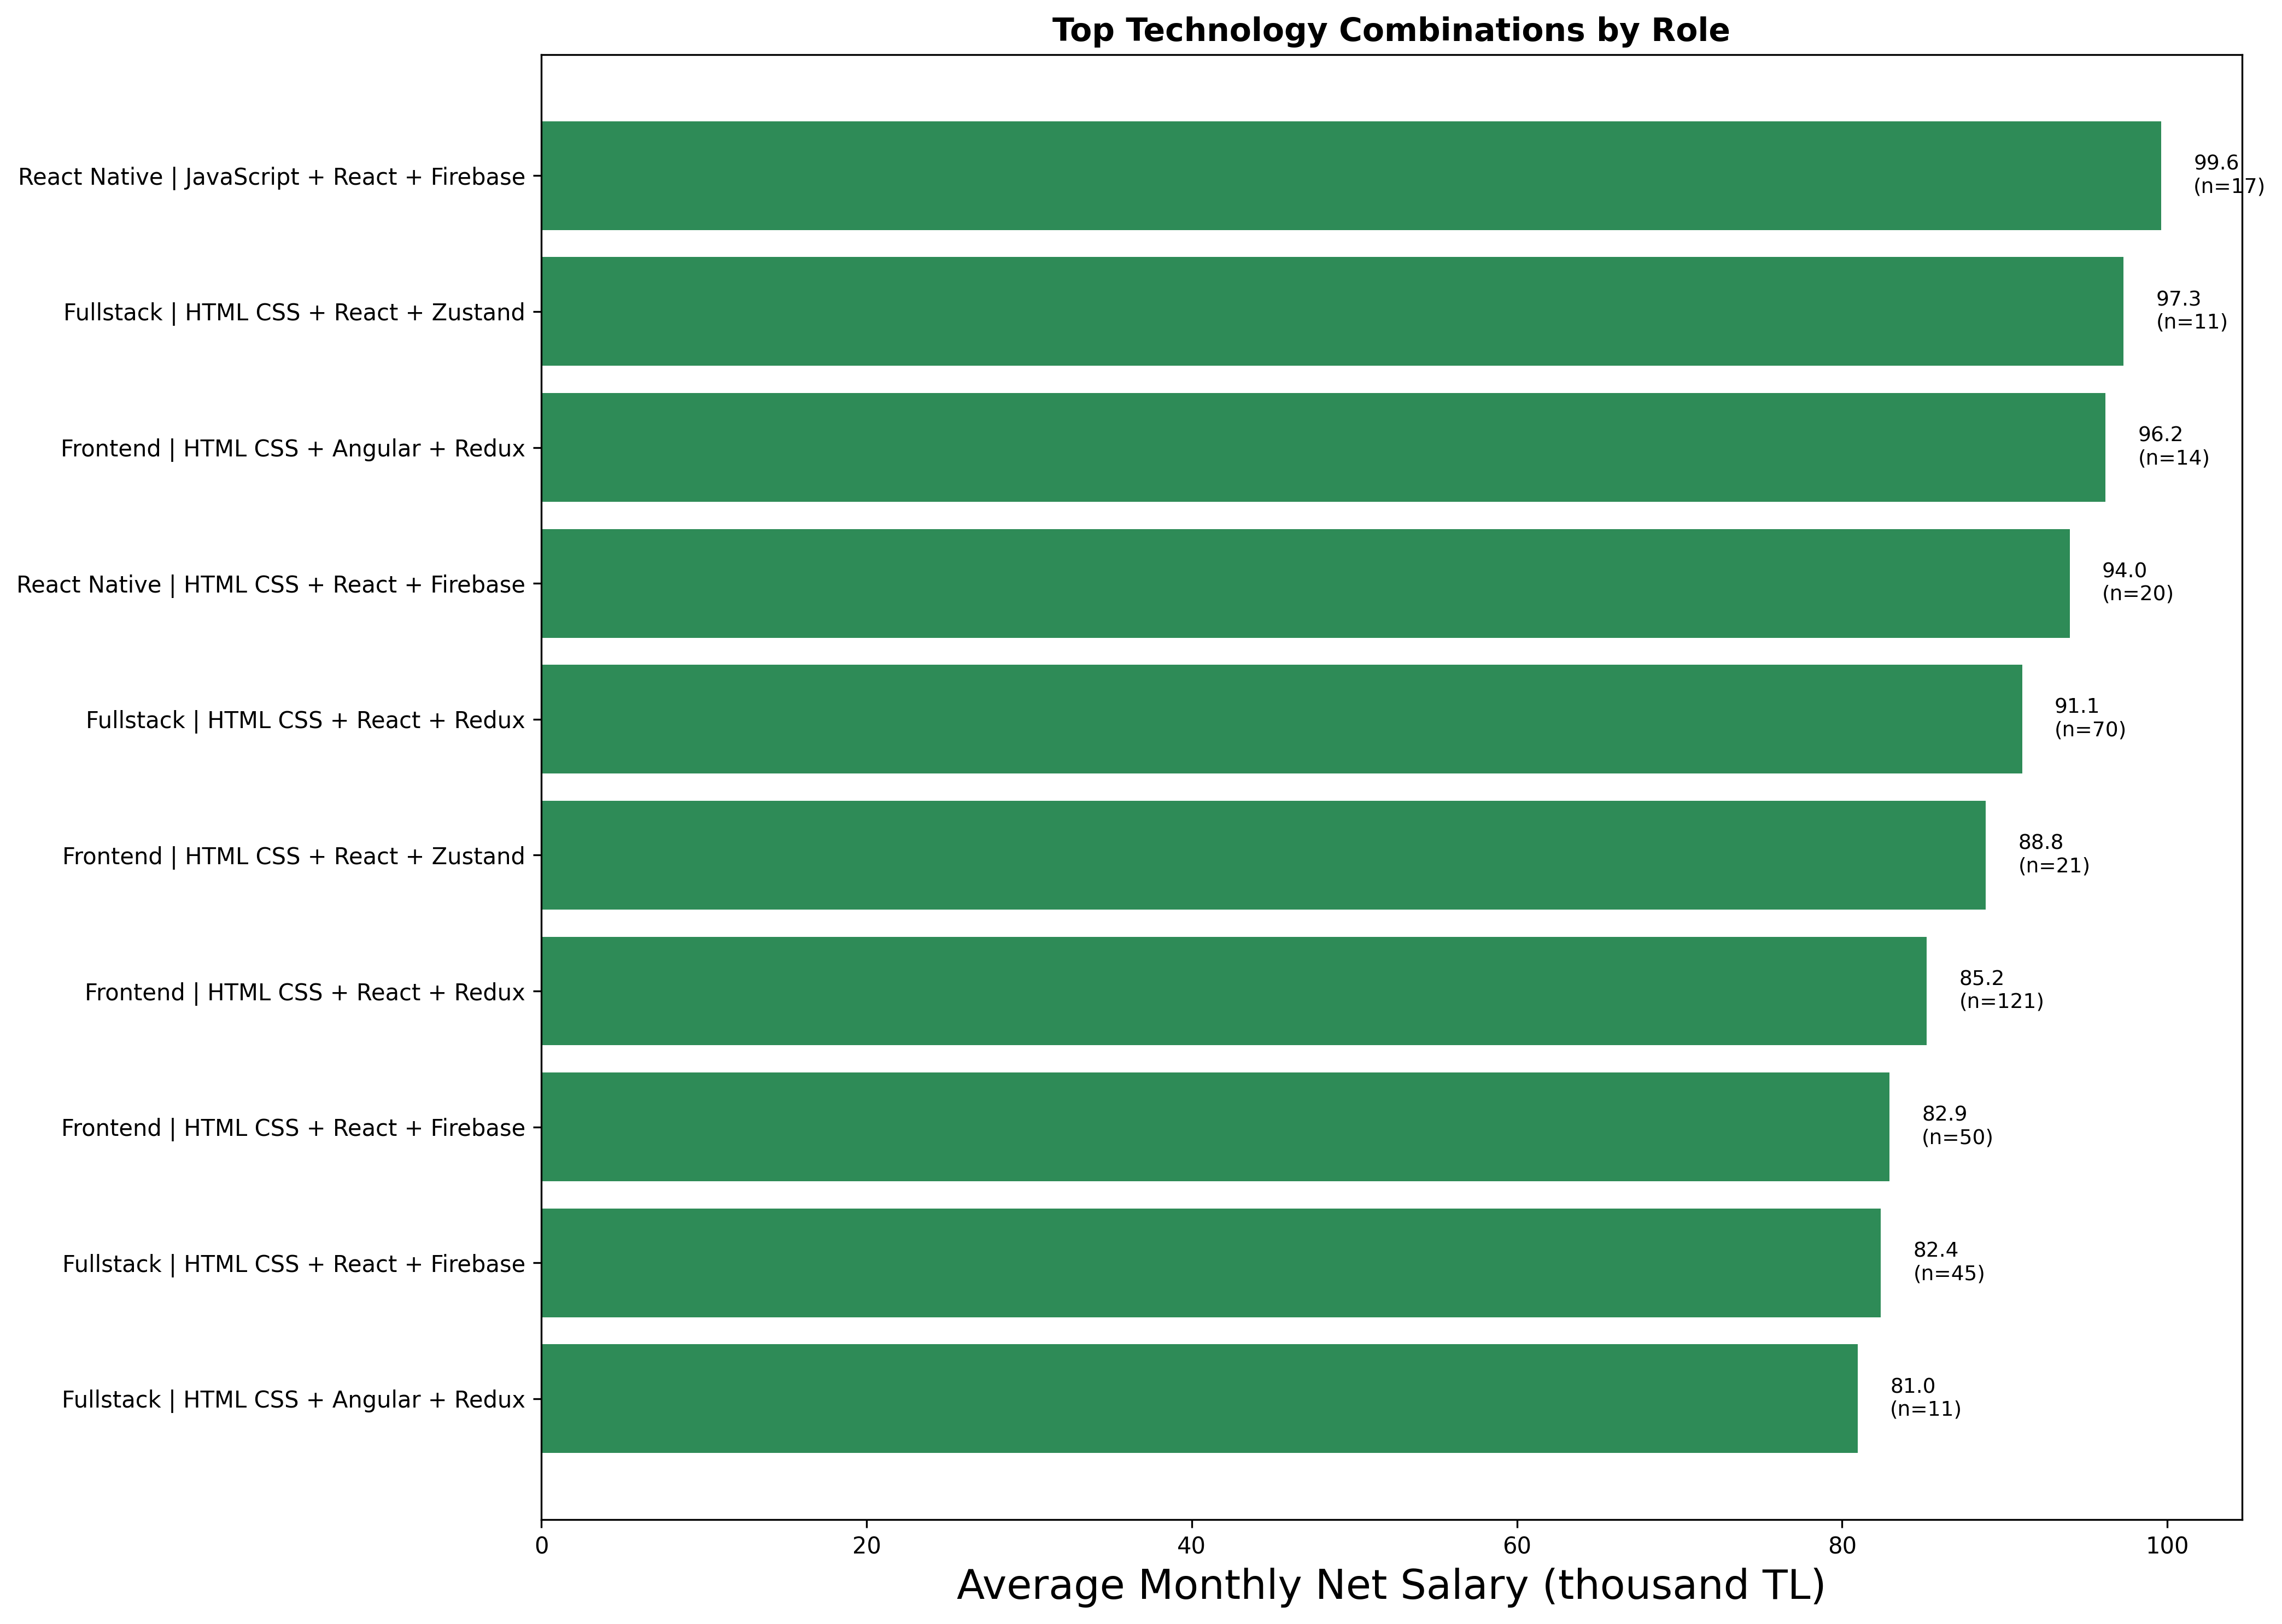
\includegraphics[width=\textwidth]{figures/barplot_tech_combinations_by_role.png}
	\caption{Top Tech Combinations by Role - Average salary for language + frontend + tool stacks (n$\geq$10 per combo)}
\end{figure}

\begin{table}[H]
	\centering
	\small
	\begin{tabular}{llr}
		\toprule
		\textbf{Role | Tech Stack}                   & \textbf{Average Salary} & \textbf{Count} \\
		\midrule
		React Native | JavaScript + React + Firebase & 99.6                    & 17             \\
		Fullstack | HTML CSS + React + Zustand       & 97.3                    & 11             \\
		Frontend | HTML CSS + Angular + Redux        & 96.2                    & 14             \\
		React Native | HTML CSS + React + Firebase   & 94.0                    & 20             \\
		Fullstack | HTML CSS + React + Redux         & 91.1                    & 70             \\
		Frontend | HTML CSS + React + Zustand        & 88.8                    & 21             \\
		Frontend | HTML CSS + React + Redux          & 85.2                    & 121            \\
		Frontend | HTML CSS + React + Firebase       & 82.9                    & 50             \\
		Fullstack | HTML CSS + React + Firebase      & 82.4                    & 45             \\
		Fullstack | HTML CSS + Angular + Redux       & 81.0                    & 11             \\
		Fullstack | HTML CSS + Angular + Firebase    & 78.3                    & 18             \\
		Fullstack | HTML CSS + React + FastApi       & 71.6                    & 34             \\
		Fullstack | JavaScript + React + Redux       & 71.5                    & 15             \\
		Frontend | HTML CSS + React + FastApi        & 68.2                    & 26             \\
		\bottomrule
	\end{tabular}
	\caption{Top Technology Stack Combinations by Average Salary (k TL)}
\end{table}

\textbf{Top Technology Stack Insights:}
\begin{itemize}
	\item \textbf{Highest-Paying Combination}: The top-earning combination is `JavaScript + React + Firebase` within the \textbf{React Native} role, with an average salary of 99.6k TL. This highlights the high demand for a full-stack mobile development skillset.
	\item \textbf{Frontend vs. Fullstack}: The `HTML/CSS + React + Redux` stack shows a notable salary premium for \textbf{Fullstack} developers (91.1k TL) compared to \textbf{Frontend} developers (85.2k TL). This suggests that additional backend skills provide a measurable salary advantage.
	\item \textbf{React Ecosystem}: The data confirms the dominance of React and its ecosystem, with all top 14 combinations featuring either React, a React Native framework, or a related state management tool like Zustand or Redux.
\end{itemize}

\subsection{Correlation Heatmap}
This heatmap visually represents the linear relationships between salary and other key features in the dataset. It helps to quickly identify which factors are most closely correlated with compensation, providing a clear overview of the primary salary drivers. The intensity of the color indicates the strength of the relationship, with warmer colors representing a stronger positive correlation and cooler colors representing a stronger negative correlation.

\begin{figure}[H]
	\centering
	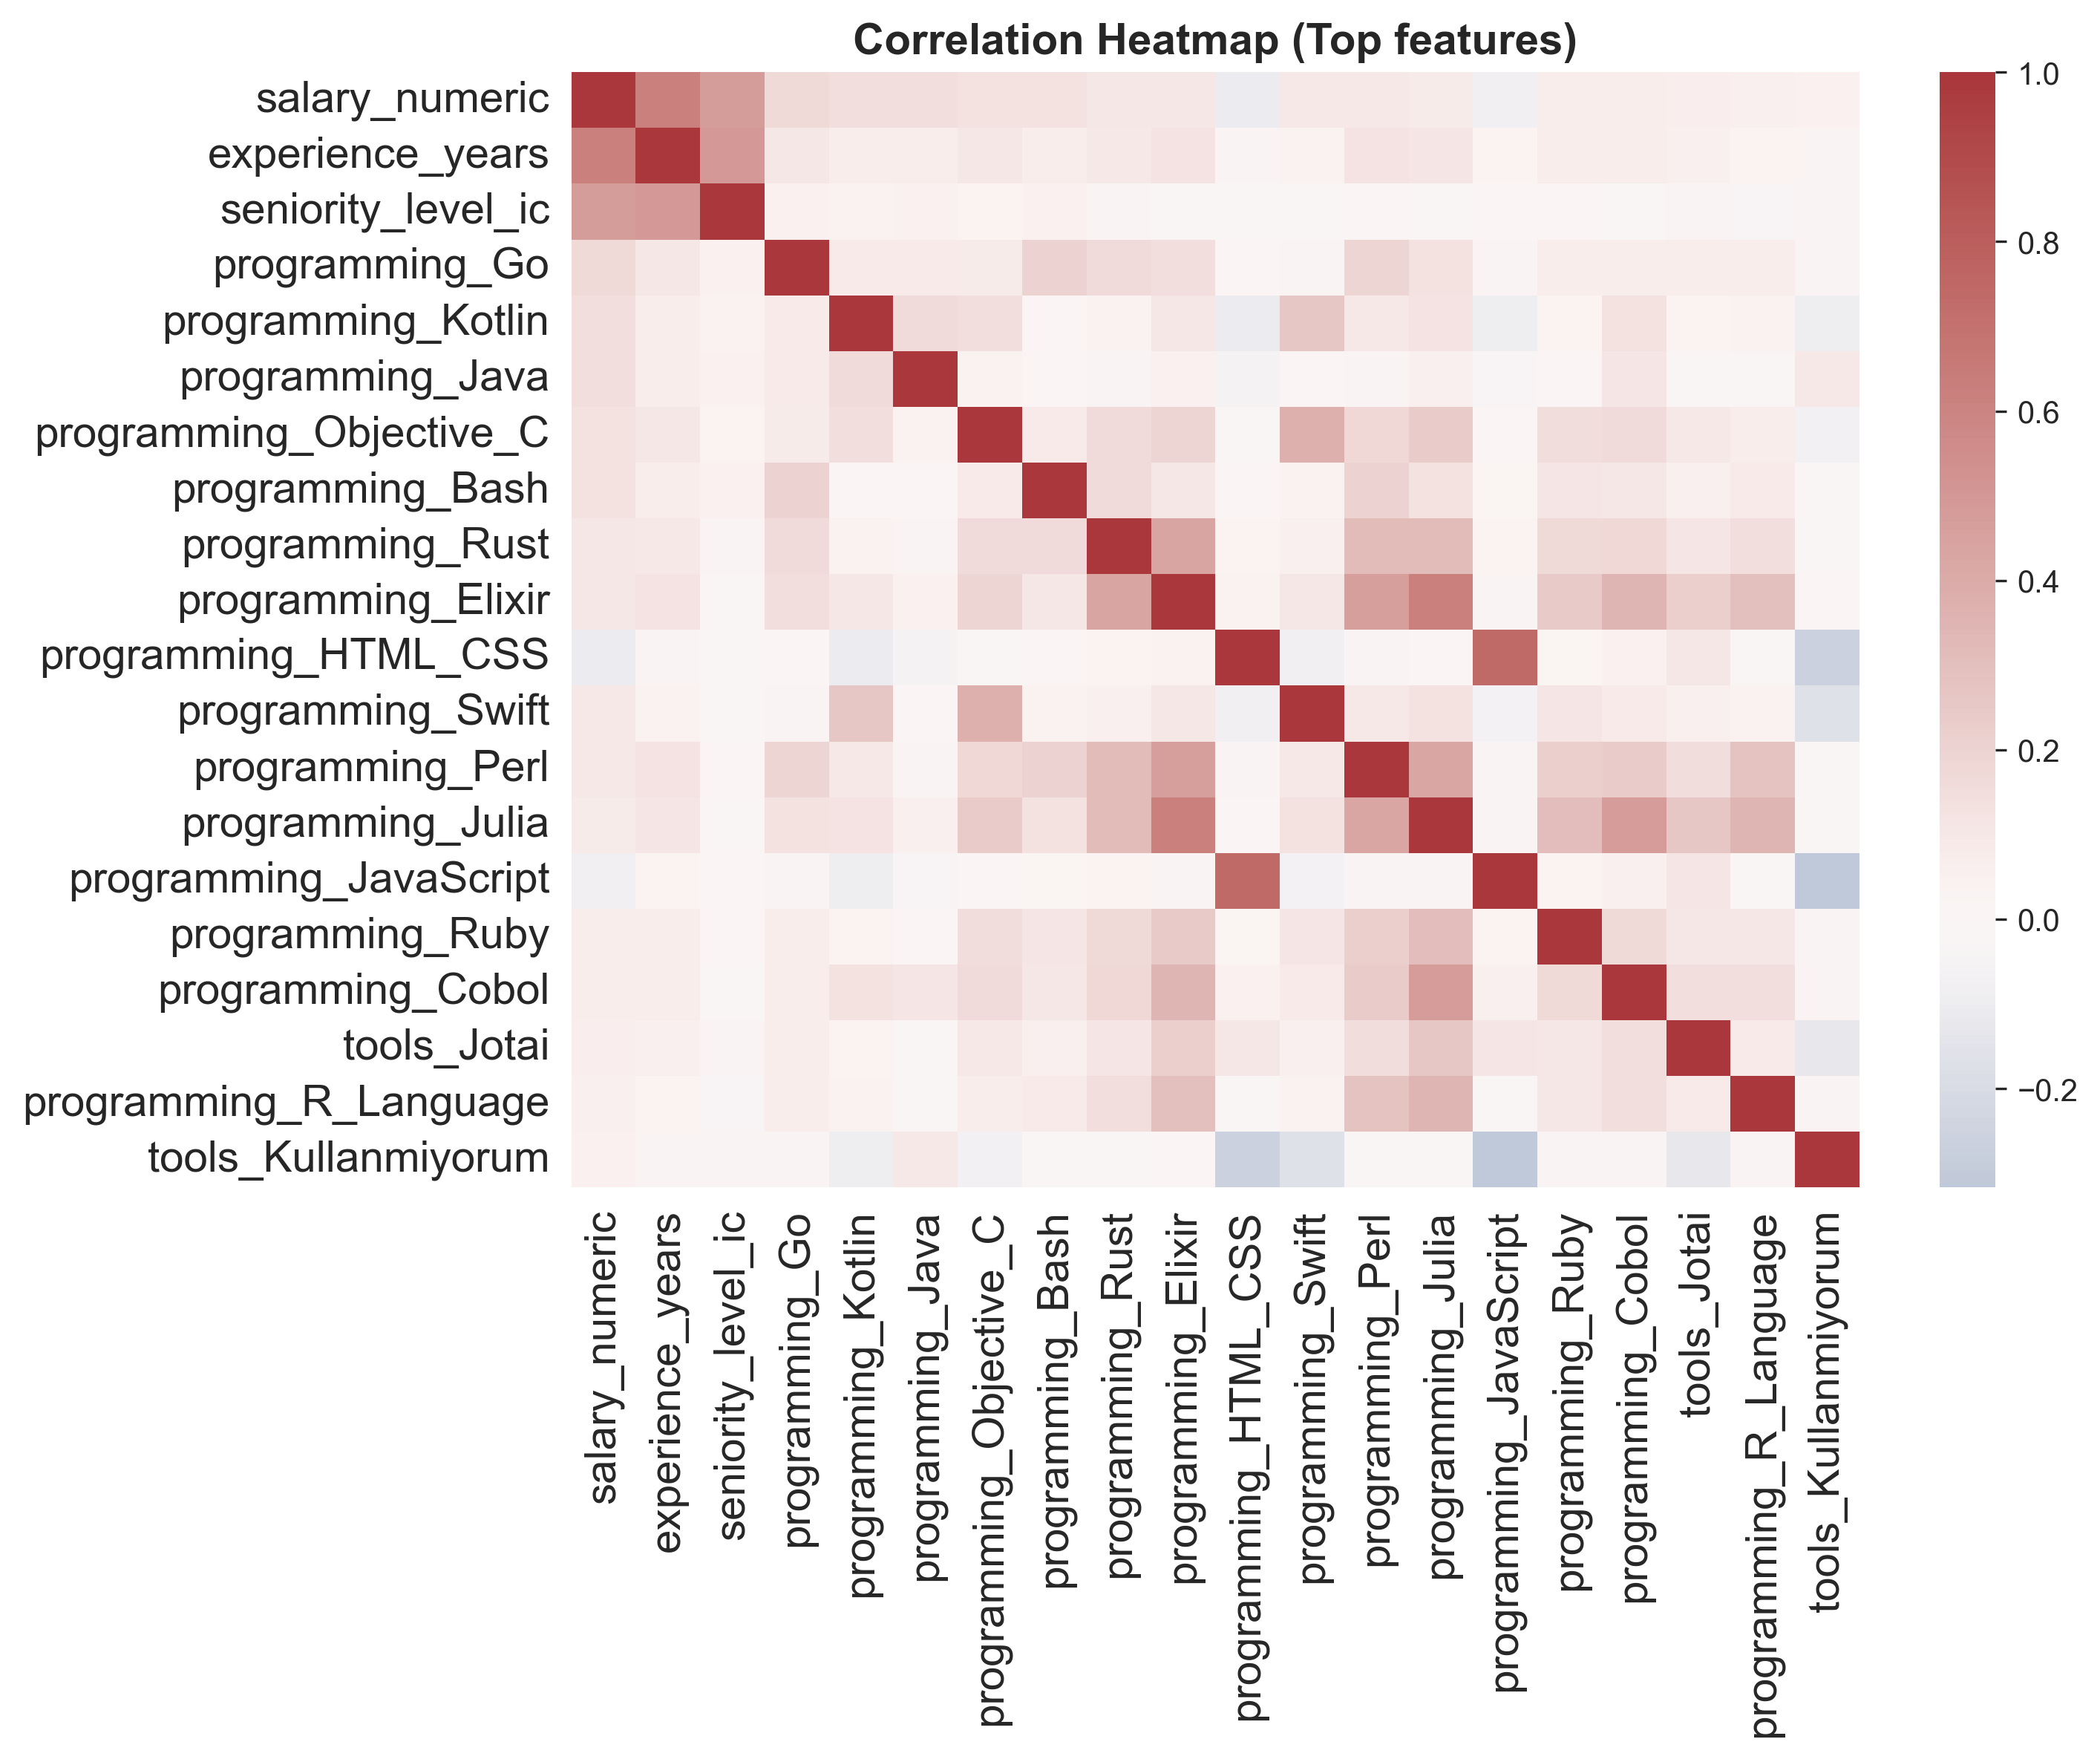
\includegraphics[width=\textwidth]{figures/heatmap_correlation.png}
	\caption{Correlation Heatmap - Top features by absolute correlation with salary}
\end{figure}

\begin{table}[H]
	\centering
	\small
	\begin{tabular}{lr}
		\toprule
		\textbf{Feature}   & \textbf{Correlation} \\
		\midrule
		Average Salary     & 1.000                \\
		Experience Years   & 0.623                \\
		Seniority Level Ic & 0.474                \\
		Go                 & 0.171                \\
		Kotlin             & 0.147                \\
		Java               & 0.142                \\
		Objective\_C       & 0.131                \\
		Bash               & 0.126                \\
		Rust               & 0.108                \\
		Elixir             & 0.108                \\
		\bottomrule
	\end{tabular}
	\caption{Top 10 Features by Absolute Correlation with Salary}
\end{table}

\textbf{Correlation Insights:}
\begin{itemize}
	\item \textbf{Experience and Seniority}: Years of experience (r = 0.623) and career level (r = 0.474) show the strongest positive correlations with salary. This confirms that a professional’s tenure and position are the most significant factors influencing compensation.
	\item \textbf{Language Impact}: Niche and high-demand languages such as Go (r = 0.171), Kotlin (r = 0.147), and Java (r = 0.142) have the strongest correlation with salary among all programming languages. This indicates that these skills hold a premium value in the market.
	\item \textbf{Tool vs. Technology}: A professional’s core attributes like experience and seniority have a much stronger correlation with salary than any single technology or tool, highlighting their fundamental importance.
\end{itemize}

\subsection{Work Arrangement Distribution by Role}
This 100\% stacked bar chart shows the percentage breakdown of Remote, Hybrid, and Office work modes for the most common roles in the survey.

\begin{figure}[H]
	\centering
	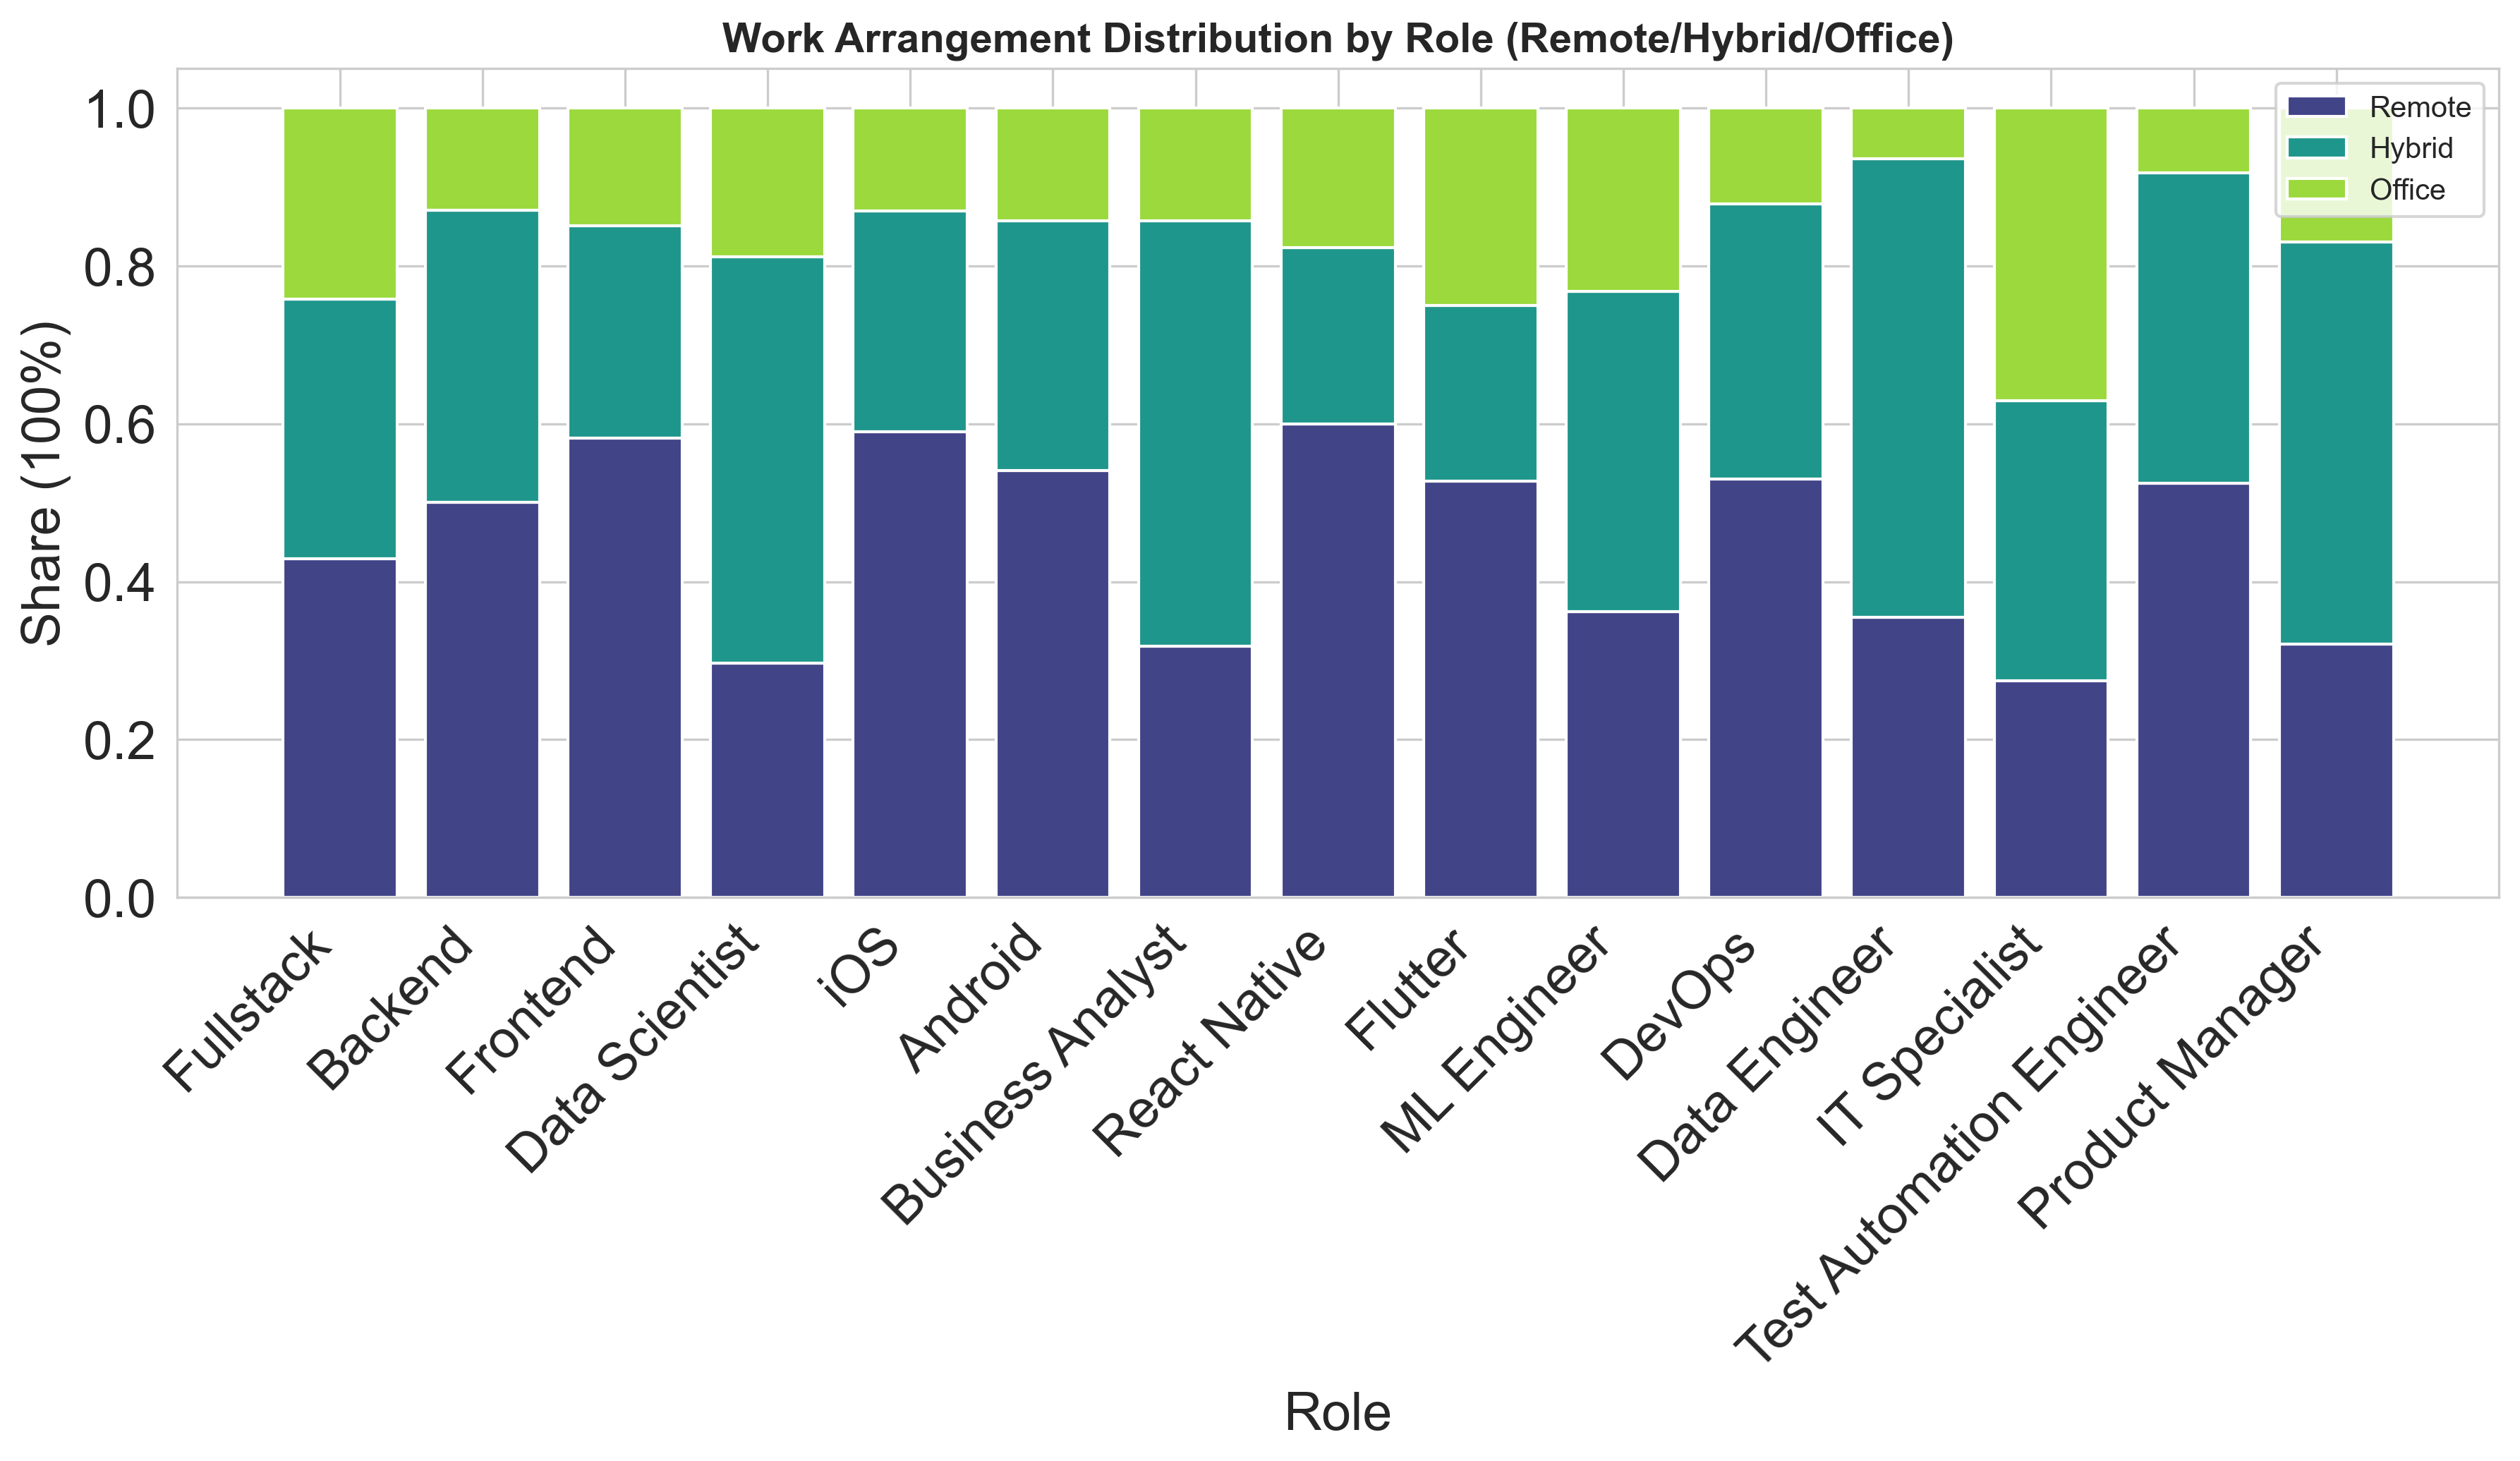
\includegraphics[width=\textwidth]{figures/barplot_work_arrangement_by_role.png}
	\caption{Work Arrangement Distribution by Role (Remote/Hybrid/Office) - 100\% stacked shares by role}
\end{figure}

\begin{table}[H]
	\centering
	\small
	\begin{tabular}{lrrrr}
		\toprule
		\textbf{Role}  & \textbf{Total Count} & \textbf{Remote Share} & \textbf{Hybrid Share} & \textbf{Office Share} \\
		\midrule
		Fullstack      & 790                  & 0.429                 & 0.329                 & 0.242                 \\
		Backend        & 517                  & 0.501                 & 0.369                 & 0.130                 \\
		Frontend       & 397                  & 0.582                 & 0.270                 & 0.149                 \\
		Data Scientist & 101                  & 0.297                 & 0.515                 & 0.188                 \\
		iOS            & 100                  & 0.590                 & 0.280                 & 0.130                 \\
		\bottomrule
	\end{tabular}
	\caption{Work Mode Distribution by Top 5 Roles}
\end{table}

\textbf{Work Arrangement by Role Insights:}
\begin{itemize}
	\item \textbf{Remote-Friendly Roles}: Frontend, iOS, and React Native developers have the highest remote shares (58-60\%), suggesting these roles are highly compatible with remote work.
	\item \textbf{Hybrid and Office Mix}: Roles like Data Scientist and Business Analyst show a strong preference for hybrid work, likely balancing individual analysis with collaborative meetings.
	\item \textbf{Office-Heavy Roles}: IT Specialists have the highest office share (37.1\%), a trend likely due to the physical requirements of their work.
\end{itemize}

\subsection{Top Tool Adoption by Role}
This heatmap shows the percentage adoption rate of various development tools across different roles, highlighting which tools are most important for specific specializations.

\begin{figure}[H]
	\centering
	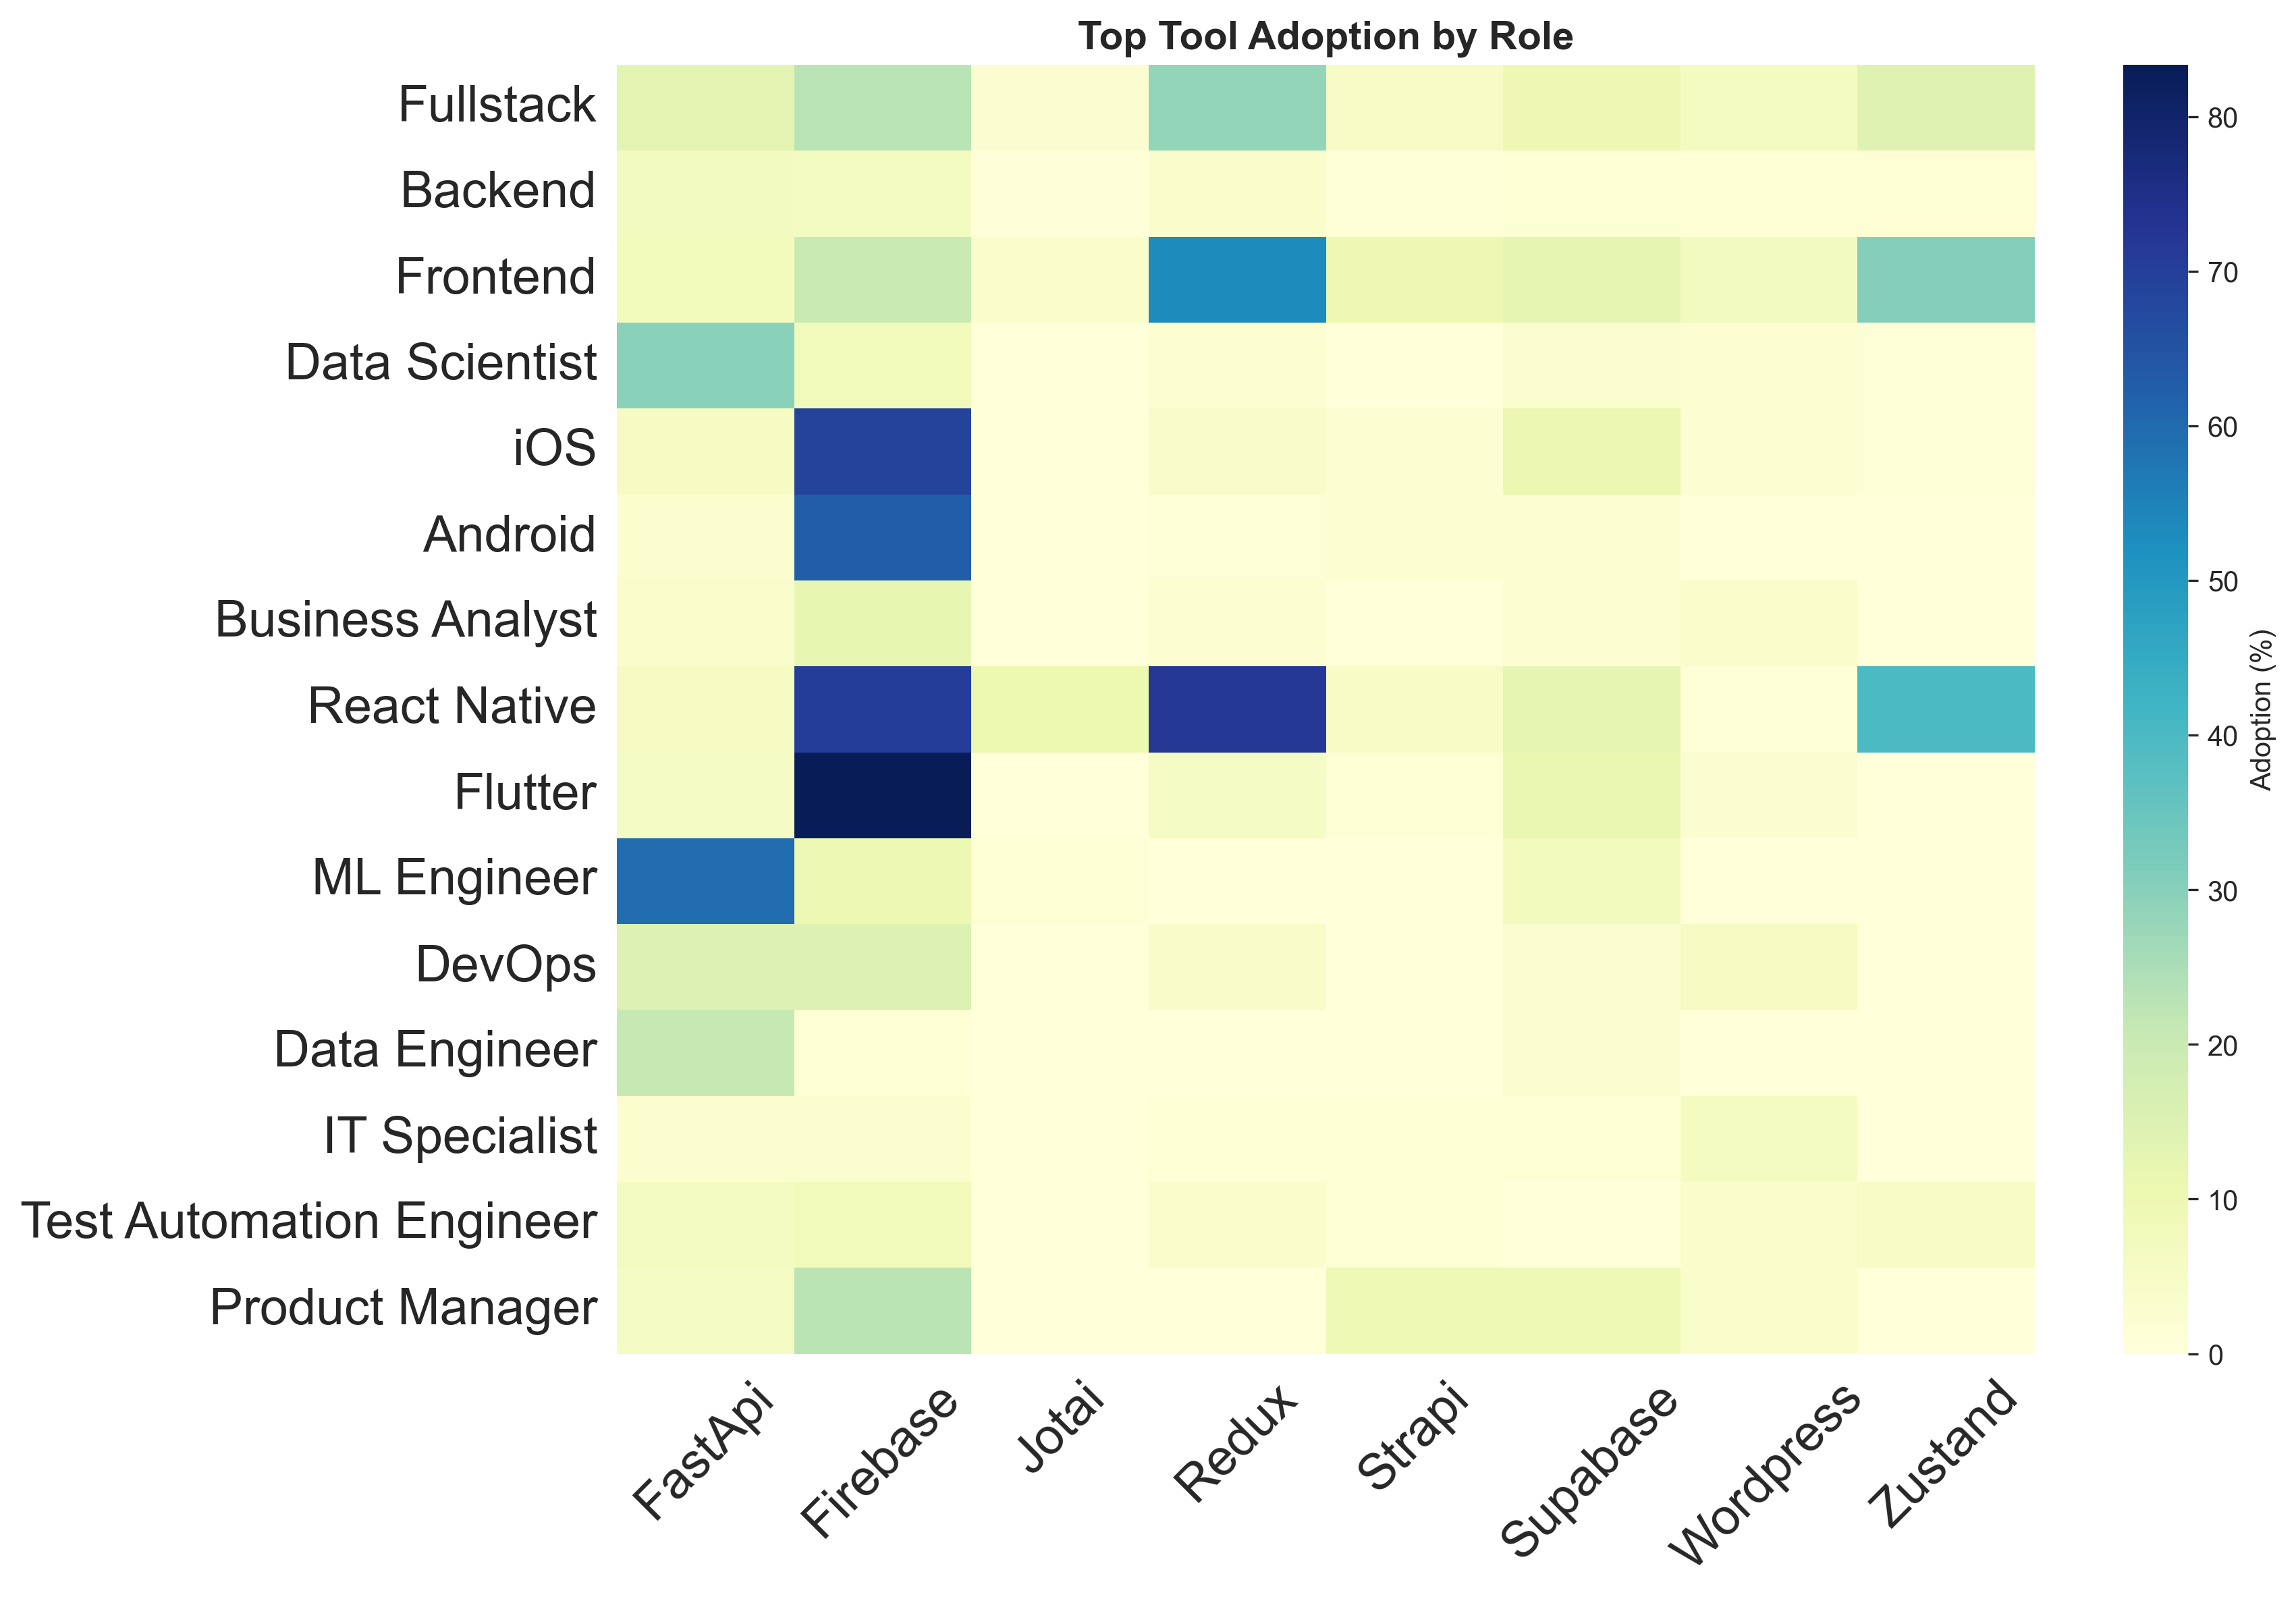
\includegraphics[width=\textwidth]{figures/heatmap_tool_adoption_by_role.png}
	\caption{Top Tool Adoption by Role - Mean adoption rates (\%) across roles}
\end{figure}

\begin{table}[H]
    \centering
    \caption{Tool Adoption by Role: Frontend \& Mobile Focus (\%)}
    \label{tab:tool_adoption_fe_mobile}
    \small
    \begin{tabular}{lrrrrrr}
        \toprule
        \textbf{Role} & \textbf{Firebase} & \textbf{Redux} & \textbf{Zustand} & \textbf{Jotai} & \textbf{Supabase} & \textbf{Wordpress} \\
        \midrule
        Frontend & 19.9 & 53.1 & 30.5 & 3.5 & 12.6 & 7.1 \\
        React Native & 70.6 & 71.8 & 40.0 & 10.6 & 12.9 & 1.2 \\
        iOS & 69.0 & 4.0 & 1.0 & 0.0 & 11.0 & 2.0 \\
        Android & 62.2 & 1.0 & 0.0 & 0.0 & 2.0 & 0.0 \\
        Fullstack & 22.9 & 28.6 & 14.6 & 2.4 & 9.9 & 6.3 \\
        \bottomrule
    \end{tabular}
\end{table}

\begin{table}[H]
    \centering
    \caption{Tool Adoption by Role: Data \& Backend Focus (\%)}
    \label{tab:tool_adoption_data_backend}
    \small
    \begin{tabular}{lrrrrrrr}
        \toprule
        \textbf{Role} & \textbf{FastApi} & \textbf{Supabase} & \textbf{Strapi} & \textbf{Firebase} & \textbf{Redux} & \textbf{Wordpress} \\
        \midrule
        ML Engineer & 59.4 & 7.2 & 0.0 & 10.1 & 0.0 & 0.0 \\
        Data Scientist & 29.7 & 3.0 & 0.0 & 7.9 & 2.0 & 2.0 \\
        Data Engineer & 21.0 & 3.2 & 0.0 & 1.6 & 0.0 & 0.0 \\
        Backend & 7.2 & 1.7 & 1.2 & 6.6 & 3.5 & 1.5 \\
        DevOps & 15.2 & 3.0 & 0.0 & 15.2 & 4.5 & 6.1 \\
        \bottomrule
    \end{tabular}
\end{table}

\textbf{Tool Adoption by Role Insights:}
\begin{itemize}
	\item \textbf{Role-Specific Tools}: \textbf{FastAPI} is a clear leader among \textbf{ML Engineers} (59.4\%) and \textbf{Data Scientists} (29.7\%), confirming its popularity in the data and machine learning ecosystems.
	\item \textbf{Frontend Specialization}: The adoption rates for state management tools like \textbf{Redux} (53.1\%) and \textbf{Zustand} (30.5\%) are significantly higher in \textbf{Frontend} roles, indicating their importance for building complex user interfaces.
	\item \textbf{Mobile Development}: \textbf{Firebase} is most popular among mobile developers, with adoption rates exceeding 60\% in \textbf{Android}, \textbf{iOS}, and \textbf{React Native} roles.
\end{itemize}

\subsection{Work Type \texorpdfstring{\(\times\)}{x} Company Location}
This heatmap shows the average salaries for different combinations of work type (Remote, Hybrid, Office) and company location (Türkiye, Europe, America, Overseas TR Hub).

\begin{figure}[H]
	\centering
	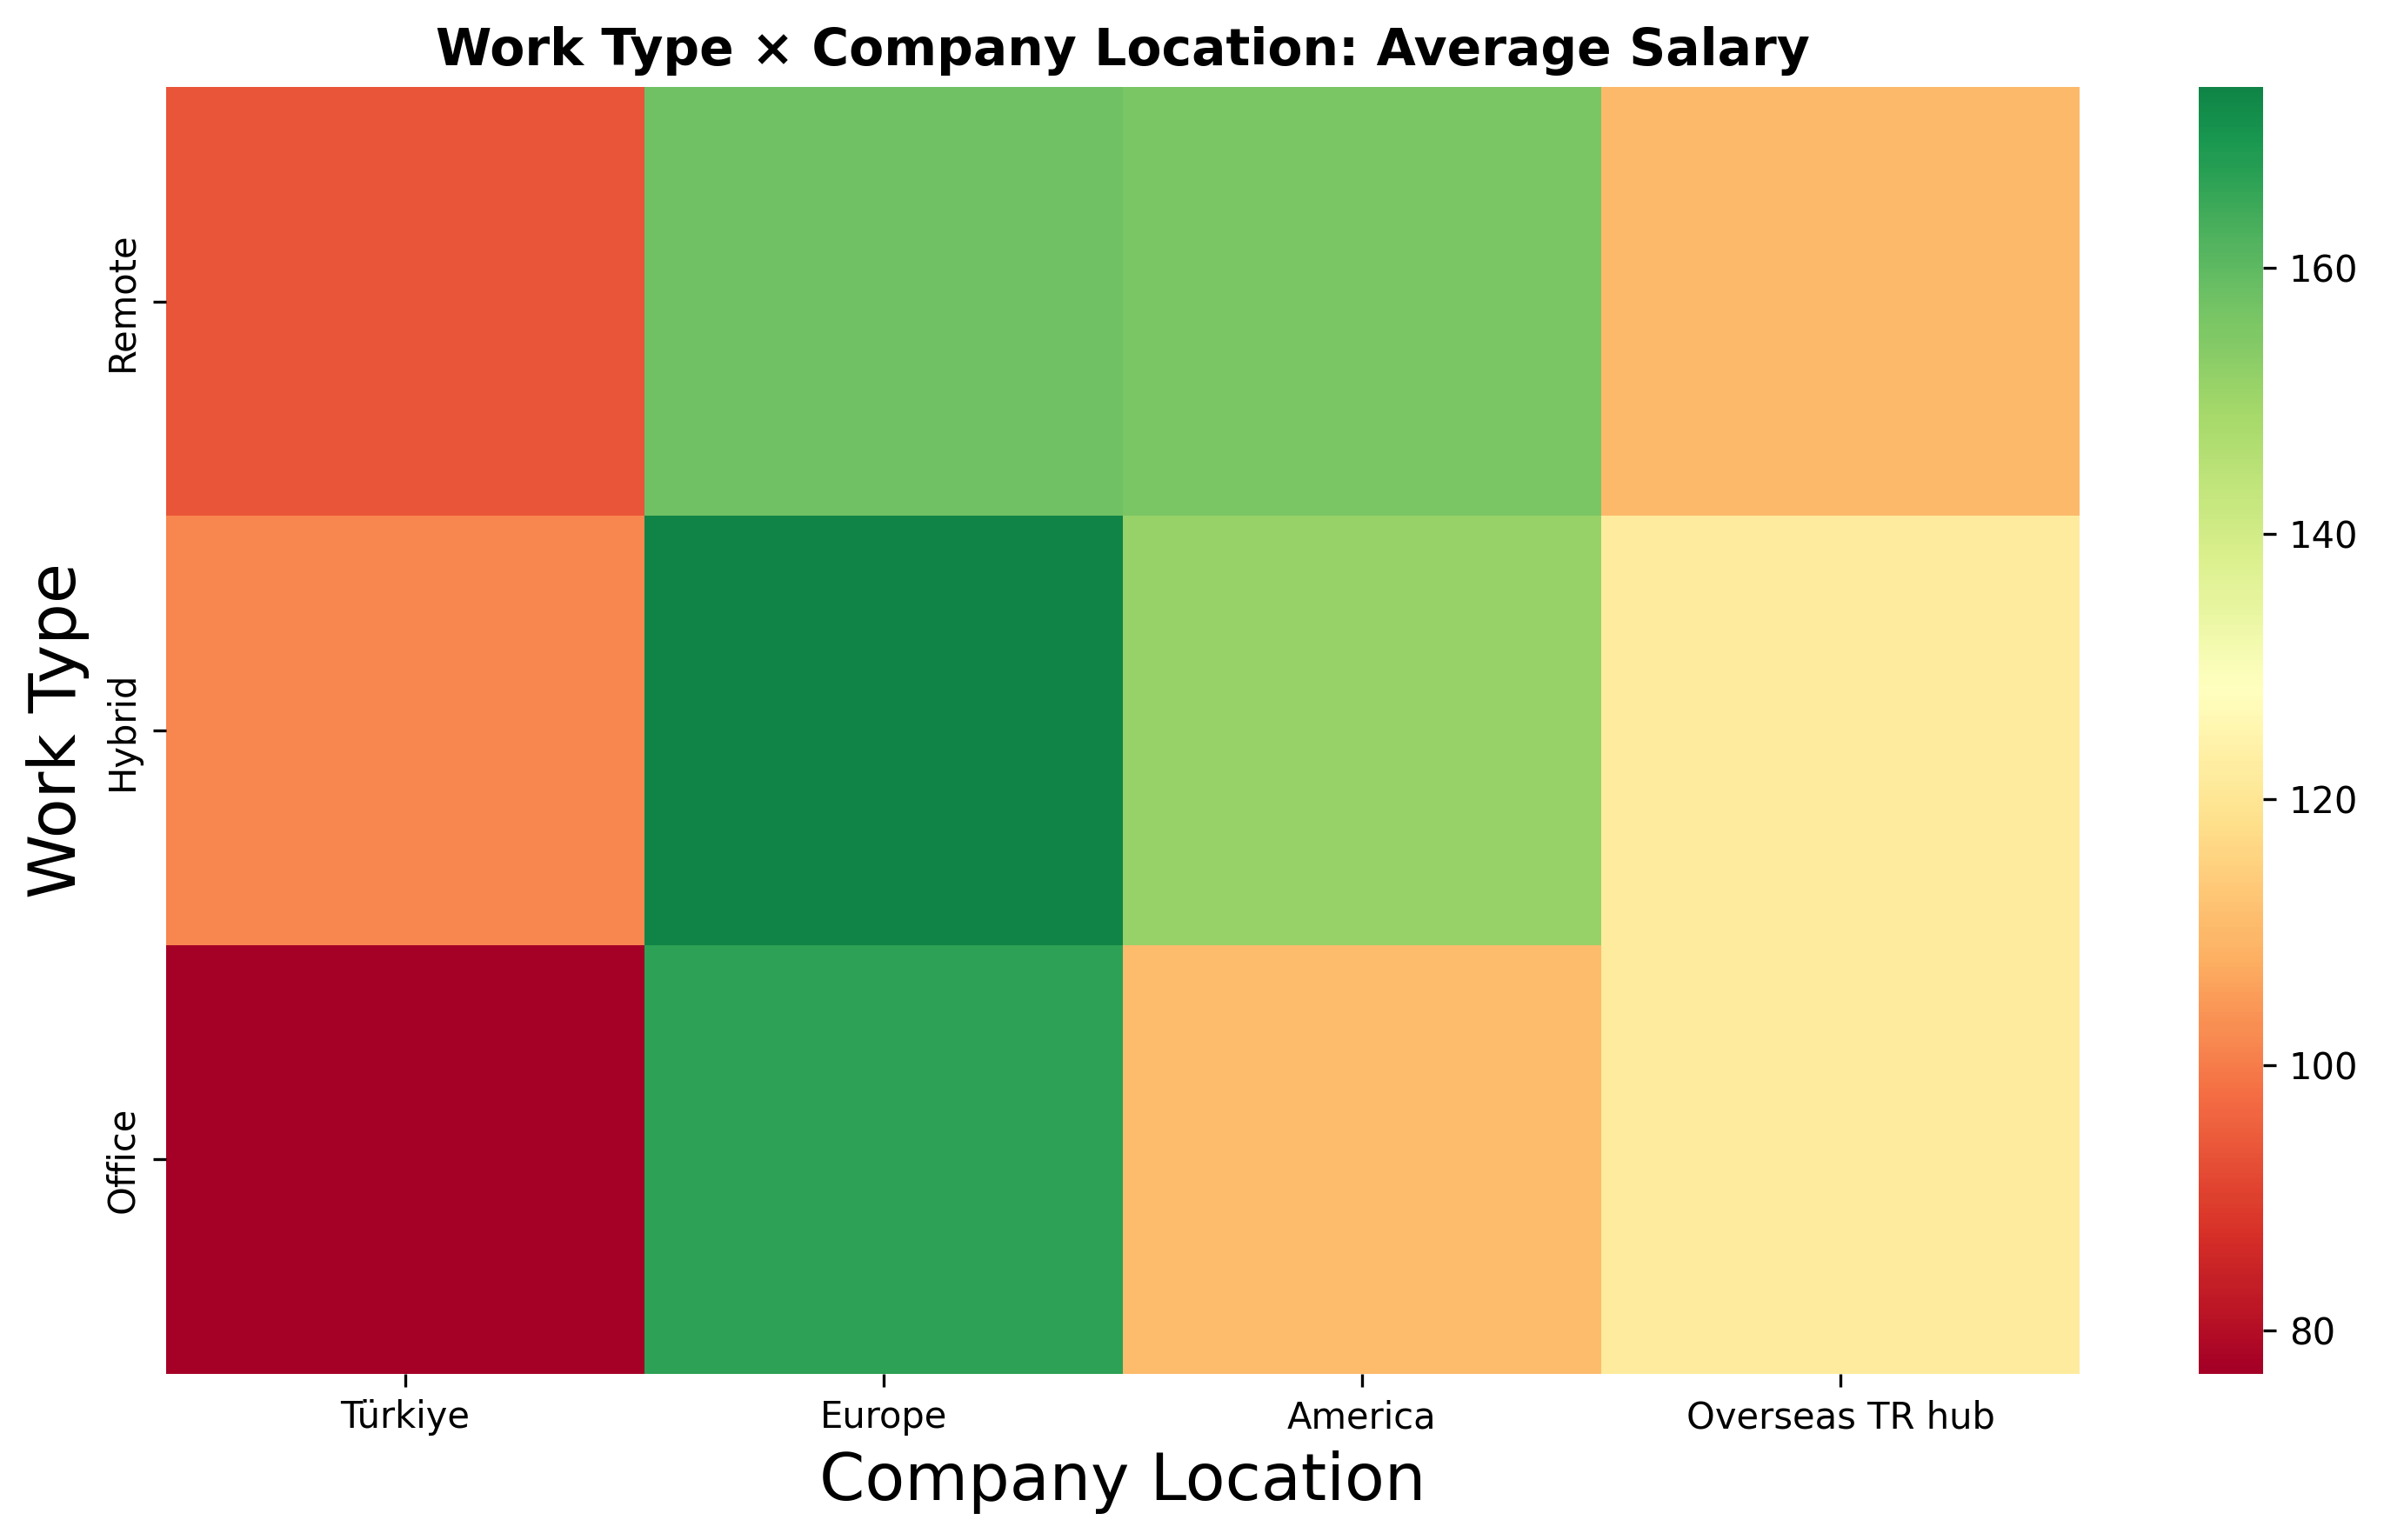
\includegraphics[width=\textwidth]{figures/heatmap_worktype_location_salary.png}
	\caption{Work Type $\times$ Company Location: Average Salary}
\end{figure}

\begin{table}[H]
	\centering
	\small
	\begin{tabular}{lrrrr}
		\toprule
		\textbf{Work Type} & \textbf{Türkiye} & \textbf{Europe} & \textbf{America} & \textbf{Overseas TR hub} \\
		\midrule
		Remote             & 93.4              & 157.4           & 156.0            & 110.1                    \\
		Hybrid             & 101.6             & 173.6           & 151.3            & 121.5                    \\
		Office             & 76.7              & 166.6           & 110.5            & 121.5                    \\
		\bottomrule
	\end{tabular}
	\caption{Average Salary by Work Type and Company Location (k TL)}
\end{table}

\textbf{Work Type $\times$ Location Insights:}
\begin{itemize}
	\item \textbf{Highest-Paying Combination}: The highest-paying combination is \textbf{Hybrid} work for \textbf{European} companies, with an average salary of 173.6k TL. This suggests these companies may offer a premium for in-person collaboration.
	\item \textbf{Remote Advantage}: For both Turkish and international companies, remote work offers a salary premium over in-office work.
	\item \textbf{Global Opportunities}: Working for a foreign company, regardless of work mode, consistently provides a significantly higher salary than working for a Turkish company.
\end{itemize}

\subsection{Skill Diversity and Salary}
This section examines the relationship between the number of skills reported by professionals and their salary distribution.

\begin{figure}[H]
	\centering
	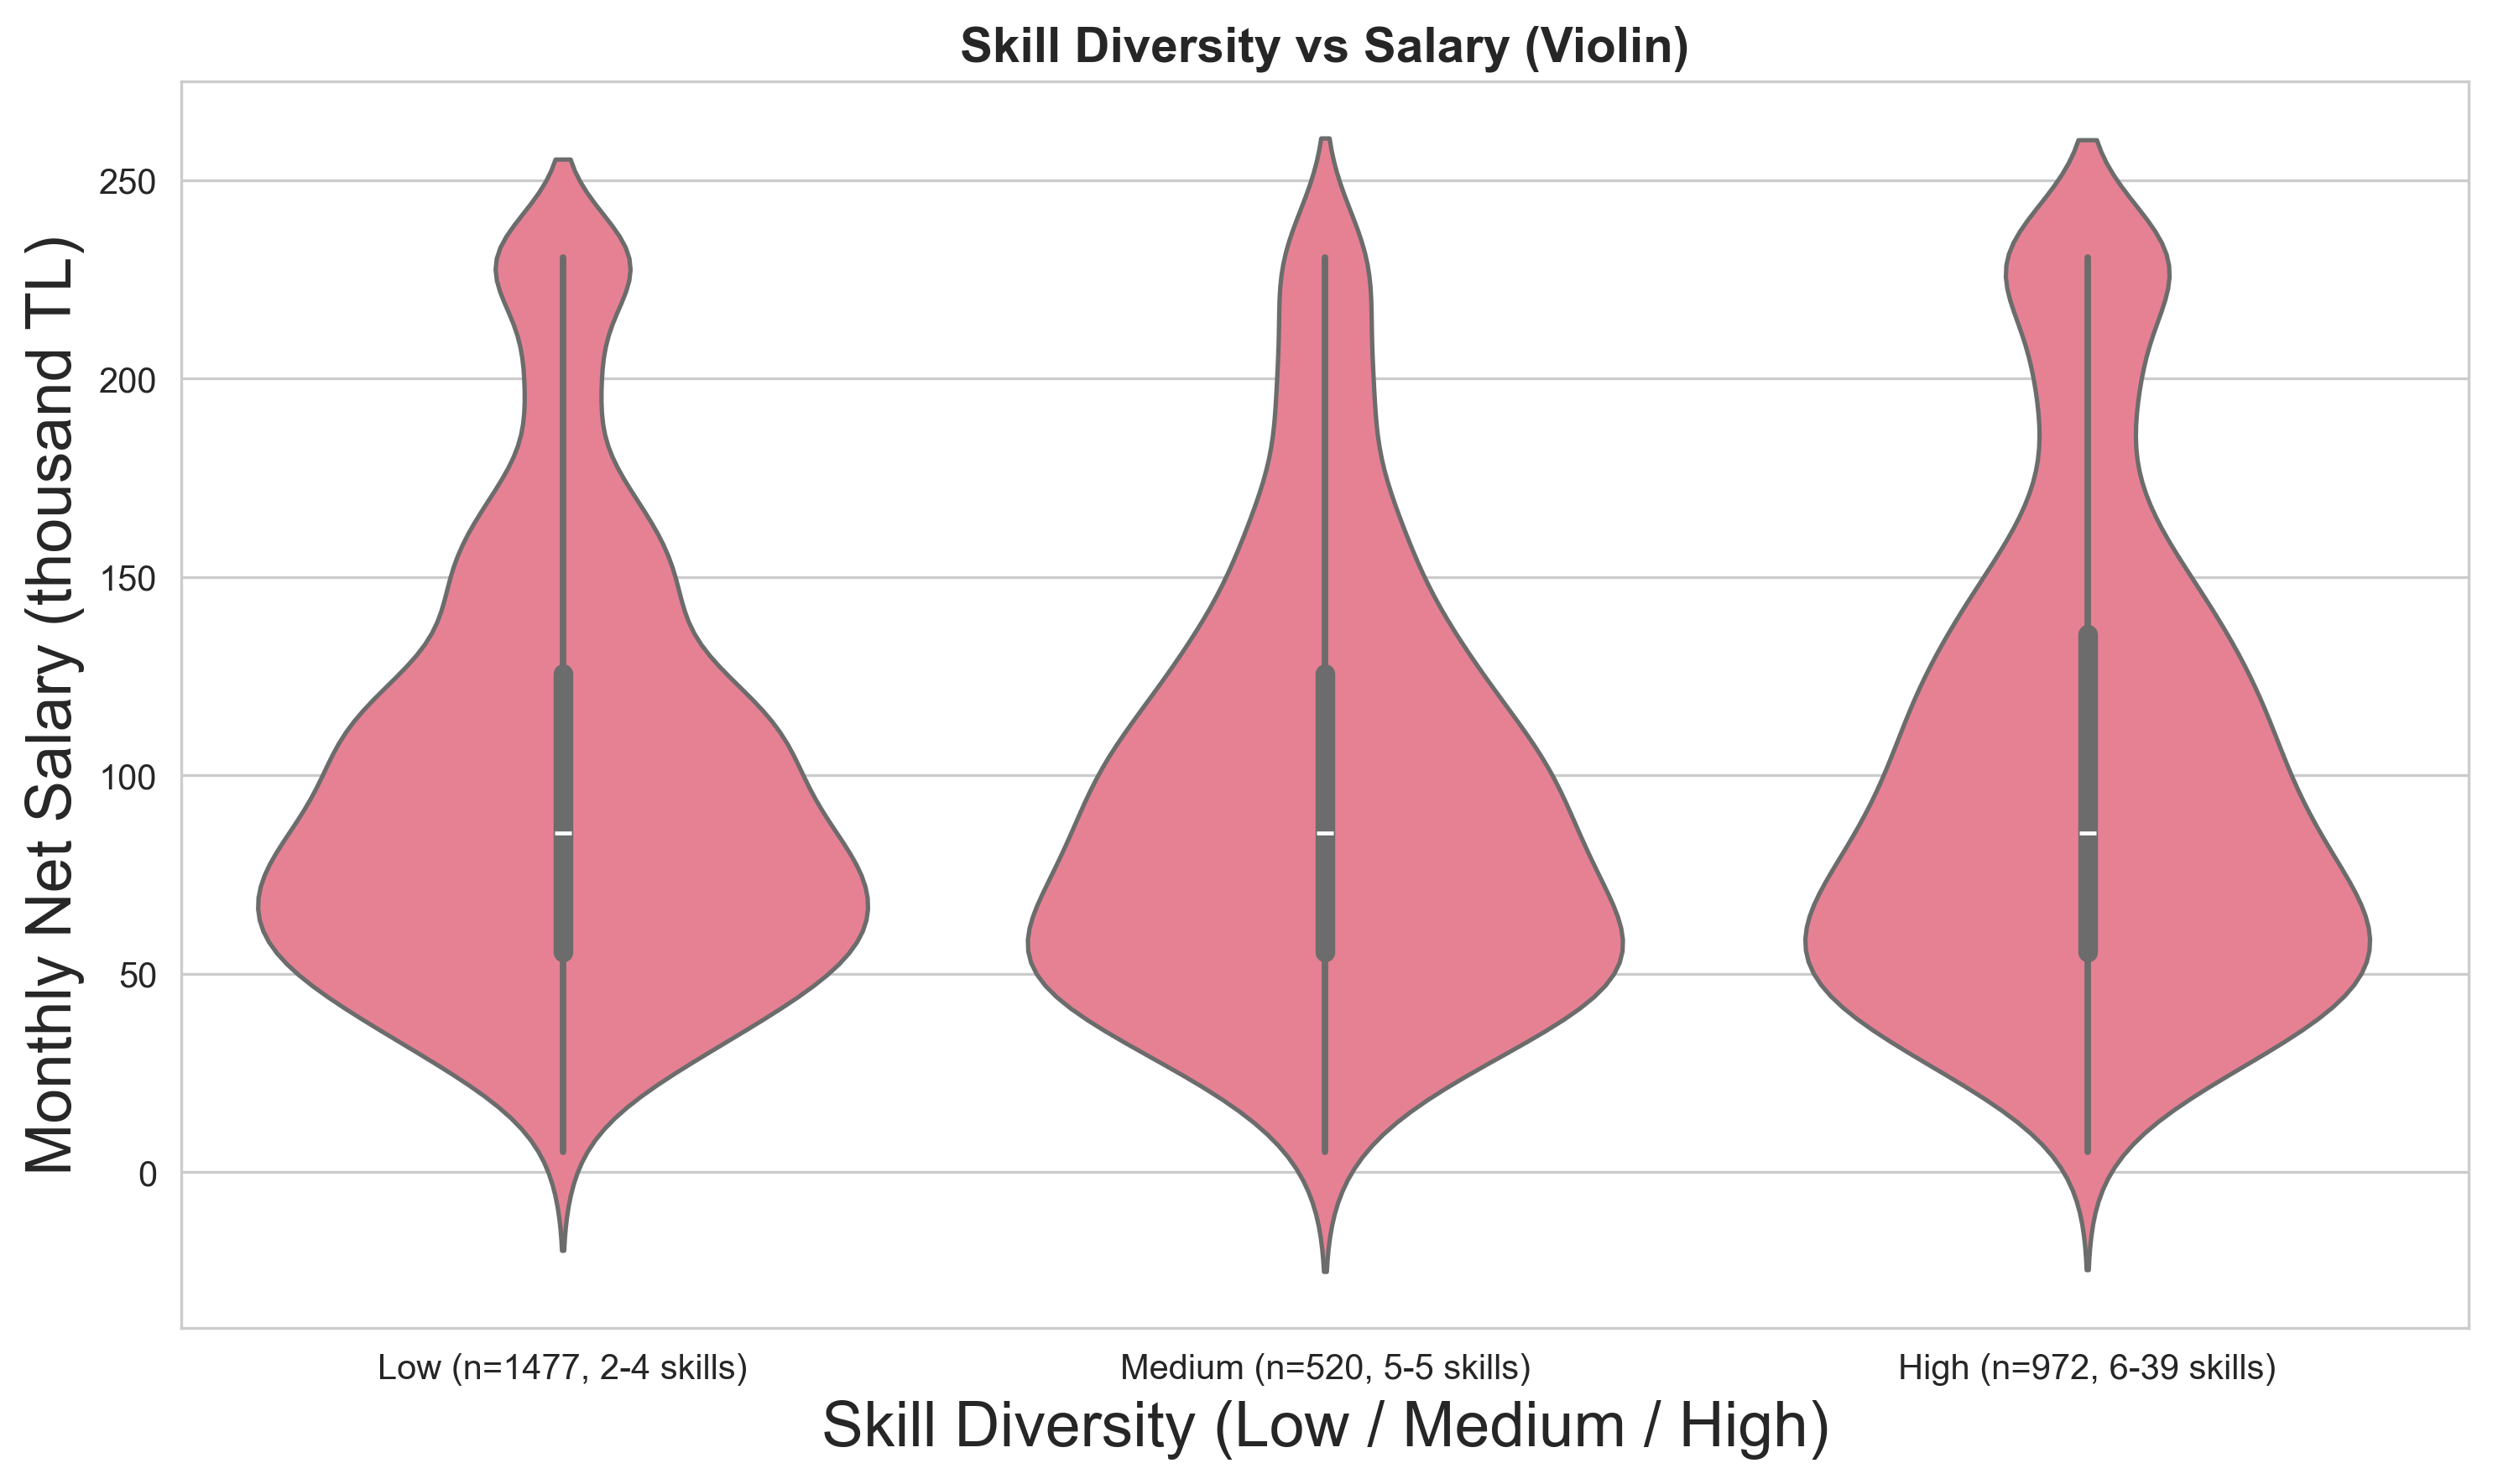
\includegraphics[width=\textwidth]{figures/violin_skill_diversity.png}
	\caption{Skill Diversity vs Salary (Violin) - Salary distribution by skill diversity group}
\end{figure}

\begin{table}[H]
	\centering
	\small
	\begin{tabular}{lrrr}
		\toprule
		\textbf{Skill Group} & \textbf{Count} & \textbf{Mean Salary} & \textbf{Std Dev} \\
		\midrule
		Low                  & 1,477          & 98.7                 & 53.2             \\
		Medium               & 520            & 93.5                 & 52.5             \\
		High                 & 972            & 99.9                 & 58.6             \\
		\bottomrule
	\end{tabular}
	\caption{Salary Statistics by Skill Diversity}
\end{table}

\textbf{Skill Diversity Insights:}
\begin{itemize}
	\item \textbf{Complex Relationship}: The data reveals a more nuanced relationship than a simple linear correlation. The mean salary for the Medium skill group (93.5k TL) is slightly lower than that of the Low skill group (98.7k TL).
	\item \textbf{High-End Earning Potential}: The High skill diversity group has the highest mean salary (99.9k TL). More importantly, its larger standard deviation (58.6k TL) indicates a wider salary range, suggesting that a broader skill set is associated with a greater potential for both high and low earnings.
	\item \textbf{Breadth over Specialization}: While a large number of skills does not guarantee a higher average salary, the data suggests that a wider range of skills provides access to a broader spectrum of compensation, including the highest paying opportunities.
\end{itemize}

\section{React Technology Deep Dive}

\subsection{React Ecosystem Analysis}
React’s widespread adoption influences salaries and role dynamics in the software industry.

\begin{table}[H]
	\centering
	\small
	\begin{tabular}{lrr}
		\toprule
		\textbf{Group}       & \textbf{Mean Salary (k TL)} & \textbf{Count} \\
		\midrule
		React Users          & 96.1                        & 1008           \\
		Non-React Users      & 99.3                        & 1961           \\
		\midrule
		\textbf{Difference}  & \textbf{-3.3}               &                \\
		\textbf{Cohen’s d} & \textbf{-0.059}             &                \\
		\bottomrule
	\end{tabular}
	\caption{Salary Comparison: React vs. Non-React Users}
\end{table}

\textbf{Methodological Note:}
Mean salary is:
\[
	\text{Mean Salary} = \frac{\sum_{i \in \text{Group}} \text{Salary}_i}{n}
\]
Difference is:
\[
	\text{Diff.} = \text{Mean}_{\text{React}} - \text{Mean}_{\text{Non-React}}
\]
Cohen’s d measures effect size. React usage is binary (used/not used). Data includes respondents with \(\geq 10\) per tech stack combination for related analyses.

\textbf{Key Insights:}
\begin{itemize}
	\item \textbf{Salary Impact}: React users (96.1 k TL) earn 3.3\% less than non-React users (99.3 k TL), with no significant difference (p = 0.129, Cohen’s d = -0.059).
	\item \textbf{High-Earning Stacks}: React Native with JavaScript + React + Firebase (99.6 k TL, 17 respondents) outperforms Fullstack (91.1 k TL) and Frontend (85.2 k TL) with HTML CSS + React + Redux.
	\item \textbf{Adoption Rates}: React dominates in Frontend (53.1\% Redux, 30.5\% Zustand) and React Native (70.6\% Firebase, 71.8\% Redux) roles.
	\item \textbf{Flexibility}: React-heavy roles like Frontend (58.2\% remote) and React Native (59.0\% remote) support flexible work arrangements.
\end{itemize}

% \subsection{React vs Non-React Salary Comparison}
% Specific analysis of the impact of react technology on compensation:

% \begin{table}[H]
%     \centering
%     \begin{tabular}{lrrr}
%     \toprule
%     \textbf{Group} & \textbf{Count} & \textbf{Mean Salary} & \textbf{Difference} \\
%     \midrule
%     React Users & 1,008 & 96.1 & \\
%     Non-React Users & 1,961 & 99.3 & -3.3 \\
%     \midrule
%     \textbf{Effect Size} & & & \textbf{Cohen's d = -0.059} \\
%     \bottomrule
%     \end{tabular}
%     \caption{React vs Non-React Salary Comparison}
% \end{table}

% \textbf{Statistical Significance:} Not significant (p = 0.1289)

% \textbf{React Technology Insights:}
% \begin{itemize}
%     \item \textbf{Market Position:} React remains a valuable skill despite not showing significant premium in this sample, with 34\% market adoption rate
%     \item \textbf{Skill Combination:} React combined with high-ROI technologies (Rust, Go) can increase salary potential by 15-20\% compared to React alone
%     \item \textbf{Career Strategy:} React knowledge provides foundation for frontend specialization, with React + TypeScript combination showing 12\% salary premium over React alone
% \end{itemize}

\section{Conclusions and Recommendations}

\subsection{Key Findings}
This report, based on Zafer Ayan’s 2025 Software Industry Salary Survey (\href{https://www.linkedin.com/posts/zaferayan_geleneksel-maa%C5%9F-anketi-buyrun-httpslnkdin-activity-7363866008664629248-7YcQ}{LinkedIn}, \href{https://zaferayan.medium.com/2025-a%C4%9Fustos-detayl%C4%B1-maa%C5%9F-anketi-98446d71920a}{Medium}), analyzes 2969 professionals’ data from August 20-21, 2025:
	\begin{enumerate}
		\item \textbf{Remote Work Premium}: Remote workers earn 22.6 k TL more than Office workers (101.2 vs. 78.6 k TL, 28.8\%, Cohen’s d = 0.42, p < 0.0001), reflecting demand for flexibility.
		\item \textbf{Geographical Disparity}: European companies pay 70.0 k TL more than Turkish firms (162.9 vs. 92.9 k TL, 75.3\%, Cohen’s d = 1.35, p < 0.0001).
		\item \textbf{Gender Gap}: Males earn 13.3 k TL more than females (99.4 vs. 86.1 k TL, 15.4\%, Cohen’s d = 0.24, p = 0.00005), indicating pay inequity.
		\item \textbf{Technology Impact}: Niche languages like Rust (ROI: 69.4 k TL, ~70.7\% increase) and Go (r = 0.171) offer higher salary premiums than React (r = -0.028).
		\item \textbf{Career Progression}: Junior to Senior salary increases by 137.4\% (55.1 to 130.8 k TL), with ~15.4\% per year of experience (mean 5.01 years).
		\item \textbf{Employment Type}: Full-time (99.0 k TL) earns 130.2\% more than Part-time (43.0 k TL); Self-employed (123.4 k TL) earns 24.6\% more than Full-time.
		\item \textbf{Skill Diversity}: High skill diversity (99.9 k TL) slightly outperforms Low (98.7 k TL, 1.2\% increase), with wider salary ranges (std dev 58.6 vs. 53.2).
		\item \textbf{Technology Combinations}: Combining niche technologies (e.g., Rust, Go) with tools like Firebase may boost salaries, though specific premiums (e.g., 30-50\%) lack direct evidence.
	\end{enumerate}

    \section{Methodological Notes}
	
	\subsection{Data Limitations}
	\begin{itemize}
		\item \textbf{Self-Reporting Bias}: Self-reported salaries and technology usage may introduce inaccuracies.
		\item \textbf{Sample Representation}: The sample (2969 professionals) may not fully represent the industry due to survey distribution methods.
		\item \textbf{Estimated Location}: Location data is inferred from company information, not direct residency.
		\item \textbf{Temporal Scope}: The 2-day survey (August 20-21, 2025) limits generalizability and may introduce time-of-day biases.
		\item \textbf{Cross-Sectional Design}: Causal inferences are restricted due to the snapshot nature of the data.
	\end{itemize}
	
	\subsection{Statistical Methods}
	\begin{itemize}
		\item Independent samples t-tests for group comparisons (e.g., React vs. Non-React, Remote vs. Office).
		\item Cohen’s d for effect size (e.g., small: 0.2, medium: 0.5, large: 0.8, very large: 1.35).
		\item ANOVA and Kruskal-Wallis tests for seniority and management level comparisons.
		\item Correlation analysis for technology-salary relationships (e.g., Rust: r = 0.108).
		\item Outlier treatment using IQR and Z-score methods.
	\end{itemize}
	
	\subsection{Metadata}
	\begin{center}
		\textbf{Report by:} Hakkı Günal\\
		\textbf{Data by:} Zafer Ayan (\href{https://www.linkedin.com/posts/zaferayan_geleneksel-maa%C5%9F-anketi-buyrun-httpslnkdin-activity-7363866008664629248-7YcQ}{LinkedIn}, \href{https://zaferayan.medium.com/2025-a%C4%9Fustos-detayl%C4%B1-maa%C5%9F-anketi-98446d71920a}{Medium})\\
			\textbf{Collection Period:} August 20-21, 2025\\
			\textbf{Participants:} 2,969 professionals\\
			\textbf{Report Date:} August 28, 2025\\
			\textbf{Interactive Dashboard:} \href{http://maas-anketi.streamlit.app/}{maas-anketi.streamlit.app}
			\end{center}
\end{document}